% !TEX encoding = UTF-8 Unicode
\documentclass[12pt,twoside,a4paper]{report}
\setcounter{tocdepth}{2}
\usepackage[]{geometry}
\setlength{\headheight}{15.0pt}
\usepackage[utf8]{inputenc}
\usepackage[T1]{fontenc}
\usepackage[francais]{babel}
\usepackage{graphicx}

% header
\usepackage{fancyhdr}
\pagestyle{fancy}

% code listings
\usepackage{listings}

\usepackage[usenames,dvipsnames,svgnames,table,xcdraw]{xcolor}
\usepackage{pdfpages}

\definecolor{olivegreen}{HTML}{3C8031}

\usepackage[T1]{fontenc}
\usepackage[scaled]{beramono}
\newcommand\Small{\fontsize{9}{9.2}\selectfont}
\newcommand*\LSTfont{\Small\ttfamily\SetTracking{encoding=*}{-60}\lsstyle}

\definecolor{lightgray}{rgb}{.9,.9,.9}
\definecolor{darkgray}{rgb}{.4,.4,.4}
\definecolor{purple}{rgb}{0.65, 0.12, 0.82}
\lstdefinelanguage{JavaScript}{
  keywords={break, case, catch, continue, debugger, default, delete, do, else, false, finally, for, function, if, in, instanceof, new, null, return, switch, this, throw, true, try, typeof, var, void, while, with},
  morecomment=[l]{//},
  morecomment=[s]{/*}{*/},
  morestring=[b]',
  morestring=[b]",
  ndkeywords={class, export, boolean, throw, implements, import, this},
  keywordstyle=\color{blue}\bfseries,
  ndkeywordstyle=\color{darkgray}\bfseries,
  identifierstyle=\color{black},
  commentstyle=\color{purple}\ttfamily,
  stringstyle=\color{red}\ttfamily,
  sensitive=true
}

\lstset{ %
  basicstyle=\footnotesize\ttfamily,        % the size of the fonts that are used for the code
  breakatwhitespace=false,         % sets if automatic breaks should only happen at whitespace
  breaklines=true,                 % sets automatic line breaking
  commentstyle=\color{olivegreen},    % comment style
  escapeinside={\%*}{*)},          % if you want to add LaTeX within your code
  extendedchars=true,              % lets you use non-ASCII characters; for 8-bits encodings only, does not work with UTF-8
  frame=single,	                   % adds a frame around the code
  keepspaces=true,                 % keeps spaces in text, useful for keeping indentation of code (possibly needs columns=flexible)
  keywordstyle=\color{blue},       % keyword style
  lineskip={-1.5pt},
  numbers=left,                    % where to put the line-numbers; possible values are (none, left, right)
  numbersep=5pt,                   % how far the line-numbers are from the code
  numberstyle=\tiny\color{black}, % the style that is used for the line-numbers
  rulecolor=\color{black},         % if not set, the frame-color may be changed on line-breaks within not-black text (e.g. comments (green here))
  showspaces=false,                % show spaces everywhere adding particular underscores; it overrides 'showstringspaces'
  showstringspaces=false,          % underline spaces within strings only
  showtabs=false,                  % show tabs within strings adding particular underscores
  stepnumber=1,                    % the step between two line-numbers. If it's 1, each line will be numbered
  stringstyle=\color{purple},     % string literal style
  tabsize=2,	                   % sets default tabsize to 2 spaces
}

% link
\PassOptionsToPackage{hyphens}{url}\usepackage{hyperref}

% glossary
\usepackage[automake]{glossaries}

\usepackage{bytefield}

\usepackage{amsmath}

\usepackage{subfig}

\usepackage{caption}

\usepackage[section]{placeins}

\usepackage[export]{adjustbox}

\usepackage{wrapfig}

\usepackage{rotating}

\usepackage{longtable}

\usepackage{csquotes}

\newcommand\MyLBrace[2]{%
  \left.\rule{0pt}{#1}\right\}\text{#2}}

\newcommand\MyRBrace[2]{%
  \left.\rule{0pt}{#1}\text{#2}\right\{}


\makeglossaries

\newglossaryentry{open-source}
{
	name=open-source,
	description={qualifie un logiciel dont le code initial est mis à disposition du grand public}
}

\newglossaryentry{DOM}
{
	name={Document Object Model},
	description={est l'arbre d'éléments qui compose un fichier HTML}
}

\newglossaryentry{NLP}
{
	name={Natural Language Processing},
	description={est une catégorie de techniques algorithmiques visant à comprendre un texte écrit dans une langue humaine}
}

\newglossaryentry{LSI}
{
	name={Latent Semantic Indexing},
	description={est le nom d'une catégorie de techniques algorithmiques visant à comprendre les relations entre des documents écrits dans une langue humaine}
}

\newglossaryentry{TF-IDF}
{
	name={Term Frequency-Inverse Document frequency},
	description={est le nom d'une technique de de keyword extraction}
}

\newglossaryentry{RAKE}
{
	name={Rapid Automatic Keyword Extraction},
	description={est le nom d'une technique de de keyword extraction}
}

\newglossaryentry{LDA}
{
	name={Latent Dirichelet Allocation},
	description={est le nom d'un modèle de topic modeling}
}

\newglossaryentry{stopword}
{
	name={stopword},
	description={est le nom donné aux mots qui servent généralement de liaison, que nous cherchons à ignorer lors d'analyses}
}

\newglossaryentry{endpoint}
{
	name={endpoint},
	description={est le nom donné à un point autonome accessible d'une API}
}

\newglossaryentry{API}
{
	name={Application Programming Interface},
	description={est un ensemble de méthodes invocables permettant l'accès à des fonctionnalités d'un logiciel}
}

\begin{document}

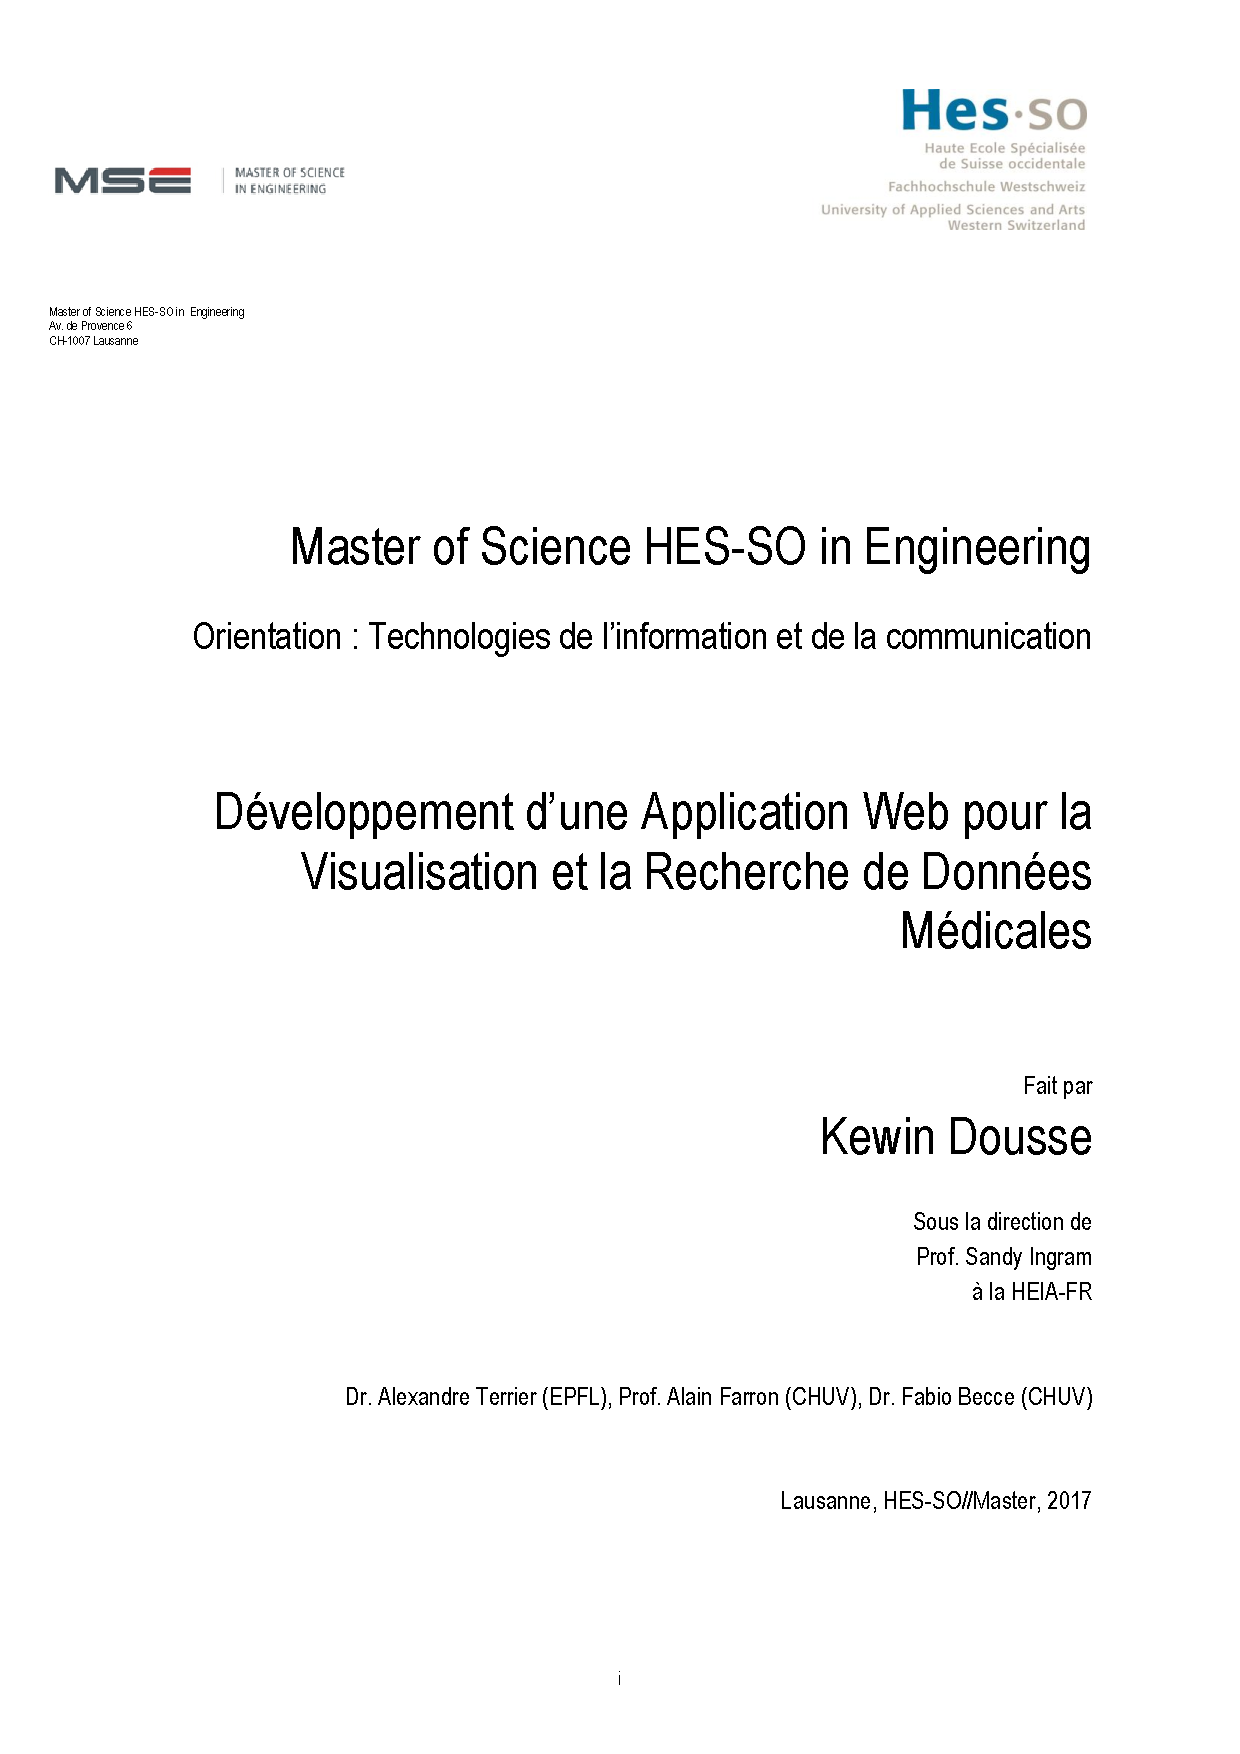
\includepdf[pages={1}]{images/garde.pdf}

\def\myTitle{Développement d'une Application Web pour la Visualisation et la Recherche de Données Médicales}
\def\myName{Kewin Dousse}
\def\myUni{HES-SO}
\def\myDepartment{TIC}
\def\mySupervisors{Sandy Ingram}
\def\myExpert{?}


\begin{abstract}

Le but de ce projet est de concevoir et d'implémenter un outil d'analyse de comportement d'utilisateurs d'applications Web pour révéler les potentiels de détection de profile des personnes (préférences, centre d'intérêt, orientations et opinions) en analysant les interactions et les informations échangées avec les applications Web.

\smallskip
\noindent \textbf{Keywords.} Web, Big Data, Privacy, Profiling

\end{abstract}
\setcounter{page}{3}
\hypersetup{pageanchor=true}

\tableofcontents
\listoffigures

\chapter{Introduction}
\section{Contexte}

	En janvier 2014, l'ONG Internet Society a publié le document Digital footprints qui aborde la question de la capacité que les webtrackers ont de définir le profile personnel des usagers d'Internet. [1]
	En 2016, Michal Kosinski chercheur à Stanford révèle les possibilités de définir un profile précis simplement en analysant les préférences (likes) enregistrées dans un profile Facebook. L'étude révèle que ce type d'analyse permet de mieux connaître une personne que ses proches et même de prévoir de probables comportements avec une grande précision. De plus, lors d'événements politiques majeurs ces techniques de profiling auraient été utilisées, comme dans le cadre des campagnes pour le Brexit ou pour l'élection du président américain Trump. [2]

	Bla contexte \gls{mot}.

	Bla liste
	\begin{enumerate}
		\item Truc 1
		\item Truc 2
	\end{enumerate}

\section{Objectifs}

	Le but de ce projet est de concevoir et d'implémenter un outil d'analyse de comportement d'utilisateurs d?applications Web pour révéler les potentiels de détection de profile des personnes (préférences, centre d'intérêt, orientations et opinions) en analysant les interactions et les informations échangées avec les applications Web. L'application développée dans ce projet a pour le but de sensibiliser le public et les médias à la question du profiling sur internet.

	Bla liste
	\begin{itemize}
		\item Truc 1
		\item Truc 2
	\end{itemize}

\section{Contraintes}

	Bla liste
	\begin{itemize}
		\item Truc 1
		\item Truc 2
	\end{itemize}

\section{Méthodologie}

	Bla
\chapter{Analyse}
%%%%%%%%%%%%%%%%%%%%%%%%%
%                          %
% ----- INTRODUCTION ----- %
%                          %
%%%%%%%%%%%%%%%%%%%%%%%%%%

\section{Projet similaire}

	\subsection{Introduction}

		Afin de placer notre recherche dans les connaissances actuelles, nous nous intéressons d'abord aux recherches récentes partageant un objectif semblable au nôtre.

		Michal Kosinski se présente sur son site web\cite{michal-kosinski} comme un "psychologist and data scientist". L'étude qu'il a co-rédigée à l'Université de Stanford en 2016 a eu un impact important sur le monde académique et même industriel, en montrant les possibilités techniques ouvertes par la récolte de données simples d'utilisateurs : les "likes" Facebook.

		Il est montré qu'avec un peu plus de 300 "likes" tirés une personne, il est possible de définir avec une précision remarquable (mieux que son époux/épouse) des traits psychologiques, ainsi que d'autres caractéristiques personnelles.

	\subsection{Résumé}

		Une enquête a été menée auprès d'une population variée de personnes possédant un compte Facebook. Les données concernant leurs "likes" ont été récoltées, ainsi que des données personnelles pouvant être disponible (ou non) selon le souhait de l'utilisateur sur Facebook, comme ses informations démographiques. Des tests psychologiques ont été également réalisés par une certaine partie des utilisateurs afin de pouvoir trouver des corrélations entre les pages likées et certains traits psychologiques.

		Cette enquête a rencontré un succès très large, et le nombre de personne ayant répondu à l'enquête, au moins en partie, se compte en millions.

		Les résultats présentés à la fin de l'étude sont inattendus : Michal annonce qu'il est possible de prédire certains comportements d'une personne mieux que son entourage le plus proche.

		Un des modèles crées avec les données récoltées, permet d'estimer le profil psychologique d'un participant selon cinq axes différents, en se basant sur ses likes Facebook. La figure~\ref{a-talk1} montre la précision obtenue par le modèle en fonction du nombre de likes utilisé en entrée.

		\begin{figure}[ht]
			\centering
			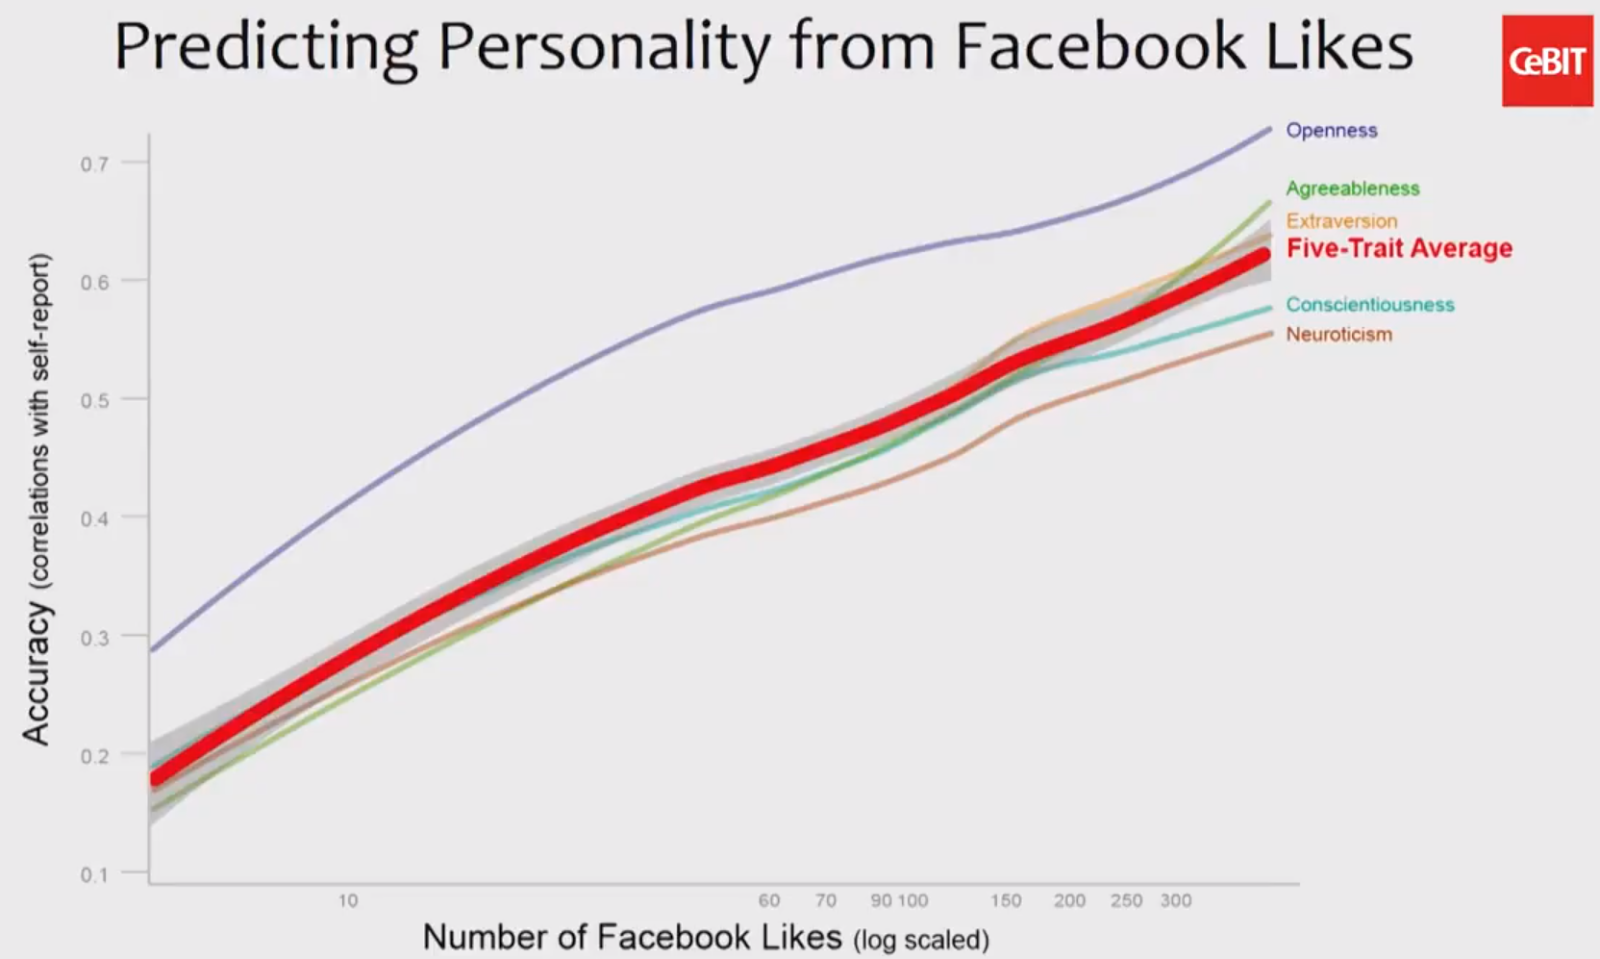
\includegraphics[width=1\textwidth]{images/analysis/talk1}
			\caption{Précision moyenne du modèle prédisant la personnalité d'un utilisateur en fonction du nombre de likes analysés\cite{kosinski-talk}.}
			\label{a-talk1}
		\end{figure}

		On remarque que la précision de la prédiction de tous les critères augmente avec le nombre de likes utilisés, ce qui n'est pas surprenant. En revanche, le tableau~\ref{a-talk-table1} montre le lien entre le nombre de likes utilisés et la précision moyenne atteinte par l'algorithme, et compare ces valeurs à la précision atteinte par d'autres êtres humains.

		\begin{table}[]
			\centering
			\begin{tabular}{lll}
				         & Précision & Nombre de likes \\
				Collègue & 0.27      & 10                            \\
				Ami      & 0.44      & 80                            \\
				Famille  & 0.5       & 100                           \\
				Epoux/se & 0.58      & 250                          
			\end{tabular}
			\caption{Précision atteinte par type de relation avec une personne, et nombre de likes nécessaires au modèle pour égaler sa précision}
			\label{a-talk-table1}
		\end{table}

		On peut voir que la précision de la prédiction de l'algorithme surpasse celle même l'époux/se d'une personne avec 250 likes, ce qui se trouve être légèrement au-dessus du nombre de likes moyen par personne, qui est de 227.

		Les possibilités de prédiction du modèle ne se limitent pas à une simple personne, et les possibilités sont nombreuses. Par exemple, Michal montre qu'il est possible de montrer une corrélation entre les visiteurs d'un certain site web, et une tendance vers certains traits psychologiques. La figure~\ref{a-talk2} montre la personnalité moyenne estimée des visiteurs du site web ```deviantart.com''' par rapport à la moyenne de tous les utilisateurs.

		\begin{figure}[ht]
			\centering
			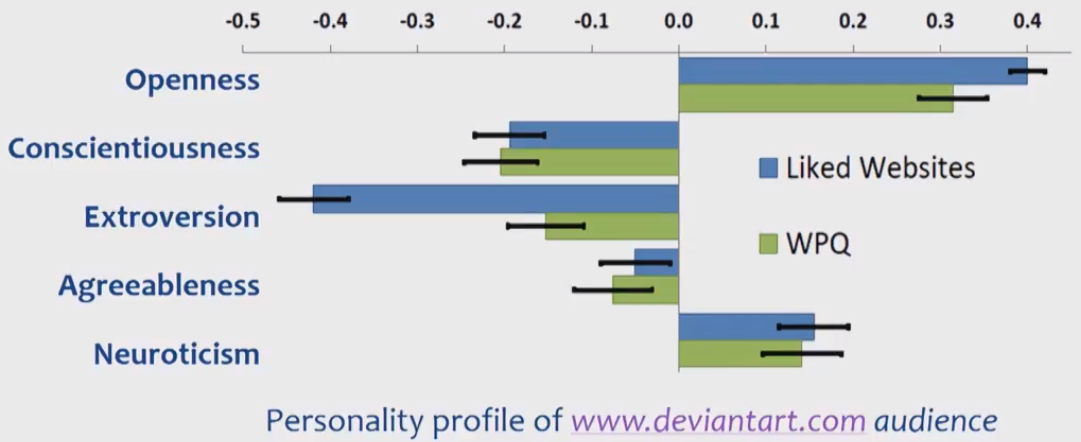
\includegraphics[width=1\textwidth]{images/analysis/talk2}
			\caption{Déviation de la personnalité moyenne estimée d'un visiteur régulier du site ```deviantart.com''' selon les cinq axes psychologiques employés\cite{kosinski-talk}.}
			\label{a-talk2}
		\end{figure}

		Ces corrélations ne sont que quelques exemples parmi un très large éventail de possibles corrélations que le modèle est capable de mettre en lumière. Les implications de telles découvertes sont massives : Il serait par exemple possible de déterminer si un utilisateur sera réceptif ou non à un certain type de publicité, par exemple. Ce genre de problématique touche à plusieurs domaines et n'est pas exactement de notre ressort ici : Des principes éthiques sont en jeu, et le sujet devient de plus en plus délicat. Mais une chose est certaine : Des likes Facebook peuvent révéler énormément d'informations.

	\subsection{Données}

		La quantité de données amassée par l'étude est massive. Non seulement en quantité d'utilisateurs, mais également en diversité de données. Michal Kosinski a mis en place le site web "myPersonnality Project"\cite{mypersonnality} permettant de partager cette source de données avec d'autres chercheurs. Les données comprennent, entre autres :

		\begin{itemize}
			\item Scores de personnalité selon la méthode BIG5 de >3 millions de personnes
			\item Données démographiques de >4 millions de personnes
			\item Localisation géographique de >1.5 million de personnes
			\item Vues politiques de >500'000 personnes
			\item Likes Facebook de >19 millions de personnes
		\end{itemize}

		Le type de données présenté ici n'est qu'un sous-ensemble restreint de l'ensemble des tables présentées, bien qu'il s'agisse ici des données comprenant le plus d'entrées au total.

	\subsection{Acquisition}

		Bien que l'objectif du site web soit de partager l'accès à cette énorme base de données, l'accès à celle-ci est loin d'être aisé. Tout d'abord, Kosinski ne met ces données à disposition que de milieux académiques, il interdit l'utilisation de ces données à des fins commerciales.

		Cependant l'accès n'est pas donné pour autant : Une demande d'accès est à lui envoyer, comprenant une présentation du projet et de ses buts par le biais d'un mail ainsi que le remplissage et l'enregistrement du projet de recherche sur des sites spécialisés.

		Cette étape ne semblait constituer qu'une marche nécessitant un temps restreint, mais un prérequis à l'envoi d'une demande d'accès à la base de données est l'approbation de l'"IRB" (Institutional Review Board), ce qui correspond à un comité d'éthique.

	\subsection{Conclusion}

		Etant donné les délais estimés de l'envoi de la demande à un comité d'éthique responsable puis de la demande d'accès aux données à Kosinski, nous avons écarté cette source de données de la liste principale du projet car nous n'avions pas l'assurance de disposer des données à temps pour la suite de l'étude. Bien qu'il s'agisse certainement d'un ajout conséquent aux données amassées par le projet, nous ne pouvons pas nous permettre de mettre en péril tout l'agenda du projet sur cette source de données.

		Bien que cette base de connaissance ait pu être utile, notre étude va changer de direction. Nous décidons de baser la recherche sur des données que nous récupérerons nous-même.

\section{Outils de tracking}

	\subsection{Trackers}

		Un tracker est un serveur contacté lors du chargement d'une page web par un utilisateur. De nos jours, les pages web sont souvent constituées de contenu provenant de plusieurs serveurs ou domaines différents. Il n'est pas rare qu'une seule page web fasse appel à plus d'une dizaine de domaines différents pour charger une seule page. La figure~\ref{a-nbdomains} montre l'évolution du nombre moyen de domaines contactés pour le chargement d'une seule page web, sur les 1'000 sites web les plus visités mondialement.

		\begin{figure}[h]
			\centering
			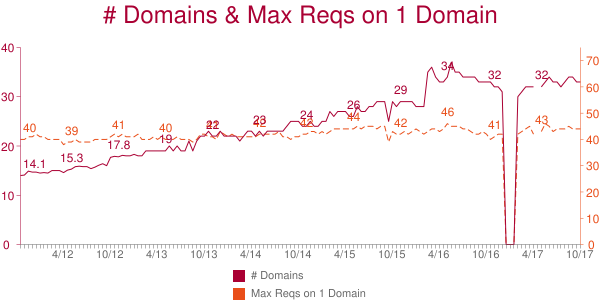
\includegraphics[width=1\textwidth]{images/analysis/nbdomains}
			\caption{Nombre moyen de domaines contactés au chargement d'une page web\cite{nbdomains}.}
			\label{a-nbdomains}
		\end{figure}

		Bien qu'une partie des domaines soient nécessaires à contacter afin de charger du contenu indispensable à la page, une partie d'entre eux ne sert également qu'à des fins statistiques ou publicitaires. Par exemple, ceux-ci peuvent récupérer des informations sur l'utilisateur et son navigateur afin de lui proposer des publicités ciblées sur ses intérêts. Cette pratique est aujourd'hui courante, comme le montre la prochaine sous-section.

	\subsection{Marché}

		Etant donné que nous nous intéressons aux données des utilisateurs récupérées lors de la navigation Web, nous cherchons à connaître quels sont les plus grand trackers sur le web.

		La figure~\ref{analytics-usage} montre la part de marché qu'occupe Google Analytics ainsi que ses compétiteurs sur les sites web Suisses.

		\begin{figure}[!h]
			\centering
			\subfloat[Utilisation de services d'analyse et de tracking\label{a-analytics-usage1}]{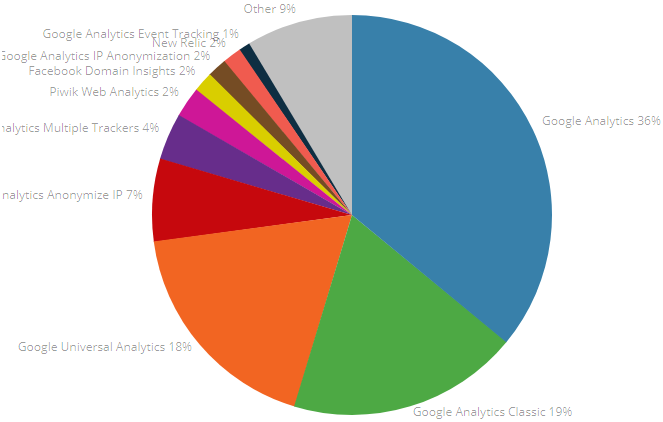
\includegraphics[width=0.45\textwidth,valign=t]{images/analysis/analytics-usage1}}
			\subfloat[Utilisation de services de mesure d'audience\label{a-analytics-usage2}]{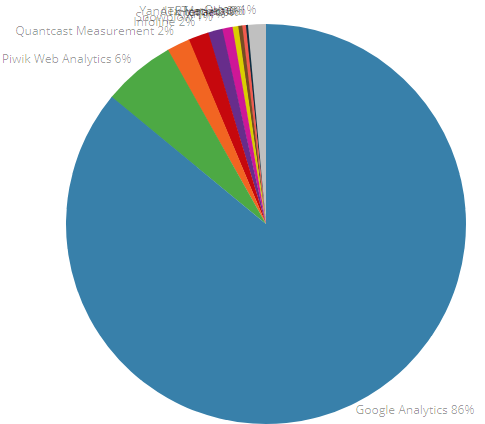
\includegraphics[width=0.45\textwidth,valign=t]{images/analysis/analytics-usage2}}
			\caption{Marché occupé par Google Analytics dans les domaines d'analyse, de tracking et de mesure d'audience sur le Web.}
			\label{analytics-usage}
		\end{figure}

		Nous pouvons calculer grâce au premier graphique que l'ensemble des produits de Google, y compris Google Analytics et ses versions proches, représentent plus de 83\% des installations de solutions dans le domaine de l'analyse et du tracking. De plus pour la sous-catégorie du marché de la mesure d'audience uniquement, Google Analytics a lui seul représente 86\% d'installations sur le Web.

		\begin{figure}[ht]
			\centering
			
\includegraphics[width=0.4\textwidth]{images/analysis/analytics}
			\caption{Logo de la solution Google Analytics\cite{analytics}.}
			\label{a-analytics}
		\end{figure}

		Il est donc de plus en plus évident que s'intéresser aux fonctionnalités de Google Analytics est intéressant pour les buts du projet. Nous souhaitons nous poser la question du risque encouru par les utilisateurs en se connectant sur un site web utilisant Google Analytics. Quelles informations sont prélevées ? Lesquelles sont envoyées ? Les données sont-elles anonymisées ?

	\subsection{Google Analytics}

		Google Analytics se présente comme une solution d'analyse de statistiques d'utilisateurs dans le but d'améliorer les résultats des sites web sur lesquels il est installé. Ce produit étant totalement gratuit pour les PME, il est aujourd'hui très répandu sur le net et particulièrement en Suisse\cite{analytics-usage}.

\section{Extensions de navigateur}

	\subsection{Introduction}

		Au vu de l'objectif du projet qui est à la fois de récolter des données tout en montrant un feedback à l'utilisateur, l'extension pour navigateurs est le moyen le plus facile à la fois pour nous de distribuer notre code, et pour les utilisateurs de l'installer. Cependant, de nombreuses extensions dont le but est de montrer des statistiques sur la navigation de l'utilisateur existent déjà. L'objectif n'est donc pas seulement d'implémenter les mesures adéquates pour notre étude, mais également de fournir des fonctionnalités à l'utilisateur novatrices afin que l'extension se démarque des concurrents.

		Une analyse des extensions existantes est donc requises afin de prendre des décisions sur la direction que vont prendre les fonctionnalités implémentées.

	\subsection{Etat de l'art}

		Nous nous intéressons aux extensions disponibles pour deux des navigateurs les plus utilisés : Google Chrome, et Mozilla Firefox. Chaque navigateur possède son propre éventail d'extensions, bien que parfois certaines se retrouvent disponibles dans les deux catalogues. Chrome Web Store\cite{chromewebstore} est le catalogue officiel d'extensions pour Google Chrome, et Modules Firefox\cite{modulesfirefox} est celui correspondant à Mozilla Firefox. Quelques recherches avec des mots-clé adaptés sur chaque catalogue vont nous fournir les extensions les plus populaires pour un thème semblable aux nôtre.

		\subsubsection{timeStats}

			timeStats\cite{timestats} est une extension disponible pour Google Chrome. La figure~\ref{a-timestats} montre comment l'extension se présente via une image montrée sur le Google chrome Store.

			\begin{figure}[h]
				\centering
				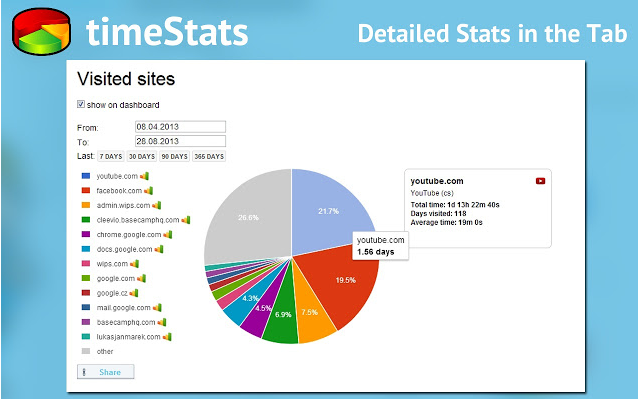
\includegraphics[width=0.6\textwidth]{images/analysis/timestats}
				\caption{Image de présentation de timeStats\cite{timestats}.}
				\label{a-timestats}
			\end{figure}

			Cette extension se focalise sur la visualisation du temps passé sur les différents sites web, parfois regroupés en domaines. La plupart des informations représentées sont le temps passé, et l'extension s'organise en plusieurs pages permettant de voir des visualisations différentes. On remarque la présence de plusieurs types de graphiques (en ligne, en secteurs) adaptés à la mesure affichée. timeStats est disponible pour Google Chrome uniquement.

		\subsubsection{Ghostery}

			Ghostery est une extension Google Chrome qui possède également sa propre page web en dehors du catalogue. La figure~\ref{a-ghostery} montre la page d'accueil du site ``ghostery.com'', qui est le domaine officiel de l'extension listée sur Google Chrome.

			\begin{figure}[h]
				\centering
				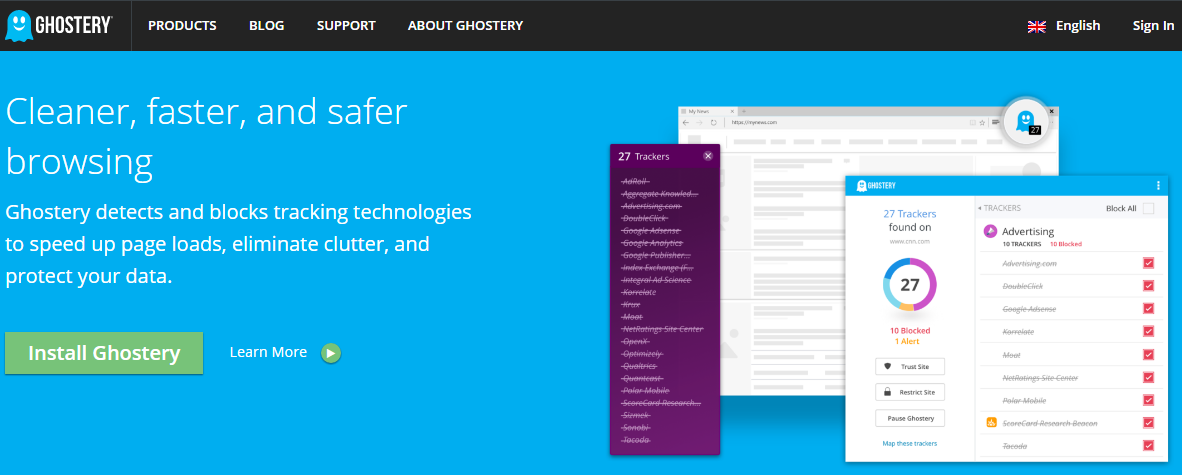
\includegraphics[width=0.8\textwidth]{images/analysis/ghostery}
				\caption{Page d'accueil de Ghostery\cite{ghostery}.}
				\label{a-ghostery}
			\end{figure}

			Ghostery semble donc se concentrer sur la détection et le blocage des informations envoyées aux trackers tiers lors de la navigation. Quelques options de personnalisation y sont présenter, comme la possibilité d'autoriser des trackers particuliers, ou des domaines choisis.

		\subsubsection{Privacy manager}

			Privacy manager se montre comme une extension permettant la gestion de mécaniques liées à la préservation de la vie privée. La figure~\ref{a-privacymanager} montre l'interface principale utilisée par l'extension.
			Bien que certaines options existent pour la protection de la vie privée, presque la moitié les options activables n'ont pas directement à faire avec la vie privée, et sont plutôt des désactivation ou activations de fonctionnalités de productivité.

			\begin{figure}[h]
				\centering
				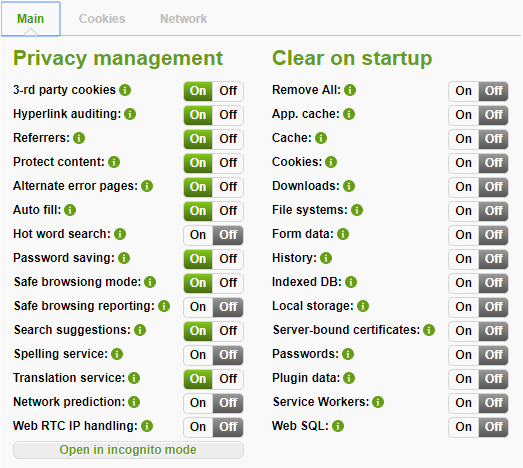
\includegraphics[width=0.5\textwidth]{images/analysis/privacy-manager}
				\caption{Interface de base de Privacy manager\cite{privacymanager}.}
				\label{a-privacymanager}
			\end{figure}

		\subsubsection{TheGoodData}

			TheGoodData remplit à priori la même mission que Ghostery, mais propose des outils légèrement différents, et son thème est centré sur l'utilisation de la valeur des données de navigation pour une bonne cause. Un tableau de bord montré à la figure~\ref{a-thegooddata} permet de se renseigner sur l'état actuel de sa navigation avec des analyses basiques sur les dangers trouvés.

			\begin{figure}[h]
				\centering
				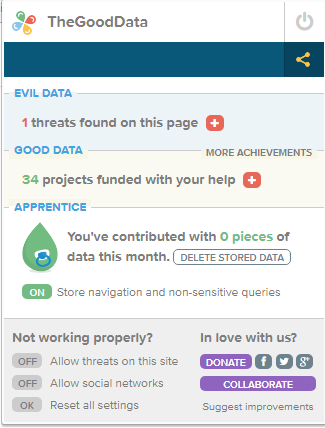
\includegraphics[width=0.4\textwidth]{images/analysis/thegooddata}
				\caption{Interface de TheGoodData\cite{thegooddata}.}
				\label{a-thegooddata}
			\end{figure}

		\subsubsection{Noiszy}

			\begin{figure}[h]
				\centering
				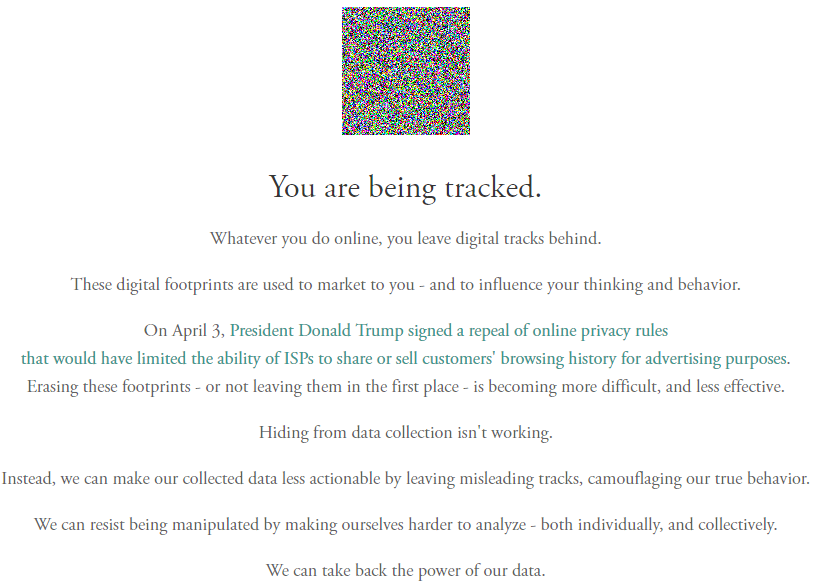
\includegraphics[width=0.9\textwidth]{images/analysis/noiszy}
				\caption{Premier paragraphe de la page web de Noiszy\cite{noiszy}.}
				\label{a-noiszy}
			\end{figure}

			Noiszy cherche quand à lui à brouiller les pistes des trackers existants, sans les bloquer. Son hypothèse de base est qu'il est presque impossible de dissimuler complètement ses "Digital Footprints", et que la meilleure solution est de tenter de les brouiller en les "falsifiant", par exemple en envoyant des données erronées aux trackers, ou en quantité trop élevées.
			La figure~\ref{a-noiszy} montre le premier paragraphe de présentation de Noiszy, présent sur leur site web.

		\subsubsection{Privacy Badger}

			Privacy Badger est une extension développée par l'EFF\cite{eff}. Disponible à la fois sur Google Chrome et Mozilla Firefox, cette extension a également comme objectif de contrôler l'envoi de données à des trackers.
			Plutôt que de strictement bloquer toute requête, cette extension laisse à l'utilisateur décider quel niveau de danger représenter chaque tracker, et adapte son comportement entre un blocage total, la retenue de certaines informations ou aucune action entreprise pour chaque tracker détecté.
			La figure~\ref{a-privacybadger} montre l'interface de l'application une fois celle-ci installée. On peut y voir les lignes de présentant chacune un tracker, et la possibilité de définir son niveau de danger, et par conséquent l'action appropriée associée.

			\begin{figure}[h]
				\centering
				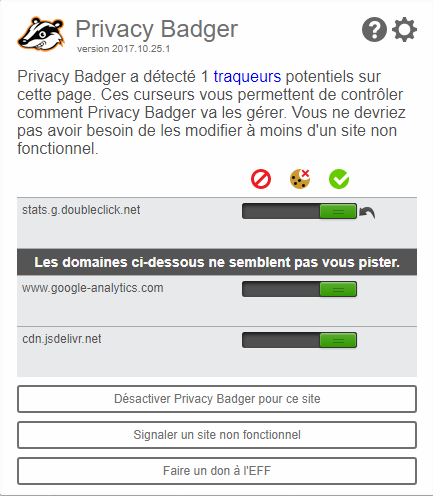
\includegraphics[width=0.5\textwidth]{images/analysis/privacybadger}
				\caption{Contrôle des actions face aux trackers de Privacy Badger\cite{privacybadger}.}
				\label{a-privacybadger}
			\end{figure}

		\subsubsection{Kraken.me}

			Kraken.me est une extension de navigateur, mais également une application pouvant s'installer sur smartphone. Cette application analyse le flux de données de certains services comme Facebook, Twister, LinkedIn et encore d'autres. L'objectif est ici de donner à l'utilisateur une vue sur ses propres données, et la manière que celles-si sont utilisées par les applications.
			La figure~\ref{a-krakenme} montre le modèle présenté par le site web.

			Cette application est probablement une des plus semblable à l'objectif général de notre projet, il serait donc intéressant de voir quels ont été les débouchés de cette étude. Notons que la plupart de l'activité de celle-ci ainsi que de l'outil semblent avoir cessé en 2014.

			\begin{figure}[h]
				\centering
				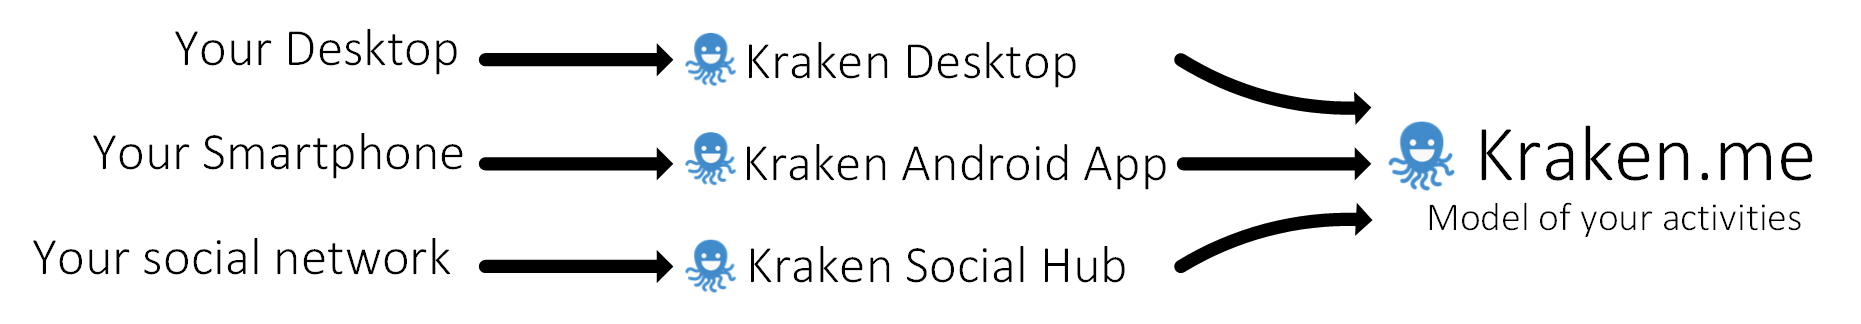
\includegraphics[width=0.8\textwidth]{images/analysis/krakenme}
				\caption{Flux de données de Kraken.me\cite{krakenme}.}
				\label{a-krakenme}
			\end{figure}

	\subsection{Conclusion}

		Après avoir dressé une liste des extensions de navigateur les plus populaires et utilisés, nous pouvons prendre position sur les fonctionnalités que notre extension va posséder afin de se démarquer et de répondre à la problématique de l'étude. Nous allons choisir les fonctionnalités que nous estimons avoir un impact pour la sensibilisation du public aux traces que les internautes laissent, et des informations que nous pouvons en retirer. Ainsi, le plug-in se concentrera sur les deux aspects suivants :

		\begin{itemize}
			\item Détection et mise en lumière des différents trackers présents sur les pages visitées par l'utilisateur.
			\item Tentative de reconstitution du profil de l'utilisateur à partir de la fréquence de la visite des pages web et de leur contenu.
		\end{itemize}

\section{Analyse de texte}

	Nous allons utiliser le contenu des pages pour trouver des informations sur les centres d'intérêt de l'utilisateur. Pour ceci, nous avons besoin d'analyser et de tenter de comprendre le contenu des pages.

	\subsection{Keyword extraction}

		Le keyword extraction est le nom donné à un algorithme dont le but est de ressortir, parmi les mots d'un document, quels en sont les mots les plus représentatifs, ou les plus expressifs. Cette opération ne se fait généralement pas sur un seul document, mais sur un ensemble de documents, appelé corpus. Il s'agit d'une sous-catégorie des algorithmes de \gls{NLP}.

		Dans notre cas, les techniques de keyword extraction que nous prenons en compte sont les techniques dites "non supervisées". Cela signifie que nous n'avons pas d'information à priori sur quels sont les mots qui vont être potentiellement importants dans le texte, et que nous laissons une complète liberté à l'algorithme.

		Parmi les techniques de keyword extraction, on peut citer les plus connus : \gls{TF-IDF}, TextRank et \gls{RAKE}. Etant donné que ces algorithmes fonctionnent de manière semblable, il a fallu se pencher sur des études montrant leur efficacité afin de décider lequel de ceux-ci nous allons utiliser.

		\subsubsection{Recherche}

			Etant donné qu'il s'agit ici d'entraîner des modèles à l'aides d'algorithmes non-supervisés, il n'existe pas de méthode efficace cartésienne pour prouver que nous obtenons des bons résultats à l'aide des modèles générés. Nous ne cherchons ici une vérité absolue, mais nous voulons trouver des modèles dans les pages parcourues par l'utilisateur. Les publications étudiées font donc également souvent appel à un jugement humain afin de définir si une méthode est adaptée ou non.

			Un total de trois ressources a été étudié pour baser notre choix de la technique de keyword extraction à utiliser.

			\paragraph{Première étude}
			
				La première source\cite{text-analysis-src4} présente un cas concret où on cherche à classifier une série de documents connus à l'avance, présentant des sujets communs. Le but est de créer un modèle capable de reconnaître le thème de nouveaux documents  en créant un modèle à partir d'une liste de documents connus. Bien que la comparaison soit faite entre TF-IDF, RAKE et TextRank, le cas ici assez différent du nôtre. En effet, le cas décrit ici cherche à entraîner un modèle de manière supervisée. 

				L'ensemble des documents en entrée est une liste de documents lus par l'auteur de l'article durant les 6 dernières années. Après avoir testé les trois algorithmes et comparé les différents résultats, la conclusion est que pour ce cas, TextRank et RAKE sont les algorithmes préférables. Le reproche est fait à TF-IDF de classer trop bas certains mots qui apparaissent dans de nombreux documents. Par exemple, nous savons que l'auteur a lu beaucoup de document sur JavaScript, et donc TF-IDF met un poids très faible à ce mot.

				Cette conclusion est sensée, mais ce problème ne s'applique pas à notre cas. En effet, nous cherchons spécifiquement à avoir un éventail très large de pages afin d'éviter ce genre de cas. Également, notre entraînement ne sera pas supervisé, nous ne pourrons donc pas évaluer les résultats finaux de cette manière.

			\paragraph{Deuxième étude}

				La deuxième étude\cite{text-analysis-src5} se penche sur l'extraction automatisée et non supervisée de keywords, ce qui est cette fois très proche de notre cas. Cette fois-ci, la publication se base sur des méthodes statistiques pour tenter de prédire quel est l'algorithme le plus efficace pour le keywords extraction en comparant les résultats de ceux-ci avec l'avis d'humains auxquels ont demande d'exécuter la même tâche.

				Sont comparées ici la méthode TF-IDF ainsi que certaines de ses variantes, et plusieurs méthodes basées sur l'utilisation de graphes (référées simplement comme "Graph-based methods" à plusieurs endroits du texte).

				Après une comparaison des résultats de chaque méthode avec les résultats trouvés par des humains, il est conclu que "Our results on the human transcripts show that the simple TFIDF based method is very competitive"\cite{text-analysis-src5}. Certaines variantes de TF-IDF où la position des mots dans une phrase ajoute un poids aux mots offre des scores très comparables à la méthode de base, mais les autres techniques ont montré des résultats plus faibles.

			\paragraph{Troisième étude}

				Le troisième document\cite{text-analysis-src6} est en réalité une question posée sur le site Quora, où des experts ont proposé une réponse à la question "What are the best keyword extraction algorithms for natural language processing and how can they be implemented in Python?".

				Les trois méthodes populaires \gls{TF-IDF}, TextRank et \gls{RAKE} sont à nouveau citées, mais il ressort que RAKE et TF-IDF semble être consensuellement les méthodes les plus efficaces.

			À la fin de l'analyse de ces sources, nous choisissons d'utiliser l'algorithme TF-IDF, qui semble être à la fois efficace et adapté à notre cas.

		\subsection{TF-IDF}\label{analyse-tfidf}

			TF-IDF est une méthode attribuant un poids à chaque mot de chaque document d'un corpus. Ce poids mesure l'importance relative du mot dans ce document. Le nom "TF-IDF" signifie "Term Frequency - Inverse Document Frequency". Le poids final d'un mot dans un document se calcule en prenant en compte uniquement deux mesures :
			\begin{description}
				\item[TF] Term Frequency : La quantité d'apparition de ce mot dans ce document
				\item[DF] Document Frequency : Le nombre de documents dans lesquels ce mot apparaît
			\end{description}

			Le score final d'un mot multiplie le TF d'un mot à l'inverse de son DF. Cela signifie que pour avoir une grande importance dans un document, un mot sera typiquement :
			\begin{itemize}
				\item Présent de nombreuses fois dans ce document
				\item Présent dans très peu d'autres documents
			\end{itemize}

			Le calcul des poids se fait sur l'ensemble du corpus en une fois, car il nécessite que l'on connaisse le nombre d’occurrences de chaque mot dans l'entièreté du corpus de documents. Il n'est donc pas possible de mettre à jour les poids de manière "online" en utilisant ce modèle.

	\subsection{Topic Modeling}

		Le topic modeling est un exercice différent de celui du keyword extraction. Nous ne cherchons plus ici à trouver les meilleurs mots parmi des textes, mais nous cherchons à les regrouper afin d'en former des thèmes, ou "topic"s.

		Le but est cette fois de déterminer par des méthodes statistiques quels sont les thèmes communs à plusieurs documents, nous permettant ainsi de les regrouper. Ceci part du principe que nous appliquons l'apprentissage de l'algorithme sur un corpus de documents qui contient des textes qui ont effectivement des thèmes en commun. Ce qui est sans doute notre cas lorsque notre corpus est composé de pages web visitées par des utilisateurs.

		\subsubsection{Recherche}

			Etant donné que nous sommes dans le même cas que TF-IDF, à savoir en recherche d'un algorithme pour le cas d'un apprentissage non supervisé, la plupart des méthodes tentant de comparer des modèles se basent sur des mesures empiriques. Le jugement humain est à nouveau indispensable dans ce cas pour déterminer de l'adéquation d'un algorithme ou non avec les buts recherchés.

			Nous recherchons ici une méthode relativement populaire car nous allons nous baser sur une librairie l'implémentant déjà. Il aurait été possible de développer nous-même ce module, mais nous avons estimé que les efforts à déployer pour ce faire étaient trop élevés pour justifier le temps passé.

			Après quelques recherches sur le web, les méthodes les plus populaires semblent être LSA, pLSA et LDA\cite{stanford-topicmodel}. Cependant, les études comparatives entre ces méthodes semblent très rares, et les seules sources trouvées furent des déclarations de chercheurs. Voici les ressources ayant contribué au choix de la méthode :

			\paragraph{Première source} 

				La première source comparant ces algorithmes est une réponse à une question posée sur le site web Quora\cite{quora-topicmodel}. À la question "What's the difference between Latent Semantic Indexing (LSI) and Latent Dirichlet Allocation (LDA)?", la réponse votée le plus positivement par un consultant en NLP conclut "In practice, LSI is much faster to train than LDA, but has lower accuracy.".

			\paragraph{Seconde source}

				La deuxième source est une question posée sur le site Reddit, intitulée "LSA vs pLSA vs LDA"\cite{reddit-topicmodel}. L'auteur demande la différence et les avantages de chaque méthode, et une réponse résume chaque algorithme en une simple ligne :
				\begin{quote}
LSA -> uses SVD, and as a result the topics are assumed to be orthogonal.

pLSA -> Treats topics as word distributions, uses probabilistic methods, and topics are allowed to be non-orthogonal.

LDA -> similar to pLSA, but with dirichlet priors for the document-topic and topic-word distributions. This prevents over-fitting, and gives better results.
				\end{quote}

				Semblablement, le modèle LDA semble primer dans l'avis sur la qualité des résultats. Après une recherche de librairies, il se trouve que LDA possède une implémentation en Python, dans une librairie nommée gensim. Nous nous arrêtons donc sur ce choix, comme le modèle semble à la fois précis et adapté à notre cas d'utilisation avec Python.

	\subsection{LDA}\label{analyse-lda}

		LDA (de l'anglais Latent Dirichelet Allocation) est un modèle de topic modeling, et va nous permettre de révéler des topics relatifs aux pages visitées par les utilisateurs. Ici, un topic est définit par une liste de mots, et un poids associé à chaque mot pour le topic.

			La génération d'un modèle LDA prend plusieurs paramètres en entrée, mais le plus important pour nous est de définir un nombre de topics que nous souhaitons voir en sortie. On fixe ce nombre de topics, puis on lance l'apprentissage du modèle sur l'ensemble du corpus de documents, opération que peut durer plusieurs heures.

			À la fin de l'apprentissage, nous sommes en possession d'un modèle que nous pouvons questionner de plusieurs manières, par exemple :
			\begin{itemize}
				\item Quels sont les mots les plus contribuant à un topic ?
				\item Quels sont les topics les plus probables pour un document ?
			\end{itemize}

			Nous allons donc par exemple utiliser le modèle afin d'assigner des topics au contenu d'URLs, et ainsi tenter de trouver quels sont les thèmes communs aux pages visitées par un utilisateur.
\chapter{Conception}
%%%%%%%%%%%%%%%%%%%%%%%%%%
%                          %
% ----- INTRODUCTION ----- %
%                          %
%%%%%%%%%%%%%%%%%%%%%%%%%%

\section{Introduction}

	\subsection{Idée}

		Le but recherché de l'outil est de sensibiliser les utilisateurs aux informations que ceux-ci dévoilent potentiellement en naviguant sur le web. Pour ce faire, nous avons besoin d'amasser des données sur leurs habitudes de navigation afin de les analyser.

		Ces données seront centralisées sur un serveur afin que nous puissions lancer des traitements sur l'ensemble des données plus tard dans le but de tenter de révéler des tendances, habitudes ou corrélations entre les données.

		De plus, nous souhaitons également offrir un service direct à l'utilisateur afin que celui-ci ait un bénéfice à installer l'extension et nous autoriser à accéder à ces données. Nous allons lui montrer via une interface web les données que nous avons pu amasser sur sa navigation depuis l'installation du plug-in, au travers de plusieurs pages et visualisations.

		Nous souhaitons également que les données récupérées ne puissent pas être utilisées pour reconnaître une personne particulière. C'est pourquoi le plug-in ne nécessite aucune connexion avec un compte externe, et ne demande pas information directement divulgatrice d'une identité.

		Nous pouvons ainsi résumer les caractéristiques principales du plug-in en quelques points.

		Le plug-in :
		\begin{itemize}
			\item Récupère les informations de navigation de l'utilisateur
			\item Envoie ces informations de manière anonyme à un serveur centralisé
			\item Propose une visualisation des données récoltées et calculées sur l'utilisateur
		\end{itemize}

	\subsection{Architecture}

		Le projet dans son ensemble requiert le développement d'un minimum de deux parties différentes :

		\begin{itemize}
			\item Une extension pour navigateur afin de récupérer et d'envoyer les données
			\item Un serveur recevant les données des extensions installées
		\end{itemize}

		Une troisième partie s'occupant de l'interface utilisateur est également à prévoir, celle-ci pouvant se situer autant dans l'extension que sur le serveur. La décision est finalement prise d'héberger l'interface utilisateur sur un différent serveur, auquel se connecte l'interface lorsque l'utilisateur souhaite accéder à sa page.

		\begin{figure}[h]
			\centering
			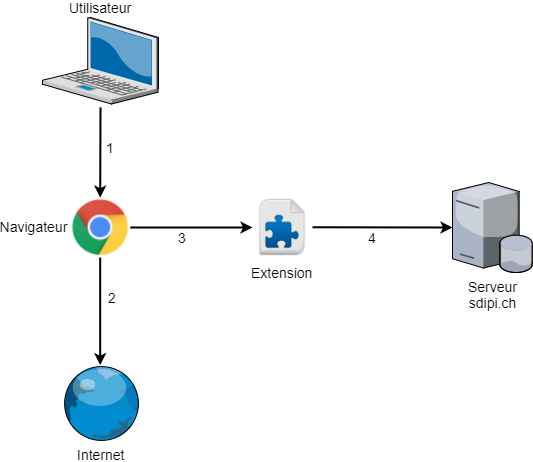
\includegraphics[width=0.8\textwidth]{images/design/intro/architecture}
			\caption{Flux de données de l'extension.}
			\label{d-architecture}
		\end{figure}

		La figure \ref{d-architecture} schématise la récolte de données effectuée par l’extension.
		\begin{enumerate}
			\item L'utilisateur entre une URL dans son navigateur
			\item Le navigateur accède à la ressource concernée
			\item Le navigateur transmet au plug-in les informations concernant la navigation
			\item Le plug-in contacte le serveur SDIPI pour lui transmettre les informations
		\end{enumerate}

	\subsection{Données}\label{d-donnees}

		Les possibilités de récolte de données depuis une extension de navigateur sont extrêmement nombreuses. Nous allons cependant nous concentrer sur l'amassage de données utiles à l'étude, et qui ne représentent pas une menace à l'intimité de l'utilisateur. Nous devons donc nous limiter à un set de données adéquat.

		Voici les différents types d'informations que nous récoltons, et à quelles fins chaque type d'information est utilisé :

		\subsubsection{Visite d'une URL}
			
			Lorsque l'utilisateur accède à une nouvelle URL dans son navigateur, qu'il s'agisse d'un clic sur un lien ou d'une entrée dans la barre d'adresse, l'extension enregistre une partie de l'URL accédée ainsi que la date d'accès. Pour des raisons de protection de la vie privée, seule une partie de l'URL est conservée et envoyée au serveur.

			\begin{figure}[h]
				\centering
				$\underbrace{\texttt{https://www.google.ch/search}}_{\text{Partie conservée}}$\texttt{?q=Recherche+test}
				\caption{Exemple d'URL et traitement}
				\label{d-url}
			\end{figure}

			La figure~\ref{d-url} montre que tous les paramètres de la requête ne sont pas conservés. Seuls le protocole (\texttt{http} ou \texttt{https}), le nom de domaine, l'éventuel numéro de port ainsi que le chemin d'accès à la ressource sont conservés. Nous évitons ainsi la possibilité de stocker des informations sensibles comme le nom d'utilisateur, qui peut parfois se trouver dans cette partie de l'URL de certains sites web.

			De plus, nous savons déjà que certaines URLs ne seront pas utiles à notre étude. Par exemple, nous pouvons d'avance dire que les URLs menant à des pages dont le contenu est constitué de l'une de ces manières est peu adéquat à analyser :
			\begin{itemize}
				\item Du texte généré spécialement lorsque l'utilisateur est connecté à un compte, par exemple une page d'accueil d'un service
				\item De contenu principalement autre que du texte, par exemple une page mettant en avant une vidéo
				\item De contenu régénéré très fréquemment, par exemple une première page d'un site de news
			\end{itemize}
			
			Nous décidons donc de définir une liste d'URLs que nous ne prendrons volontairement pas en compte lors de l'analyse. Le but de cette liste n'est bien sûr pas d'exhaustivement ignorer les sites dont le contenu textuel est très peu fiable ou présente très peu d'intérêt, mais d'améliorer la qualité possible des résultats en écartant certains cas dont nous pouvons raisonnablement dire qui apportent des biais par rapport à la réalité.

			Ainsi, nous avons dressé une simple liste d'une dizaine de patterns d'URL que nous allons volontairement ignorer. Dans cette liste nous retrouvons des pages d'accueil de sites comme \texttt{\^{}https?://www.facebook.com/?\$} ou \linebreak
			\texttt{\^{}https?://www.twitter.com/?\$}, mais également des sites de lecture de vidéo comme \texttt{\^{}https?://www.youtube.com} et d'autres cas plus spécifiques, comme les URLs ne pointant pas vers des ressources accessibles en HTTP ou HTTPS : \texttt{\^{}(?!http)}.

		\subsubsection{Activité sur une page}

			À tout moment, l'utilisateur a probablement plusieurs onglets ou plusieurs fenêtres de navigateur ouvertes. Nous souhaitons nous intéresser à quelle page est actuellement en train d'être parcourue par l'utilisateur. À cette fin, nous détectons les événements sur la page web : Appui sur une touche, ou clic de souris par exemple. Dès lors qu'il se passe plus de 30 secondes sans aucun événement de la part de l'utilisateur, nous estimons qu'il ne regarde plus activement la page. Ce temps passé à s'intéresser à chaque page est également envoyé au serveur central toutes les 30 secondes.

		\subsubsection{Requêtes du navigateur}

			Lorsque le navigateur accède à une page web ou à d'autres moments, le navigateur doit charger des ressources qui se trouvent sur un serveur distant. Ce chargement peut prendre place pour afficher par exemple une image, un morceau de la page web elle-même, ou être demandé par un script chargé.

			Pour chaque requête que le navigateur envoie, l'extension mémorise certaines informations : 
			\begin{description}
				\item[Origine] L'extension mémorise l'URL de la page qui demande la ressource. Cette information est traitée de la même manière que décrit à la figure~\ref{d-url}.
				\item[Hôte] Toujours d'une manière identique à la figure~\ref{d-url}, l'extension mémorise également le serveur contacté.
				\item[Taille] L'extension mémorise également la taille de la requête en question, qui correspond à l'addition du contenu envoyé dans le contenu de celle-ci, ainsi que la taille des paramètres (ceux qui ne sont pas retenus par l'extension).
			\end{description}

		\subsubsection{Identificateur}

			Lors de l'installation de l'extension, un nombre aléatoire est généré pour l'installation. Cet identificateur est envoyé envoyé au serveur central en plus de chaque autre information : Elle nous est utile pour assigner chaque donnée de navigation avec un navigateur particulier.

\section{Architecture}

	\subsection{Stack technologique}

		L'ensemble des éléments constituant le projet peuvent être regroupés en 3 parties différentes où s'exécute le code.

		\begin{figure}[!h]
			\centering
			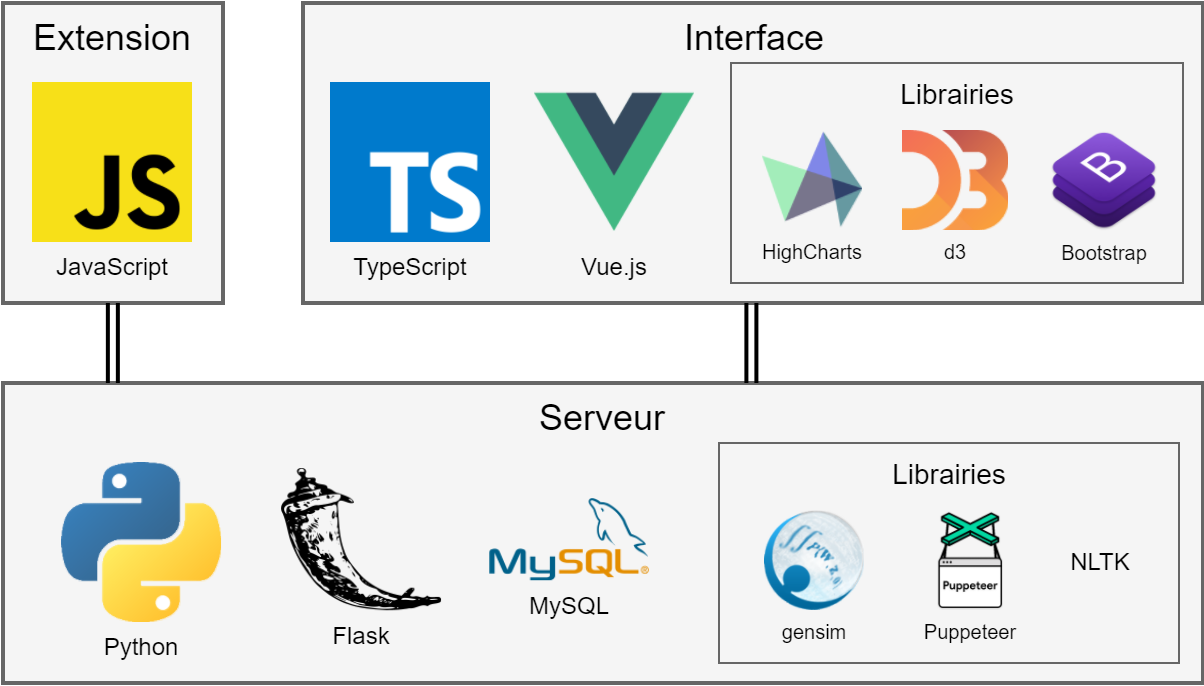
\includegraphics[width=1\textwidth]{images/design/stack}
			\caption{Technologies utilisées pour chaque partie}
			\label{d-stack}
		\end{figure}

		La figure~\ref{d-stack} montre les trois parties ainsi que les technologies utilisées dans chacune.

		\begin{itemize}
			\item L'extension comprend le code exécuté dans le navigateur du client, et qui communique avec l'API de Google Chrome afin de pouvoir récolter et envoyer les informations.
			\item L'interface comprend le code des diverses pages de visualisations montrées à l'utilisateur. On peut accéder à cette série de pages via un lien montré dans l'extension, ou par leur URL directement.
			\item Le serveur comprend le code exécuté notre machine.
		\end{itemize}

	\subsection{Extension}

		L'extension de navigateur est sans aucun doute la partie la plus simple du projet. Etant donné que nous avons décidé d'héberger l'interface utilisateur sur un serveur différent, l'extension ne va principalement s'occuper que de récupérer les données de l'utilisateur et les transmettre à notre serveur.

		Etant donné qu'une extension de navigateur n'est disponible que pour un type de navigateur à la fois, la question du support de plusieurs navigateurs s'est posée. D'après le site populaire \texttt{w3schools.com}\cite{browser-stats}, Google Chrome représente plus de 75\% des visites au moins de décembre 2017. Nous décidons donc de ne pas adapter le code de l'extension pour plusieurs types de navigateurs, car nous estimons que le gain en utilisateurs serait insuffisant pour justifier le développement supplémentaire.

		L'extension sera donc développée pour le navigateur Google Chrome, en utilisant l'API JavaScript que celui-ci met à disposition. Les fonctionnalités implémentées sont la récolte et l'envoi des types de données décrites à la section \ref{d-donnees}.

		L'extension proposera également à l'utilisateur d'accéder à l'interface grâce à un lien, ainsi que la possibilité de se "lier" ce navigateur au profil d'un autre navigateur existant, en entrant son ancien identificateur. Ceci permet à un utilisateur de profiter d'un seul profil au travers de plusieurs machines possédant l'extension, par exemple. 

	\subsection{Serveur}

		\subsubsection{Rôles}

			La partie du serveur est probablement la plus complexe du projet. Le serveur va devoir assurer le fonctionnement de plusieurs tâches clés :

			\begin{itemize}
				\item Récolte et enregistrement des données de l'extension
				\item Traitement des données utilisateurs
				\item API au service de l'interface
			\end{itemize}

		\subsubsection{Récolte}

			Avant tout traitement, le serveur doit être capable de recevoir et d'enregistrer les données des clients. Etant donné que l'extension est développée en JavaScript, les données seront transmises par HTTP au format JSON pour des raisons de simplicité.

			\paragraph{Installation du plug-in}

				Au moment où le plug-in est installé, une requête est envoyée au serveur afin de l'avertir qu'un nouvel utilisateur a installé l'extension. Le serveur génère un identifiant, l'envoie à l'extension en réponse et est désormais prêt à recevoir des information de ce nouvel identifiant.

			\paragraph{Récolte continuelle\label{d-recolte}}

				Afin que le serveur soit capable de supporter une certaine charge d'utilisateurs, il est nécessaire que celui-ci reçoive un nombre réduit de requêtes de la part des clients. Pour cette raison, l'extension ne contacte le serveur qu'une seule fois toutes les 30 secondes afin de le tenir informé des événements ayant eu lieu.

				Le serveur va donc pouvoir exposer une API simple : L'extension contactera toujours le même endpoint, et chaque requête contiendra la liste des informations concernant les événements qui se sont passés chez le client.

				Lorsque nous détectons qu'utilisateur visite une URL pour la première fois, le serveur va télécharger le contenu de cette page. Notre serveur ouvre un navigateur virtuel afin de simuler le chargement complet de la page - y compris l'exécution de scripts - et enregistre le contenu final de la page dans la base de données.

				\begin{figure}[!h]
					\centering
					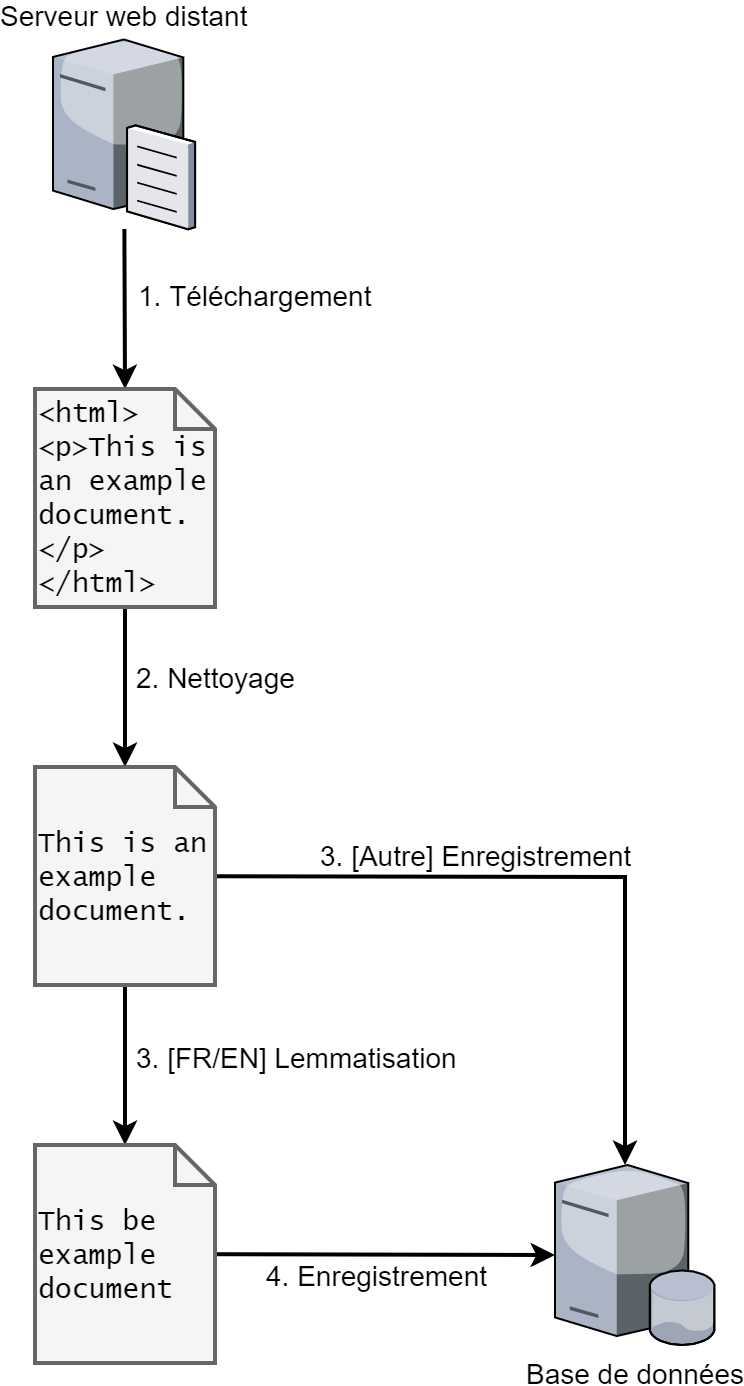
\includegraphics[width=0.5\textwidth]{images/design/data1_big}
					\caption{Téléchargement et enregistrement du contenu d'une page}
					\label{d-download-page}
				\end{figure}

				Une série d'opérations est ensuite effectuée sur le contenu de la page, afin de le rendre utilisable par les prochains algorithmes. La figure~\ref{d-download-page} montre les étapes qui entrent en compte dans le pré-traitement du contenu :

				\begin{description}
					\item[1. Téléchargement] Le serveur lance, dans un navigateur virtuel, le téléchargement de la page ainsi que l'exécution des scripts présents sur celle-ci. Une fois la page complètement chargée, on conserve le DOM de la page chargée.
					\item[2. Nettoyage] À partir du HTML de la page, on ne cherche à garder que le texte de celle-ci, sans balise. Un parseur enlève toutes les balises \texttt{<script>} et \texttt{<style>}, puis ne garde que le contenu des éléments restants.
					\item[3. [FR/EN] Lemmatisation] Un détecteur de langue nous renseigne sur la langue du texte. Si celui-ci est en anglais ou en français, nous lemmatisons chaque mot du texte. Ce processus analyse lexicalement les mots présents, et tente de ramener chaque mot à dans une forme plus simple pour le représenter. Par exemple, le temps des verbes est changé en infinitif, et les noms communs perdent leur pluriel. La liste complète des traitements effectuée est en réalité bien plus longue, et propre à la langue du texte.
					\item[3/4. Enregistrement] Si le texte n'est pas dans une langue supportée par la lemmatisation, ou après la lemmatisation du texte anglais ou français, celui-ci est enregistré dans la base de données. Tous les traitements futurs sur le contenu de la page se feront sur cette version-ci.
				\end{description}

		\subsubsection{Enregistrement}

			Le serveur se charge également de la gestion du stockage des données reçues (et calculées). Une base de données MySQL sera continuellement alimentée par les nouvelles données reçues. La base de données comprendra généralement une table par type de données à enregistrer, ainsi que des tables temporaires dans lesquelles seront placées des informations pré-calculées afin de répondre plus rapidement aux requêtes de l'interface.

		\subsubsection{Traitement des données}

			Une fois des données enregistrées, celles-ci sont traitées par différentes méthodes en fonction des besoins de l'interface. Voici le traitement que subit chaque type de données. Les traitements décrits ici ne sont pas effectués directement à la réception de données d'un client : Ils sont effectués régulièrement lorsque nécessaire.

			\paragraph{Quantité de visites}

				Deux mesures sont récoltées sur l'intérêt que peut avoir un utilisateur par rapport à une page web : Le nombre de fois que cette URL a été ouverte, et le temps passé à être actif sur la page en question. Chacune de ces informations est également datée.

			\paragraph{Contenu des pages}

				Les traitements les plus lourds que nous effectuons prennent en entrée le contenu des pages visitées.

				\begin{figure}[!h]
					\centering
					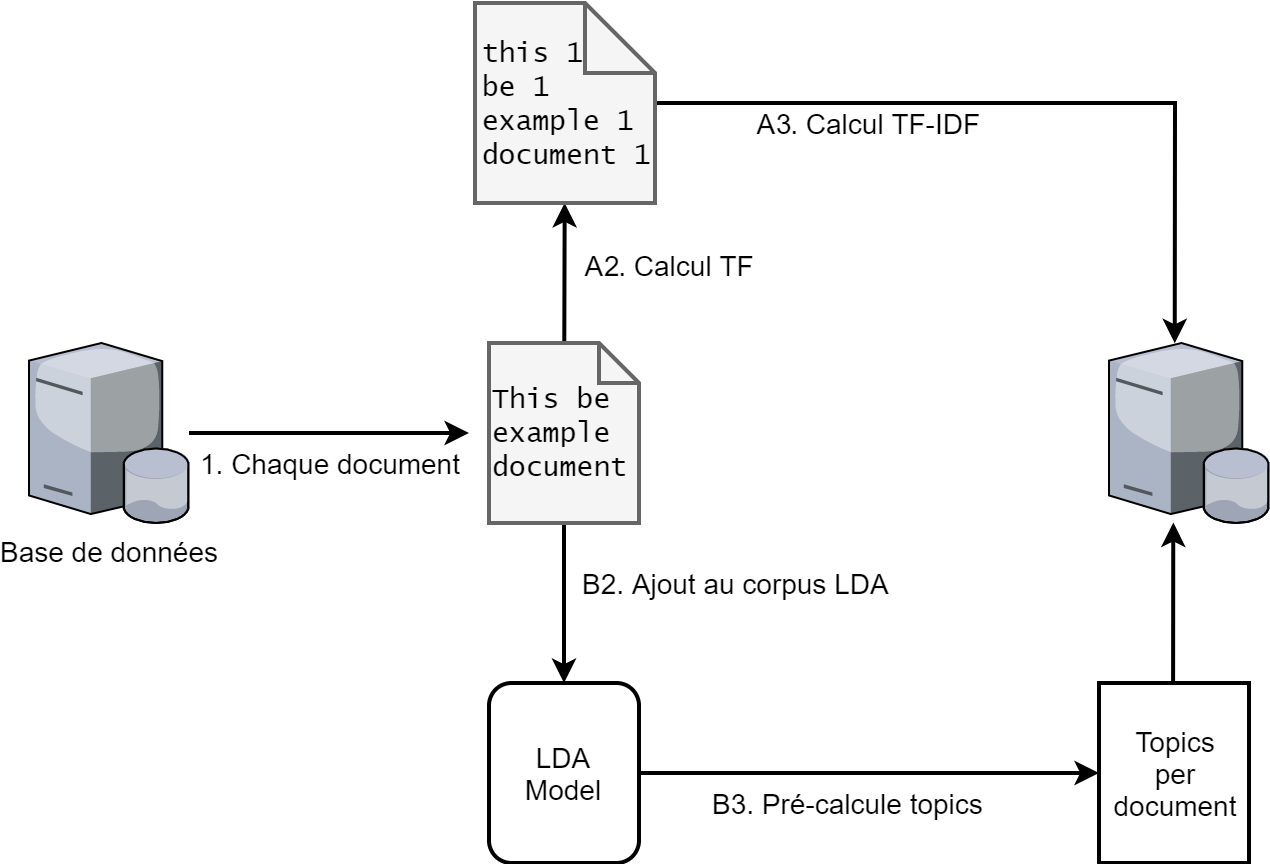
\includegraphics[width=0.8\textwidth]{images/design/traitement_offline}
					\caption{Traitements du contenu des pages}
					\label{d-traitements}
				\end{figure}

				Le contenu de la page est analysé indépendamment par deux algorithmes différents, chacun permettant de révéler un type d'information différent.

				La figure~\ref{d-traitements} montre les deux traitements effectués aux documents de la base de données.

				\begin{description}
					\item[1. Chaque document] le serveur va charger la liste entière des contenus enregistrés des pages web, obtenues comme décrites à la section \ref{d-recolte}.
					\item[A2. Calcul TF] La fréquence de chaque mot du document est calculée, puis enregistrée
					\item[A3. Calcul TF-IDF] Une fois en possession de la fréquence de chaque mot dans chaque document, le poids final TF-IDF normalisé est calculé et enregistré dans la base de données, pour chaque mot à l'intérieur de chaque document.
					\item[B2. Ajout au corpus LDA] Avant de générer un modèle, un traitement semblable à la branche A2 est effectuée pour chaque document. Une fois tous les documents chargés, on lance l'exécution de la génération du modèle LDA.
					\item[B3. Pré-calcule topics] Une le modèle entraîné, processus qui peut facilement durer plusieurs heures, il est enregistré sur le disque. Après quoi, une multitude de requêtes sont effectuées sur le modèle afin de connaître déjà quels sont les topics les plus probables pour chaque page de la base de données. On enregistre les résultats à nouveau dans la base de données. Ce pré-calcul va accélérer considérablement les traitements futurs sur la reconnaissance des topics significatifs pour un utilisateur en fonction des pages web qu'il a visité. 

				\end{description}

				\subparagraph{TF-IDF}

					TF-IDF est une méthode permettant de détecter quels sont les mots les plus importants dans un document parmi l'ensemble d'un corpus. La méthode consiste purement en l'analyse de la fréquence de chaque mot dans chaque document, et ne s'occupe absolument pas de la signification des mots.

				\subparagraph{LDA}

					LDA est un modèle qui permet de générer un nombre de sujets, thèmes ou topics, en fonction du contenu textuel d'un corpus de documents. Le modèle suppose que chaque document parle de un ou plusieurs topics, et tente de les retrouver en se basant sur la fréquence d'utilisation de ses mots en comparaison avec le reste du corpus de documents. 

			\paragraph{Requêtes du navigateur}

				Comme mentionné précédemment, quelques informations de chaque requête du navigateur du client sont enregistrées. Ces données n'ont pas besoin d'un traitement particulier.

				Etant donné que nous nous intéressons particulièrement à leur quantité, nous n'allons principalement que les compter. Cependant dû au fait de leur énorme quantité, il nous est nécessaire de pré-calculer certaines sommes avant de les servir à l'interface.

		\subsubsection{API}

			Le serveur a également le rôle de répondre aux demander de l'interface, et de lui fournir les informations nécessaire pour afficher les données du client. Ces communications se font au travers d'une série de requêtes initiées par le client.

			Une partie des données servies au client sont pré-calculées, comme la liste des topics tirés de LDA ou le poids TF-IDF des mots, et ne sont donc rafraîchies que périodiquement lorsque demandé.

			Le reste des données, comme le nombre d'ouvertures d'une page ou le temps actif passé sur chaque page, est continuellement rafraîchi. Ces données sont donc toujours à jour.

	\subsection{Base de données}

		\begin{figure}[!h]
			\centering
			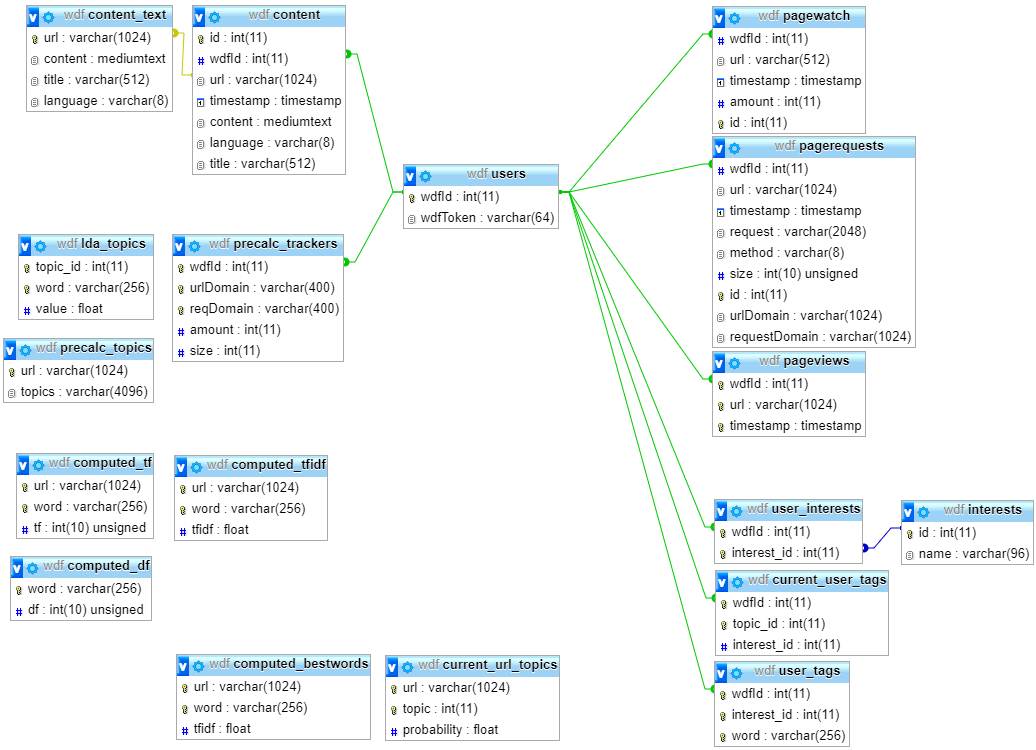
\includegraphics[height=0.8\textwidth]{images/design/db}
			\caption{Schéma des tables de la base de données}
			\label{db}
		\end{figure}

		Toutes les informations sont centralisées dans une base de données MySQL. La figure~\ref{db} montre le schéma global des tables de la base de données. L'utilisation de chaque table est décrite dans la section suivante, lors de leur accès. La section suivante décrit chacun des champs des tables de la base de données.

		\subsubsection{Table \texttt{content}}\label{table-content}
			La table \texttt{content} sert à stocker le contenu HTML initial des pages téléchargées. Il s'agit du contenu \glsdisp{DOM}{DOM} de la page après la fin du chargement et de l'exécution du JavaScript présent sur celle-ci.

			\begin{tabular}{rl}
				\textbf{Colonne} & \textbf{Description} \\
				\hline
				\texttt{id}       & Clé primaire artificielle \\
				\texttt{wdfId}    & Identifiant de l'utilisateur ayant accédé à la page \\
				\texttt{url}      & URL de la page \\
				\texttt{timestamp} & Date du téléchargement \\
				\texttt{content}  & Contenu \glsdisp{DOM}{DOM} entier \\
				\texttt{language} & Langue détectée du texte \\
				\texttt{title}    & Contenu de la balise \texttt{\small{title}} \\
			\end{tabular}
		
		\subsubsection{Table \texttt{content\_text}}\label{table-content-text}
			La table \texttt{content\_text} sert à stocker le contenu textuel des pages après le traitement décrit au paragraphe \ref{d-recolte}.

			\begin{tabular}{rl}
				\textbf{Colonne} & \textbf{Description} \\
				\hline
			    \texttt{url}      & URL de la page \\
				\texttt{content}  & Contenu textuel lemmatisé \\
				\texttt{title}    & Contenu de la balise \texttt{\small{title}} \\
				\texttt{language} & Langue détectée du texte \\
			\end{tabular}
		
		\subsubsection{Table \texttt{users}}\label{table-users}
			La table \texttt{users} sert à stocker les utilisateurs enregistrés sur l'extension.

			\begin{tabular}{rl}
				\textbf{Colonne} & \textbf{Description} \\
				\hline
			    \texttt{wdfId}    & Numéro d'identifiant \\
				\texttt{wdfToken} & Token du client \\
			\end{tabular}
		
		\subsubsection{Table \texttt{pagewatch}}\label{table-pagewatch}
			La table \texttt{pagewatch} sert à enregistrer le temps passé par les utilisateurs sur les différentes pages web qu'ils visitent.

			\begin{tabular}{rl}
				\textbf{Colonne} & \textbf{Description} \\
				\hline
			    \texttt{wdfId}    & Numéro d'identifiant \\
				\texttt{url}  & URL de la page \\
				\texttt{timestamp} & Date de visualisation \\
				\texttt{amount} & Temps regardé [sec] \\
				\texttt{id} & Clé primaire artificielle \\
			\end{tabular}
		
		\subsubsection{Table \texttt{pagerequests}}\label{table-pagerequests}
			La table \texttt{pagerequests} sert à enregistrer les requêtes envoyées par le navigateur des utilisateurs.

			\begin{tabular}{rl}
				\textbf{Colonne} & \textbf{Description} \\
				\hline
			    \texttt{wdfId}    & Numéro d'identifiant \\
				\texttt{url}  & URL de la page \\
				\texttt{timestamp} & Date de visualisation \\
				\texttt{request} & URL requêtée \\
				\texttt{method} & Méthode HTTP \\
				\texttt{size} & Taille de la requête \\
				\texttt{id} & Clé primaire artificielle \\
				\texttt{urlDomain} & Domaine de l'URL actuelle \\
				\texttt{requestDomain} & Domaine de l'URL requêtée\\
			\end{tabular}
		
		\subsubsection{Table \texttt{pageviews}}\label{table-pageviews}
			La table \texttt{pageviews} sert à enregistrer les ouvertures d'URL de la part des utilisateurs.

			\begin{tabular}{rl}
				\textbf{Colonne} & \textbf{Description} \\
				\hline
			    \texttt{wdfId} & Numéro d'identifiant \\
				\texttt{url}   & URL de la page \\
				\texttt{timestamp} & Date de visualisation \\
			\end{tabular}
		
		\subsubsection{Table \texttt{user\_interests}}\label{table-user-interests}
			La table \texttt{user\_interests} sert à enregistrer les centres d'intérêt que les utilisateurs déclarent.

			\begin{tabular}{rl}
				\textbf{Colonne} & \textbf{Description} \\
				\hline
			    \texttt{wdfId} & Numéro d'identifiant \\
				\texttt{interest\_id} & Numéro d'intérêt \\
			\end{tabular}
		
		\subsubsection{Table \texttt{interests}}\label{table-interests}
			La table \texttt{interests} sert à enregistrer la liste de centres d'intérêt que les utilisateurs peuvent choisir.

			\begin{tabular}{rl}
				\textbf{Colonne} & \textbf{Description} \\
				\hline
			    \texttt{id} & Numéro d'intérêt \\
				\texttt{name} & Nom de l'intérêt \\
			\end{tabular}
		
		\subsubsection{Table \texttt{current\_user\_tags}}\label{table-current-user-tags}
			La table \texttt{current\_user\_tags} sert à enregistrer les associations que les utilisateurs ont crée entre un topic LDA actuel et un centre d'intérêt renseigné.

			\begin{tabular}{rl}
				\textbf{Colonne} & \textbf{Description} \\
				\hline
				\texttt{wdfId} & Numéro d'identifiant \\
			    \texttt{topic\_id} & Numéro du topic \\
				\texttt{interest\_id} & Numéro de l'intérêt \\
			\end{tabular}
		
		\subsubsection{Table \texttt{user\_tags}}\label{table-user-tags}
			La table \texttt{user\_tags} sert à enregistrer les associations que les utilisateurs ont crée entre un \textbf{précédent} topic LDA représenté par quelques mots et un centre d'intérêt.

			\begin{tabular}{rl}
				\textbf{Colonne} & \textbf{Description} \\
				\hline
				\texttt{wdfId} & Numéro d'identifiant \\
			    \texttt{topic\_id} & Numéro du topic \\
				\texttt{words} & Trois mots du topic \\
			\end{tabular}
		
		\subsubsection{Table \texttt{precalc\_trackers}}\label{table-precalc-trackers}
			La table \texttt{precalc\_trackers} sert à enregistrer les informations pré-calculées concernant le nombre de requêtes entre les domaines visités par l'utilisateur.

			\begin{tabular}{rl}
				\textbf{Colonne} & \textbf{Description} \\
				\hline
				\texttt{wdfId} & Numéro d'identifiant \\
			    \texttt{urlDomain} & Domaine de l'URL actuelle \\
				\texttt{requestDomain} & Domaine de l'URL requêtée \\
				\texttt{amount} & Nombre de requêtes \\
				\texttt{size} & Taille totale des requêtes \\
			\end{tabular}
		
		\subsubsection{Table \texttt{precalc\_topics}}\label{table-precalc-topics}
			La table \texttt{precalc\_topics} sert à enregistrer les informations pré-calculées sur les topics relatifs à chaque page web.

			\begin{tabular}{rl}
				\textbf{Colonne} & \textbf{Description} \\
				\hline
				\texttt{url} & URL de la page \\
			    \texttt{topics} & JSON des topics associés \\
			\end{tabular}
		
		\subsubsection{Table \texttt{lda\_topics}}\label{table-lda-topics}
			La table \texttt{lda\_topics} sert à enregistrer les informations des topics LDA du modèle actuel.

			\begin{tabular}{rl}
				\textbf{Colonne} & \textbf{Description} \\
				\hline
				\texttt{topic\_id} & Numéro du topic \\
			    \texttt{topics} & Mot associé \\
			    \texttt{value} & Probabilité du mot \\
			\end{tabular}
		
		\subsubsection{Table \texttt{computed\_tf}}\label{table-computed-tf}
			La table \texttt{computed\_tf} sert à enregistrer la valeur TF de chaque mot dans chaque page web. Cette table est uniquement là dans un but d'archivage, et n'est pas lue directement.

			\begin{tabular}{rl}
				\textbf{Colonne} & \textbf{Description} \\
				\hline
				\texttt{url} & URL de la page \\
			    \texttt{word} & Mot \\
			    \texttt{tf} & Term Frequency selon TF-IDF \\
			\end{tabular}
		
		\subsubsection{Table \texttt{computed\_df}}\label{table-computed-df}
			La table \texttt{computed\_df} sert à enregistrer la valeur DF de chaque mot dans chaque page web. Cette table est uniquement là dans un but d'archivage, et n'est pas lue directement.

			\begin{tabular}{rl}
				\textbf{Colonne} & \textbf{Description} \\
				\hline
			    \texttt{word} & Mot \\
			    \texttt{df} & Document Frequency selon TF-IDF \\
			\end{tabular}
		
 		\subsubsection{Table \texttt{computed\_tfidf}}\label{table-computed-tfidf}
			La table \texttt{computed\_tfidf} sert à enregistrer la valeur TF-IDF de chaque mot dans chaque page web.

			\begin{tabular}{rl}
				\textbf{Colonne} & \textbf{Description} \\
				\hline
				\texttt{url} & URL de la page \\
			    \texttt{word} & Mot \\
			    \texttt{df} & Score final TF-IDF \\
			\end{tabular}
		
		\subsubsection{Table \texttt{computed\_bestwords}}\label{table-computed-bestwords}
			La table \texttt{computed\_bestwords} sert à enregistrer les meilleurs mots selon TF-IDF de chaque page web.

			\begin{tabular}{rl}
				\textbf{Colonne} & \textbf{Description} \\
				\hline
				\texttt{url} & URL de la page \\
			    \texttt{word} & Mot \\
			    \texttt{tfidf} & Score final TF-IDF \\
			\end{tabular}
		
		\subsubsection{Table \texttt{current\_url\_topics}}\label{table-current-url-topics}
			La table \texttt{current\_url\_topics} sert à enregistrer les meilleurs topics du modèle LDA actuel pour chaque page web.

			\begin{tabular}{rl}
				\textbf{Colonne} & \textbf{Description} \\
				\hline
				\texttt{url} & URL de la page \\
			    \texttt{topic} & Numéro du topic \\
			    \texttt{probability} & Probabilité du topic pour la page \\
			\end{tabular}
		

	\FloatBarrier

	\subsection{Interface}

		L'interface a connu de nombreuses versions au fur et à mesure du projet. Cependant, le thème et le but commun de ces pages n'a pas changé : Montrer à l'utilisateur les informations qu'il révèle, ainsi que des possibles utilisations de celles-ci. Le design initial des visualisation était très visuel et varié et a progressé vers des pages plus utilitaires.

		L'interface se divise en trois onglets distincts, chacun tentant de représenter une partie des informations : Settings, Profil, et Trackers.

		\subsubsection{Settings}

			La page Settings laisse la possibilité à l'utilisateur de renseigner ces centres d'intérêt en les sélectionnant parmi une liste d'une centaine d'entre-eux. Cette centaine d'intérêts sont ceux que Google utilise pour "classifier" les visiteurs de sites web utilisant Google Analytics, nous estimons donc que ces intérêts font sens. 

		\subsubsection{Profil}

			\begin{figure}[!h]
				\centering
				\includegraphics[width=0.8\textwidth]{images/design/mockup_profile}
				\caption{Maquette de la page de Profil}
				\label{d-mockup-profile}
			\end{figure}

			La page Profil cherche à montrer le résultat de l'analyse des pages visitées par l'utilisateur, tentant de retrouver et de lui montrer quels sont ses centres d'intérêts. La figure~\ref{d-mockup-profile} montre les différentes vues prévues initialement :

			\begin{description}
				\item[1 Word Cloud] Cette vue cherche à mettre rapidement en valeur les mots les plus consultés par l'utilisateur en affichant un nuage de mots, où les plus grand seraient les plus vus. 
				\item[2 Interests graph] Cette visualisation cherche à rassembler les mots fréquemment lus par l'utilisateur en topics, eux-même liés entre eux. Le but est de montrer une synthèse du Word Cloud.
				\item[3 Website themes] Cette partie cherchait à montrer les mots redondants ainsi que les thèmes trouvés sur certains sites web.
				\item[4 Most visited sites] Ce graphique en barres cherche à montrer à l'utilisateur quels sont les sites qu'il a le plus souvent visité, c'est-à-dire ouverts l'URL, peu importe le temps passé sur chaque site.
				\item[5 Most watched sites] Ce graphique, contrairement au 4, cherche à montrer à l'utilisateur le temps total passé à regarder chaque page.
				\item[6 History of websites] Ce graphique cherche à montrer à l'utilisateur la fluctuation de sa visite de sites web sur la durée.
				\item[7 History of interests] Ce graphique cherche à mettre en lumière les sujets les plus visités par l'utilisateur sur une période de temps afin de potentiellement détecter des tendances ou des changements dans son comportement.
			\end{description}

		\FloatBarrier

		\subsubsection{Trackers}

			La page Trackers montre la liste des différents trackers contactés au cours de la navigation, ainsi que les domaines les ayant contactés.

			Les requêtes effectuées depuis une page vers le même domaine ne sont pas comptées car on estime qu'il s'agit de trafic que l'on sait qui va prendre place, peu importe la page contactée : Il est évident qu'elle va chercher à charger du contenu provenant du même domaine.
			
			La figure~\ref{d-mockup-trackers1} montre les 4 premières visualisations conceptualisées de la page Trackers, et la figure~\ref{d-mockup-trackers2} montre les 4 dernières.

			\begin{figure}[!h]
				\centering
				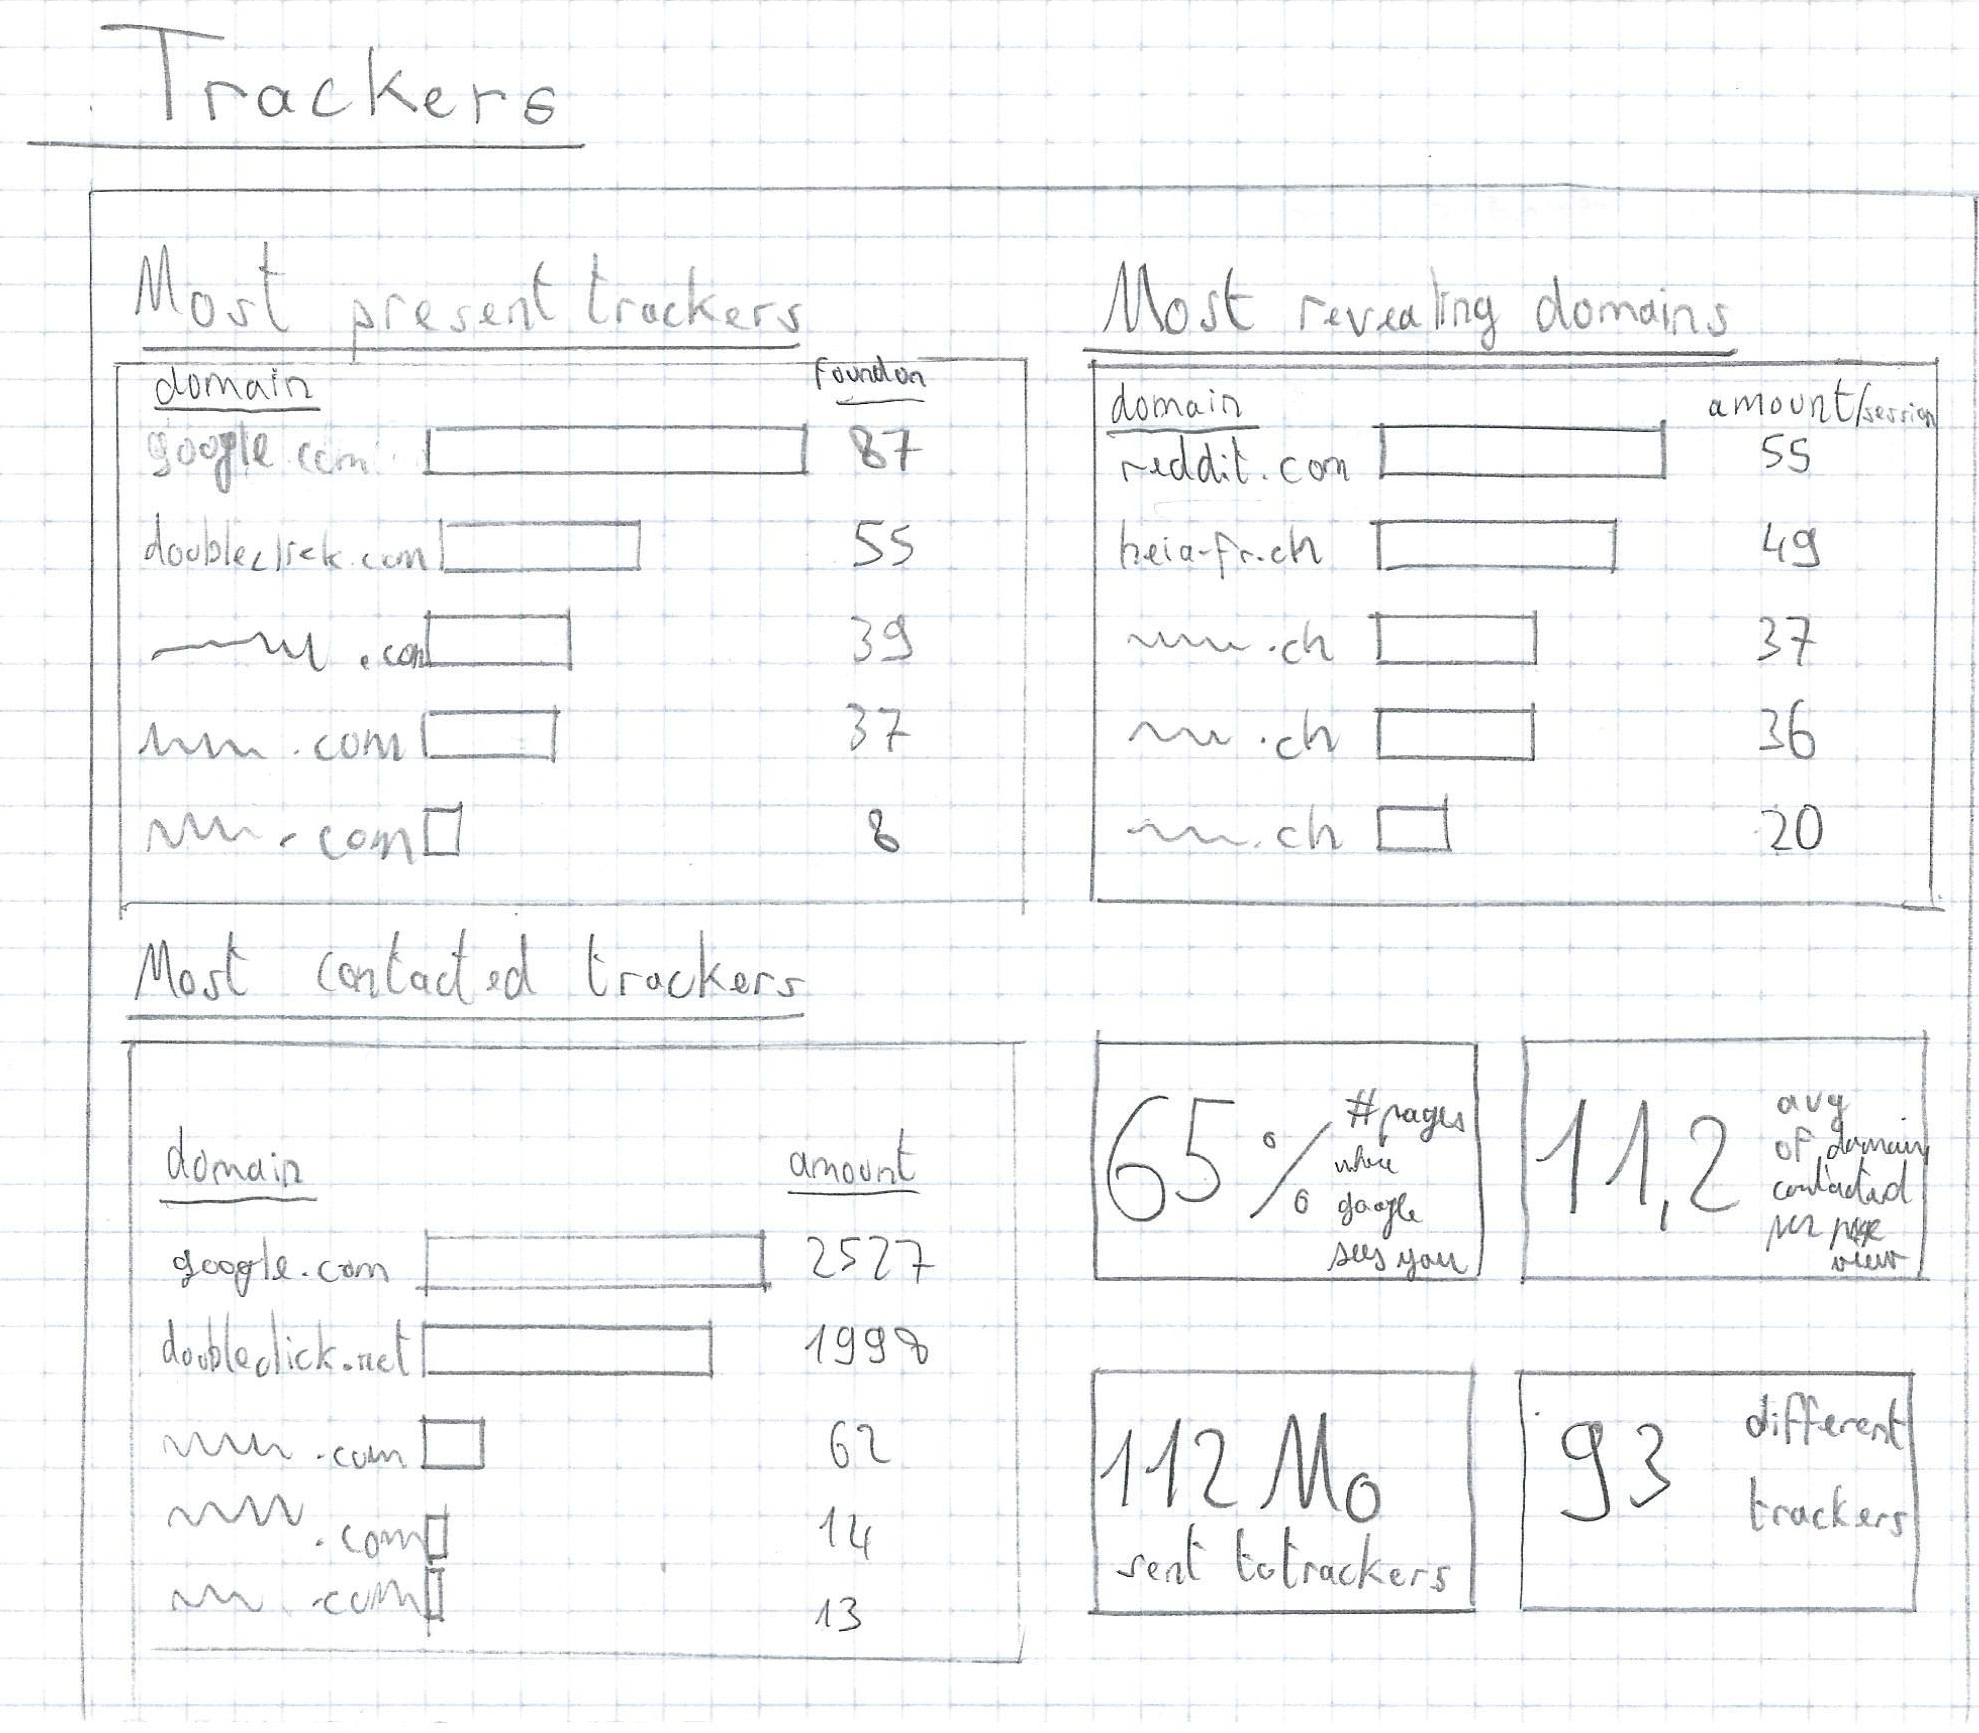
\includegraphics[width=0.8\textwidth]{images/design/mockup_trackers1}
				\caption{Maquette de la page de Trackers}
				\label{d-mockup-trackers1}
			\end{figure}

			\begin{description}
				\item[8 Most present trackers] Ce graphique en barres montrait les trackers potentiels contactés depuis  le plus grand nombre de pages différentes.
				\item[9 Most revealing trackers] Ce graphique en barres montrait une moyenne par domaine du nombre de requêtes effectuées vers des trackers potentiels.
				\item[10 Most contacted trackers] Ce graphique en barres montrait les potentiels trackers les plus contactés au total, depuis n'importe quelle page.
				\item[11 Stats] Quelques nombres montrent des statistiques générales de l'utilisateur afin de lui faire prendre compte de certaines mesures. Par exemple, la taille totale d'informations envoyées aux trackers potentiels, ou le nombre de ceux-ci contactés.
			\end{description}

			\FloatBarrier

			\begin{figure}[!h]
				\centering
				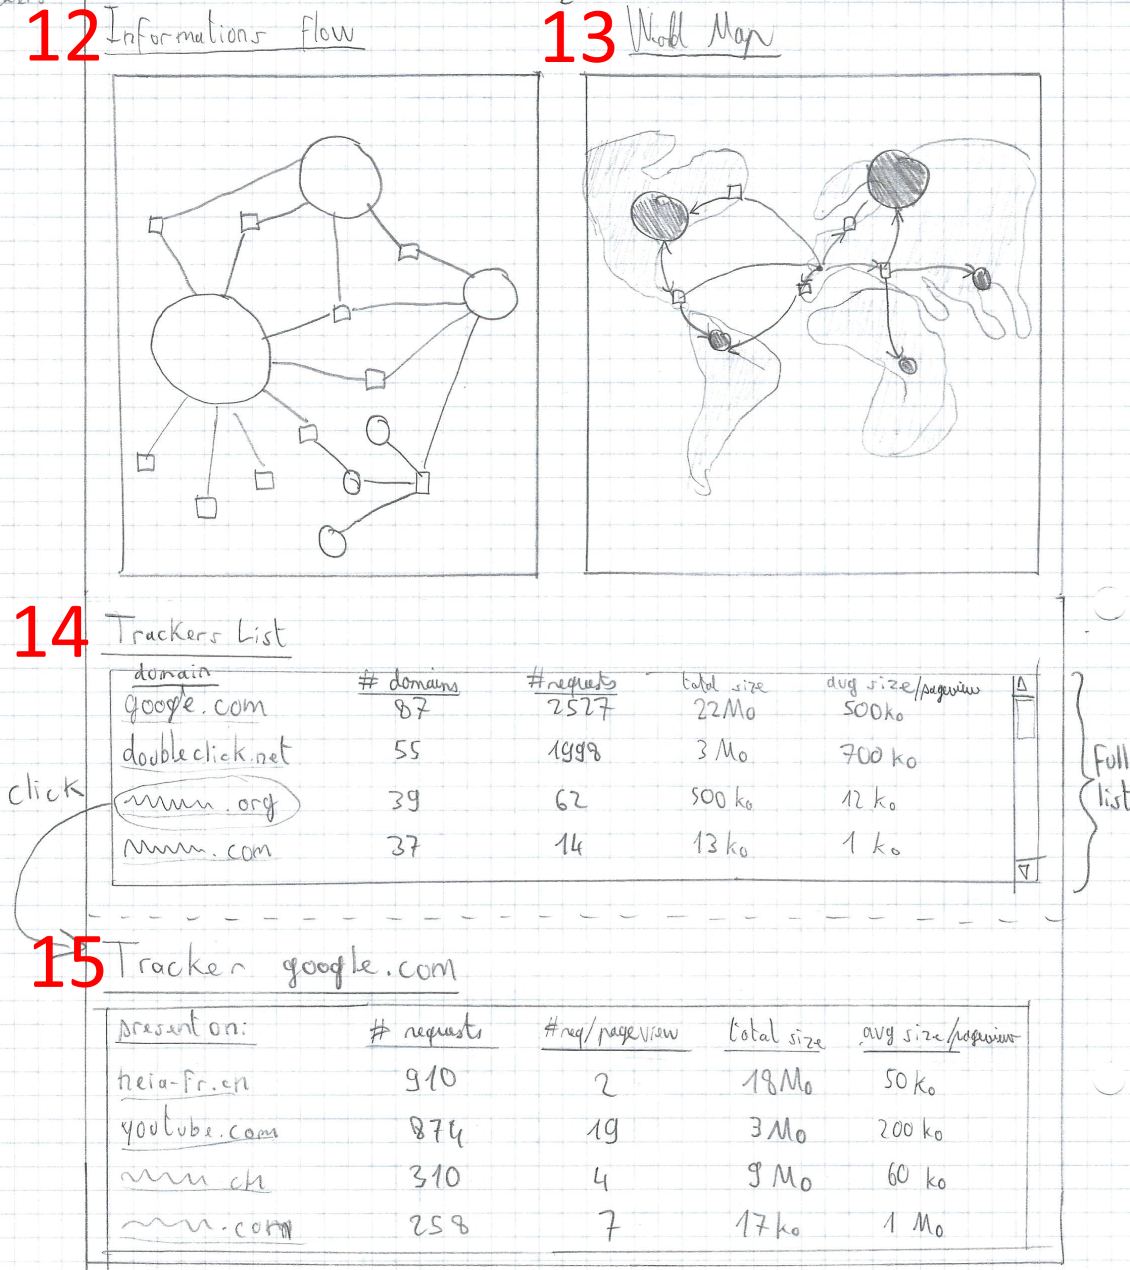
\includegraphics[width=0.8\textwidth]{images/design/mockup_trackers2}
				\caption{Suite de la maquette de la page de Trackers}
				\label{d-mockup-trackers2}
			\end{figure}

			\begin{description}
				\item[12 Informations flow] Cette visualisation sous forme de graphe cherche à montrer quels sont les domaines les plus connectés entre eux. Le but est de rassembler des domaines et sous-domaines afin de montrer lesquels de ceux-ci communiquent le plus.
				\item[13 World map] Cette visualisation est très semblable à la précédente. Les domaines sont à présent placés sur leur emplacement géographique afin de se rendre compte du trafic réel physique engendré par ces requêtes.
				\item[14 Trackers list] Cette partie montre de manière exhaustive l'ensemble des requêtes effectuées vers un domaine. Le but est de permettre aux utilisateurs curieux de parcourir l'ensemble des données de manière plus fine. Un clic sur un tracker ouvre la vue 15.
				\item[15 Selected tracker] Ce tableau s'ouvre en sélectionnant un tracker potentiel de la vue 14. Il montre l'ensemble des domaines ayant contacté le potentiel tracker sélectionné.
			\end{description}

			\paragraph{Topics graph}

				Le "topics graph" cherche à rassembler les mots en thèmes, et monte d'une manière plus synthétique les thèmes estimés que l'utilisateur parcourt fréquemment. À chaque thème est lié un ou plusieurs mots, qui représentent le thème d'une manière générale. Chaque cercle du graphe représente soit un thème, soit un mot.

				Le but de cette visualisation est de montrer que nous pouvons déduire des thèmes et ainsi montrer un traitement plus fin des intérêts de l'utilisateur, que simplement additionner une liste de mots. Dans le marketing, les thèmes découverts pourraient être utilisés pour labelliser les utilisateurs à qui faire apparaître une publicité.
\chapter{Implémentation}
%%%%%%%%%%%%%%%%%%%%%%%%%%
%                          %
% ----- INTRODUCTION ----- %
%                          %
%%%%%%%%%%%%%%%%%%%%%%%%%%

\section{Technologies}

	\subsection{Introduction}

		Dans cette section se trouveront des schémas représentant des algorithmes. Les étapes de ceux-ci peuvent être exécutés à trois moments différents, indiqué sur leurs schémas :
		\begin{description}
			\item[Offline] Les étapes effectuées "offline" recquièrent une intervention de l'administrateur. C'est à lui de décider quand ces traitements doivent intervenir car ils ne peuvent pas être effectuées pendant que le serveur fonctionne.
			\item[Serveur] Les étapes effectuées sur le "serveur" sont calculées pendant que le serveur est en ligne, typiquement lorsque celui-ci reçoit une requête.
			\item[Client] Les étapes s'effectuant sur le "client" sont calculées dans le navigateur de l'utilisateur actuel.
		\end{description}

	\subsection{Offline}

		Certains scripts doivent être lancées ponctuellement par l'administrateur afin d'exécuter des opérations coûteuses de calcul. Le lancement de ces opérations peut se faire manuellement, ou leur lancement peut être programmé à l'aide d'un script d'automatisation.

		Chaque opération est lancée à l'aide d'un script Python3.6 indépendant, se trouvant dans un dossier nommé \texttt{/script}. Ceux-ci nécessitent généralement d'accéder à la base de données pour effectuer des opérations, il est donc nécessaire de leur fournir les identifiants de connexion à la base de données, ou de les laisser puiser dans le script de configuration à la racine du projet. 

	\subsection{Serveur}

		Le serveur est développé en Python3.6, et utilise le framework Flask. Flask permet de définir rapidement le comportement d'un serveur web basique en mappant des fonctions à des endpoints de l'API.

		Par exemple, à l'aide d'une combinaison de décorateurs fournis par Flask et crées par nous-même, nous pouvons très facilement spécifier le comportement d'une méthode. La figure~\ref{i-code-server} montre le peu de code nécessaire pour définir l'endpoint de vérification de la connexion de l'utilisateur.

		\begin{figure}[!h]
			\centering
			\begin{lstlisting}[language=python]
@app.route("/api/connectionState", methods=['GET'])
@userConnected
@apiMethod
def connectionState(wdfId):
    return jsonify({'success': "Connected", "wdfId": wdfId})\end{lstlisting}
			\caption{Code de la méthode de vérification de connexion}
			\label{i-code-server}
		\end{figure}

		Naturellement, la plupart des autres méthodes nécessitent un accès à la base de données MySQL et donc du code plus conséquent.

		Ici, Flask n'écoute pas directement sur les ports concernés. Le programme entier est accessible derrière un serveur Apache pour des questions de sécurité : la communication entre l'extension, l'interface et le serveur se fait en HTTPS, grâce à la gestion de SSL par Apache, et un certificat obtenu à l'aide de Let's Encrypt.


	\subsection{Client}

		\begin{wrapfigure}{r}{3cm}
			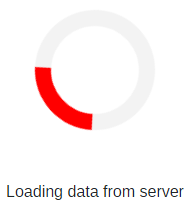
\includegraphics[width=2.9cm]{images/design/loading_spinner}
			\caption{Chargement des données}\label{i-loading}
		\end{wrapfigure} 

		L'interface est développée en JavaScript et TypeScript en utilisant le framework Vue.js. Comme plusieurs de ses autres équivalents, Vue.js permet d'organiser le code en composants réutilisables. Le but étant de développer une one-page app pour des raisons de réactivité de l'interface. Un des avantages de ce type de framework est donc la possibilité de configurer un router.

		Ceci permet à l'utilisateur d'avoir l'impression de naviguer entre plusieurs pages distinctes, alors que tout le processus prend place dans le framework lui-même, qui se charge de changer le contenu affiché sans nécessiter de requête supplémentaire au serveur.

		\begin{figure}[!h]
			\centering
			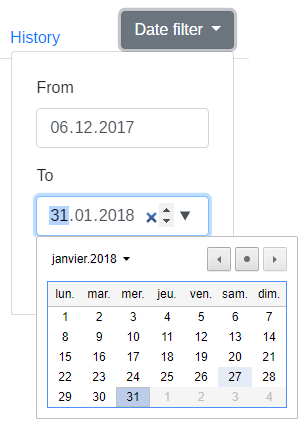
\includegraphics[width=7cm]{images/design/date_filter}
			\caption{Formulaire du filtre de dates}\label{i-filter}
		\end{figure}

		Au lancement de la page, l'interface entière est donc chargée sur le navigateur, et l'ensemble des données de l'utilisateur est demandée au serveur. La figure~\ref{i-loading} montre le spinner affiché à l'utilisateur pendant le chargement.

		Sur les pages de Profil, l'utilisateur a ensuite la possibilité de filtrer les données affichées par date. La figure~\ref{i-filter} montre le formulaire du filtre de données que l'utilisateur peut décider d'activer. Une fois activé après la sélection d'une date de début et d'une date de fin, la page entière se recharge en demandant au serveur le nouveau jeu de données correspondant aux dates entrées. Il s'agit d'un paramètre de recherche supplémentaire passé aux endpoints.

%
%
% WORDCLOUD
%
%

\section{Wordcloud}

	\subsection{Concept}
		Le wordcloud montre à l'utilisateur la liste des mots qu'il lit le plus fréquemment. Le visualisation est un amassage de mots de différentes tailles, placés d'une manière aléatoire sur un rectangle. Les mots les plus lus ont une taille plus grande afin d'attirer l'attention de l'utilisateur.

		Cette visualisation cherche à donner très rapidement une impression générale des thèmes que l'utilisateur parcourt lors de sa navigation.

		\begin{figure}[!h]
			\centering
			\subfloat[Maquette initiale de la vue]{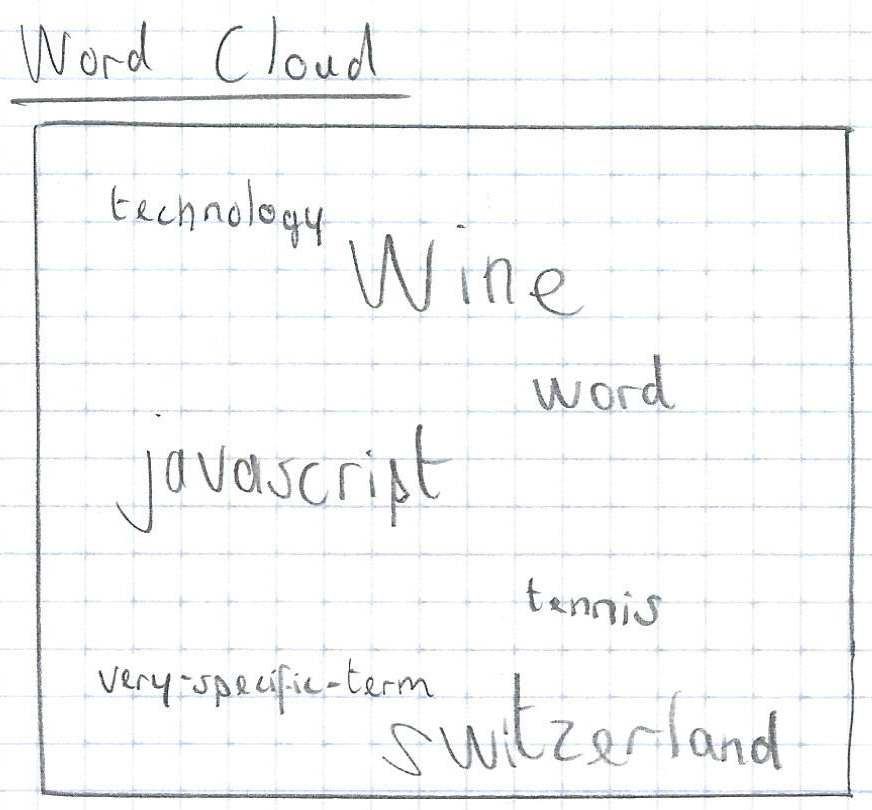
\includegraphics[width=0.33\textwidth,valign=t]{images/design/pages/wordcloud_mockup}}
			\subfloat[Exemple de résultat final]{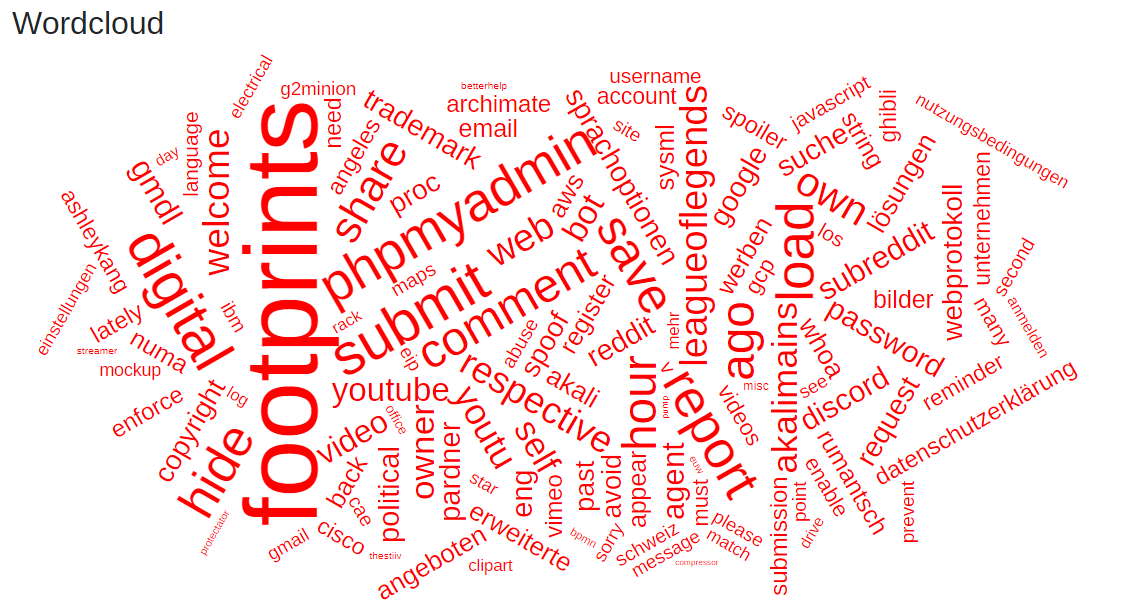
\includegraphics[width=0.66\textwidth,valign=t]{images/design/pages/wordcloud_final}}
			\caption{Maquette initiale et résultat final de la vue Wordcloud}
			\label{wordcloud_images}
		\end{figure}

		La figure~\ref{wordcloud_images} montre la différence entre la vue imaginée initialement et le résultat final.

	\subsection{Données}

		Les données source servant à constituer cette visualisation sont :
		\begin{description}
			\item[Temps de visualisation] : Temps de visualisation total de chaque page. Ces données sont stockées dans la table \texttt{pagewatch} (figure \ref{table-content}).
			\item[Poids TF-IDF] : Poids final selon l'algorithme TF-IDF de chaque mot. Ces données sont stockées dans la table \texttt{computed\_tfidf} (figure \ref{table-computed-tfidf}).
		\end{description}

	\subsection{Traitement}

		Afin de déterminer quels sont les mots affichés ainsi que leur taille sur la visualisation, on assigne un "poids" à chaque mot.

		La figure~\ref{wordcloud_algo} illustre le fonctionnement de l'algorithme utilisé :
		\begin{description}
			\item[A] On calcule le poids de chaque mot dans chaque document en effectuant la méthode de TF-IDF. Le poids TF-IDF de chaque mot est stocké dans la base de données, mais n'est pas constamment rafraîchi. L'opération de calcul des poids TF-IDF est une opération ponctuelle qui doit être lancée sur l'entièreté de la base de données par l'administrateur. Cette opération ne nécessite cependant pas de redémarrage du serveur.

			\item[B] On effectue la somme du temps que l'utilisateur a passé à regarder chaque page visitée. Cette opération est effectuée sur le serveur et est calculée en direct par une commande MySQL, elle est donc constamment à jour. L'interface obtient ce résultat en appelant l'endpoint \texttt{/api/mostWatchedSites} du serveur. Le résultat de cet appel est une liste de l'ensemble des pages web visitées, comprenant entre autres pour chaque page : 
			\begin{itemize}
				\item Son URL
				\item Le temps total de visite, en secondes
				\item Une liste des mots les plus significatifs selon TF-IDF ainsi que leur poids TF-IDF (normalisé entre 0 et 1)
			\end{itemize}
			
			On initialise un dictionnaire qui va contenir le poids de chaque mot.

			\item[C] Pour chaque page web, on multiplie l'indice TF-IDF de chaque mot avec le temps de visualisation de la page. On additionne ce résultat au poids actuel du mot.
			
			Une fois tous les mots de toutes les pages web traités, nous sommes en possession d'un dictionnaire nous indiquant le poids final de chaque mot. Ce poids est donc égal à la somme de l'indice TF-IDF du mot sur chaque page multiplié par le temps de visite sur cette page.
			
			\item[D] On trie les mots par leur poids final, et on ne conserve que les 200 premiers. Il s'agira des 200 mots présents sur le wordcloud.
			
			Pour chacun des 200 mots, leur taille sur le Wordcloud est égale à leur poids final.
		\end{description}

		\begin{figure}[!h]
			\centering
			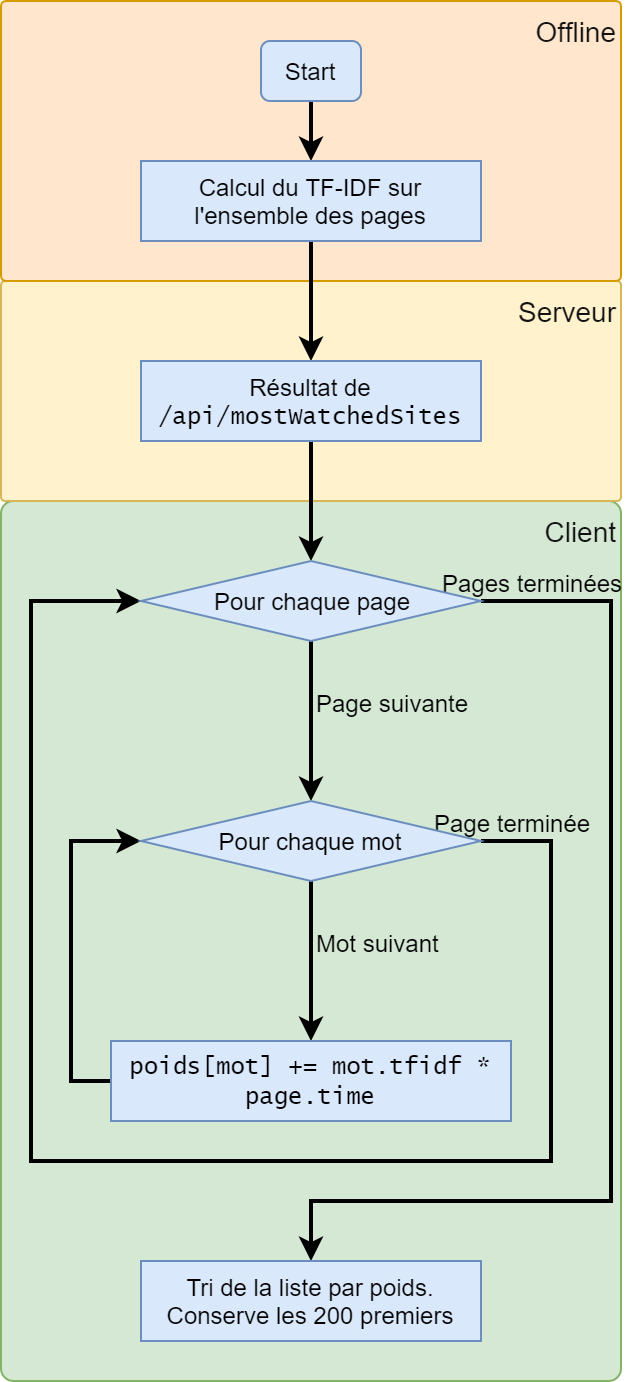
\includegraphics[height=1.15\textwidth]{images/design/pages/wordcloud_algo}
			\caption{Algorithme utilisé pour le Wordcloud}
			\label{wordcloud_algo}
		\end{figure}

	\subsection{Visualisation}

			La page va s'occuper d'agréger les résultats reçus du serveur. Ensuite, elle utilise les librairies \texttt{d3-cloud} ainsi que \texttt{d3} pour générer la visualisation du Wordcloud.

\clearpage

%
%
% TOPICS LIST
%
%

\section{Topics List}\label{topicslist}

	\subsection{Concept}

		Le "Topics List" cherche à rassembler les mots en thèmes, et montre d'une manière plus synthétique les thèmes estimés que l'utilisateur parcourt fréquamment. À chaque thème est lié un ou plusieurs mots, qui reprèsentent le thème d'une manière générale. Chaque cercle du graphe représente soit un thème, soit un mot.

		Le but de cette visualisation est de montrer que nous pouvons déduire des thèmes et ainsi montrer un traitement plus fin des intérêts de l'utilisateur, que simplement additionner une liste de mots. Dans le marketing, les thèmes découverts pourraient être utilisés pour labelliser les utilisateurs à qui faire apparaître une publicité.

		\begin{figure}[!h]
			\centering
			\subfloat[Maquette initiale de la vue]{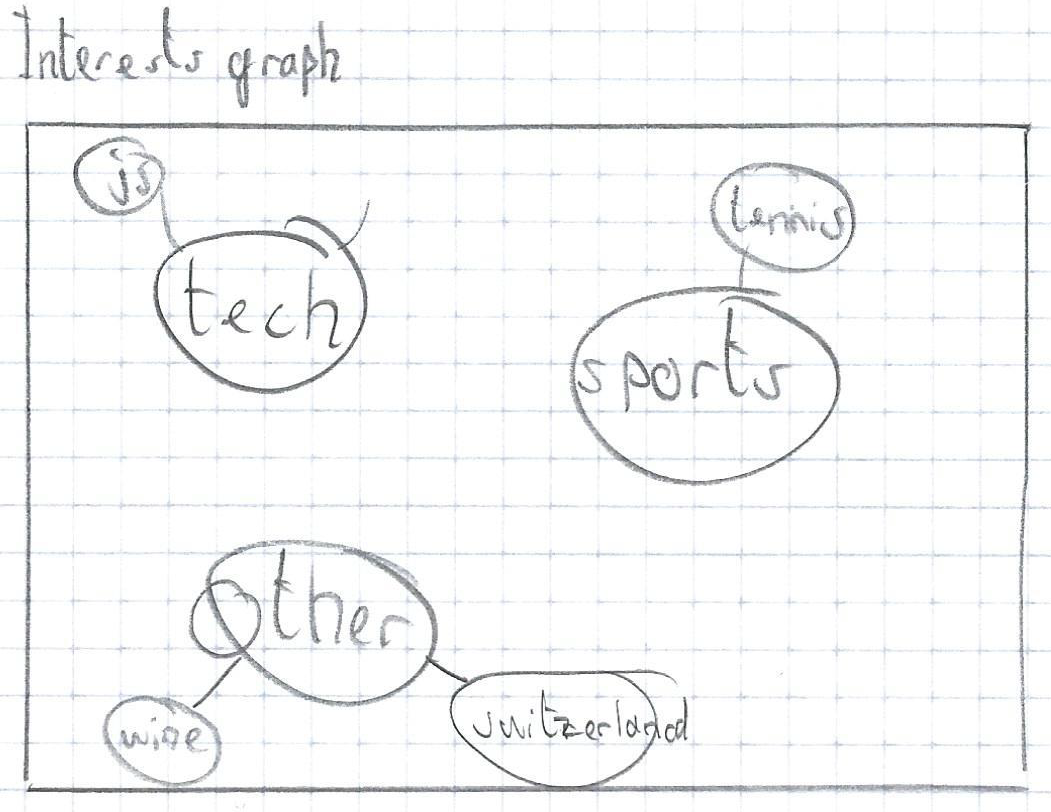
\includegraphics[width=0.33\textwidth,valign=t]{images/design/pages/topics_mockup}}
			\subfloat[Exemple de résultat final]{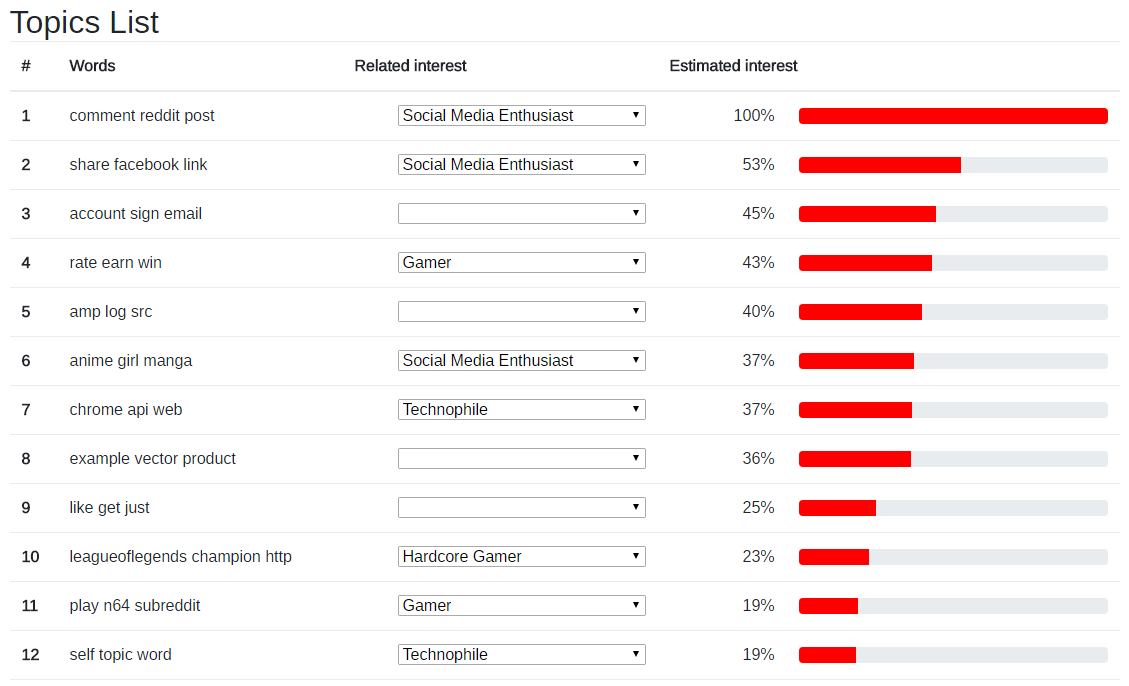
\includegraphics[width=0.66\textwidth,valign=t]{images/design/pages/topics_final}}
			\caption{Maquette initiale et résultat final de la vue Wordcloud}
			\label{topics_images}
		\end{figure}

		La figure~\ref{topics_images} montre la différence entre la vue imaginée et le résultat final. On note ici que le principe même de la vue ainsi que son nom sont différents qu'initialement.

	\subsection{Données}

		Les données source servant à constituer cette visualisation sont :
		\begin{description}
			\item[Temps de visualisation] : Temps de visualisation total de chaque page. Ces données sont stockées dans la table \texttt{pagewatch} (figure \ref{table-content}).
			\item[Topics LDA] : Liste des topics générés par le modèle LDA. Ces données sont stockées dans la table \texttt{lda\_topics} (figure \ref{table-lda-topics}).
			\item[Topics par page] : Liste pré-caluclée des topics trouvés pour chaque page. Ces données sont stockées dans la table \texttt{current\_url\_topics} (figure \ref{table-current-url-topics}).
			\item[Intérêts utilisateur] : Liste des intérêts renseignés par l'utilisateur. Ces données sont stockées dans la table \texttt{user\_interests} (figure \ref{table-user-interests}).
			\item[Correspondances topic-intrêt] : Liste des correspondances entre topic et intérêt renseignés par l'utilisateur. Ces données sont stockées dans la table \texttt{current\_user\_tags} (figure \ref{table-current-user-tags}).
		\end{description}

	\subsection{Traitement}

		Afin de déterminer quels sont les topics affichés ainsi que leur intérêt estimé, on assigne un "score" à chaque topic pour l'utilisateur.

		L'algorithme suivant, illustré par la figure~\ref{topics_algo}, est appliqué aux données sources :
		\begin{description}
			\item[A] On entraîne un modèle LDA avec un nombre défini de topics (typiquement 100) sur le contenu de l'ensemble des pages web, une page web représentant un document.

			Le modèle LDA est enregistré sur le disque local, et les résultats tirés de celui-ci, comme une la représentation en 5 mots de chaque topic, est maintenant stockés dans la base de données. Tout ceci n'est donc pas constamment rafraîchi. L'opération d'entraînement du modèle LDA est une opération ponctuelle qui doit être lancée sur l'entièreté de la base de données par l'administrateur. Cette opération nécessite le redémarrage du serveur, car de nombreuses mesures temporaires sont touchées.

			\item[B] Pour chaque page enregistrée, on demande au modèle LDA quels sont les 5 topics les plus probables avec leur score de probabilité. Ces informations sont également enregistrées dans la base de données. Jusqu'ici, toutes ces opérations sont donc déjà calculées et se font avant le lancement du serveur. Elles ne sont pas mises à jour en temps réel.
			
			\item[C] On effectue la somme du temps que l'utilisateur a passé à regarder chaque page visitée. Cette opération est effectuée sur le serveur et est calculée en direct par une commande MySQL, elle est donc constamment à jour. L'interface obtient ce résultat en appelant l'endpoint \texttt{/api/mostWatchedSites} du serveur. Le résultat de cet appel est une liste de l'ensemble des pages web visitées, comprenant entre autres pour chaque page : 
			\begin{itemize}
				\item Son URL
				\item Le temps total de visite, en secondes
				\item Une liste des topics les plus significatifs selon le modèle LDA ainsi que leur probabilité
			\end{itemize}

			\item[D] L'endpoint \texttt{/api/allTopics} renvoie la liste des topics générés par LDA ainsi que leur numéro d'identifiant.

			\item[E] L'endpoint \texttt{/api/getCurrentTags} renvoie la liste des associations que l'utilisateur a crée pour le modèle LDA courant. Il s'agit d'une liste de couples topicId $\longleftrightarrow$ interestId.

			\item[F] L'endpoint \texttt{/api/interestsList} renvoie la liste des 101 intérêts globaux à tous les utilisateurs.

			\item[G] On initialise un dictionnaire qui va contenir le score de chaque topic.
			
			Pour chaque page web, on multiplie la probabilité de chaque topic LDA avec le temps de visualisation de la page. On additionne ce résultat au score actuel du topic.
			
			Une fois tous les topics de toutes les pages web traités, nous sommes en possession d'un dictionnaire nous indiquant le score final de chaque topics. Ce score est donc égal à la somme de la probabilité du topic sur chaque page multiplié par le temps de visite sur cette page.
			
			\item[H] On trie les topics par leur score final, et on ne conserve que les 20 premiers. Il s'agira des 20 topics présents sur la page.

			\item[I] On sélectionne les centres d'intérêt de l'utilisateur, ainsi que les associations qu'il a déjà crée pour le modèle LDA actuel. On ajoute les associations aux topics de l'interface.
		\end{description}

		\begin{figure}[!h]
			\centering
			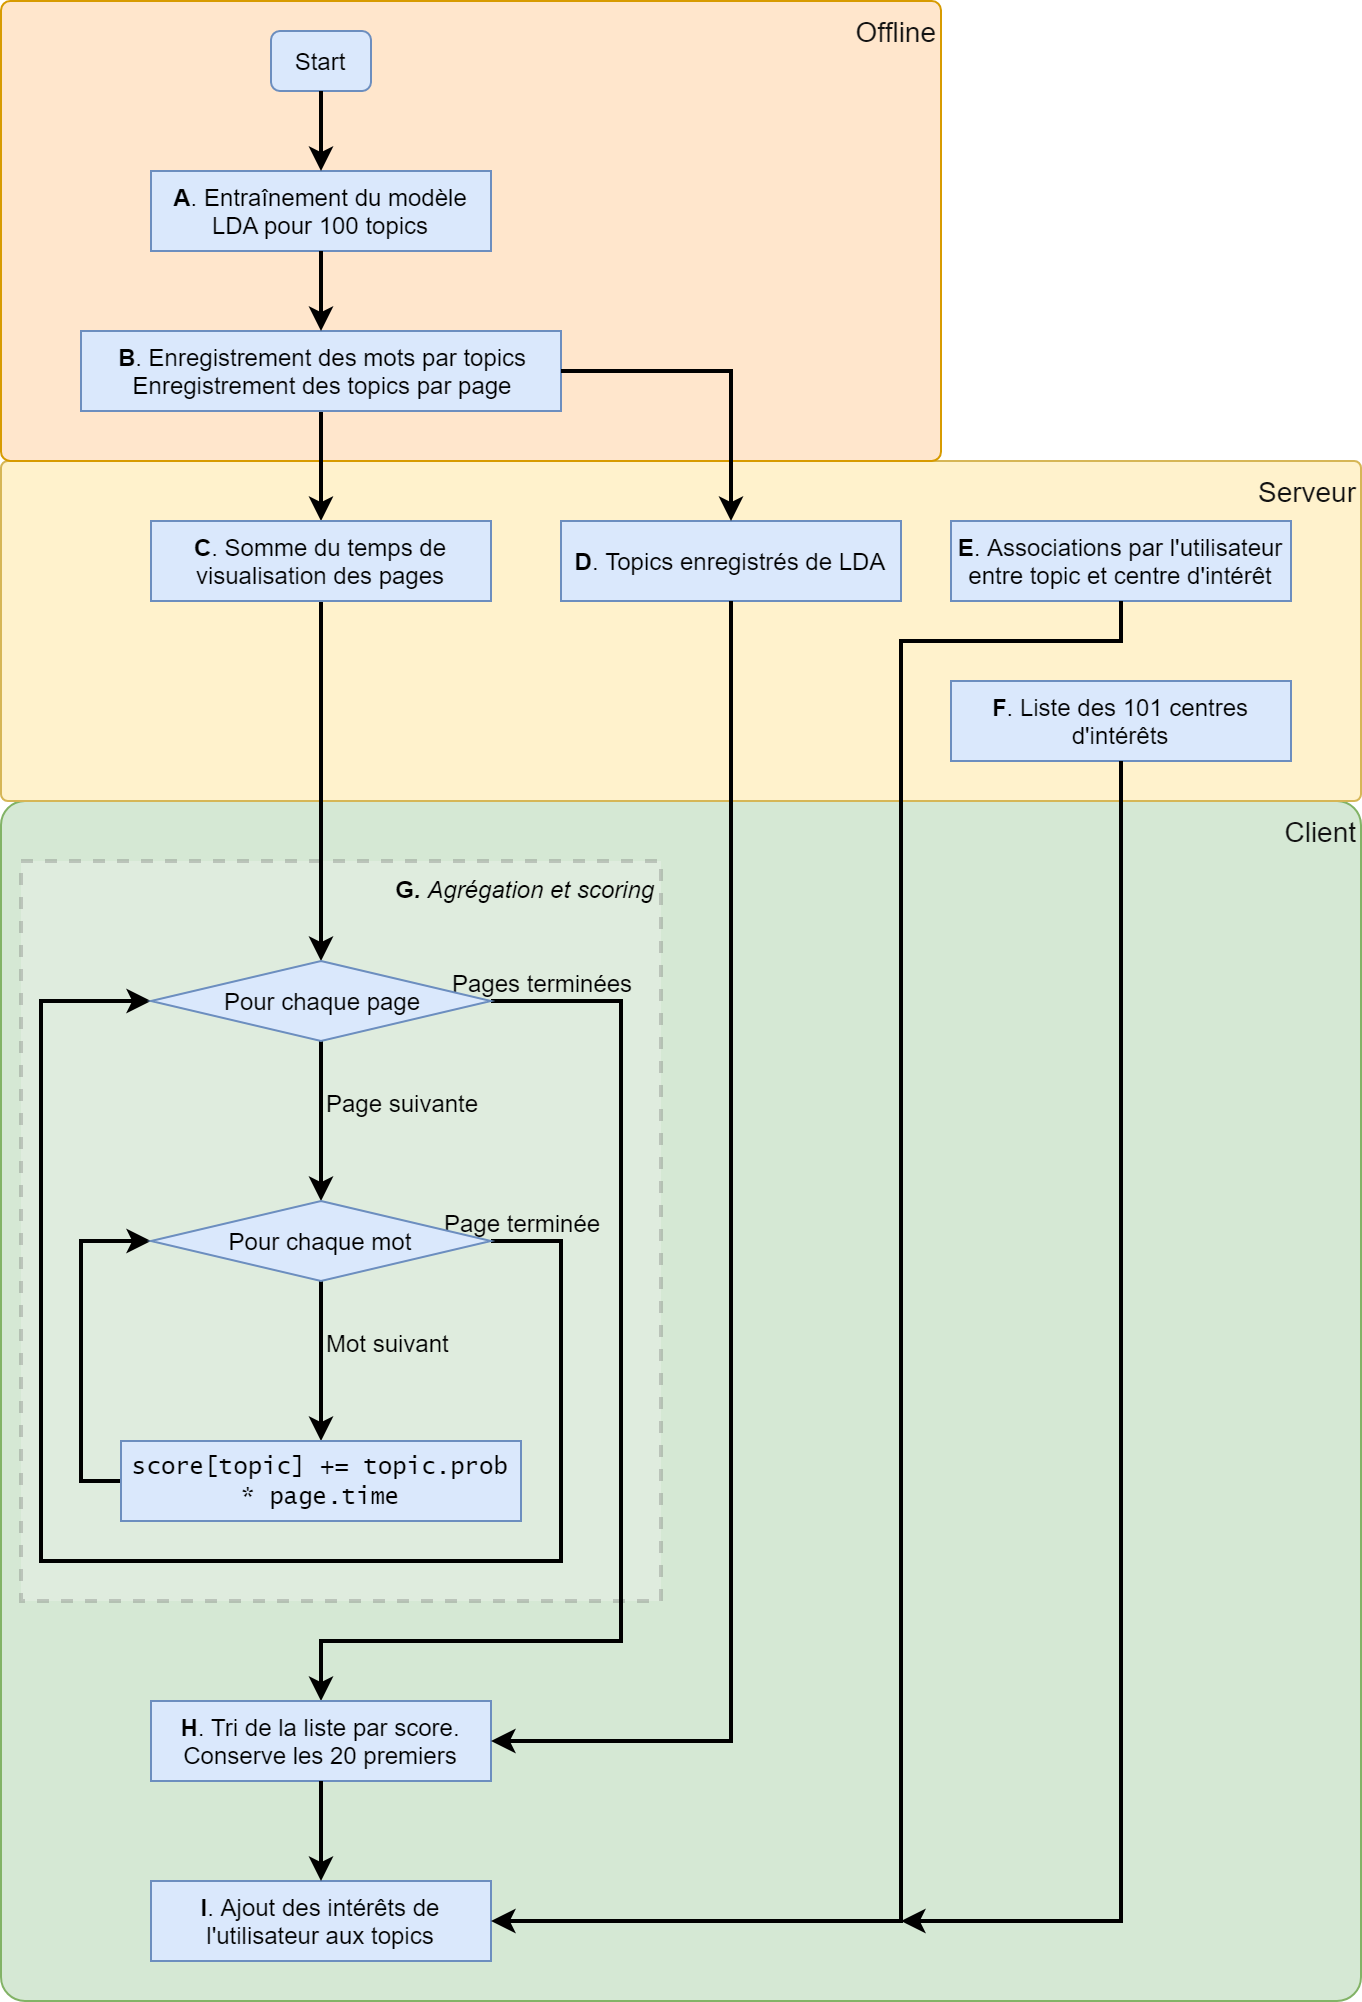
\includegraphics[height=1.35\textwidth]{images/design/pages/topics_algo}
			\caption{Algorithme utilisé pour le Topics List}
			\label{topics_algo}
		\end{figure}

	\subsection{Visualisation}

			La page va s'occuper d'agréger les résultats reçus du serveur. La liste est ensuite générée sous forme d'un tableau HTML en passant par un composant Vue personnalisé. Les barres d'intérêt sont des éléments \texttt{progressbar} venant de Bootstrap.

\clearpage

%
%
% MOST WATCHED
%
%

\section{Most Watched}

	\subsection{Concept}

		Les pages "Most Watched" et "Most Visited" montrent deux informations, mais sous une forme semblable. Ces pages affichent quelles pages web et les domaines que l'utilisateur a visité le plus. Plus précisément, "Most Watched" s'intéresse au temps réel passé à lire chaque page, et "Most Visited" s'intéresse au nombre d'ouvertures de l'URL.

		Le but est ici de faire prendre conscience à l'utilisateur qu'il est possible de se rendre compte de son activité une page web, et un grand nombre d'ouvertures d'un lien ne veut pas forcément dire un grand intérêt pour cette page.

		On profite également de cet espace pour afficher les mots relatifs aux pages web qui ont le plus d'intérêt, afin de montrer qu'il est possible de déterminer quels sont les mots importants d'une page web simplement en la comparant au contenu des autres pages.

		La figure~\ref{mostwatched_images} montre la différence entre la vue imaginée et le résultat final.

		\begin{figure}[!h]
			\centering
			\subfloat[Maquette initiale de la vue]{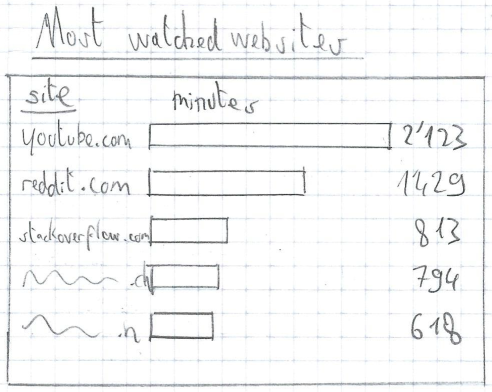
\includegraphics[width=0.33\textwidth,valign=t]{images/design/pages/mostwatched_mockup}}
			\subfloat[Exemple de résultat final]{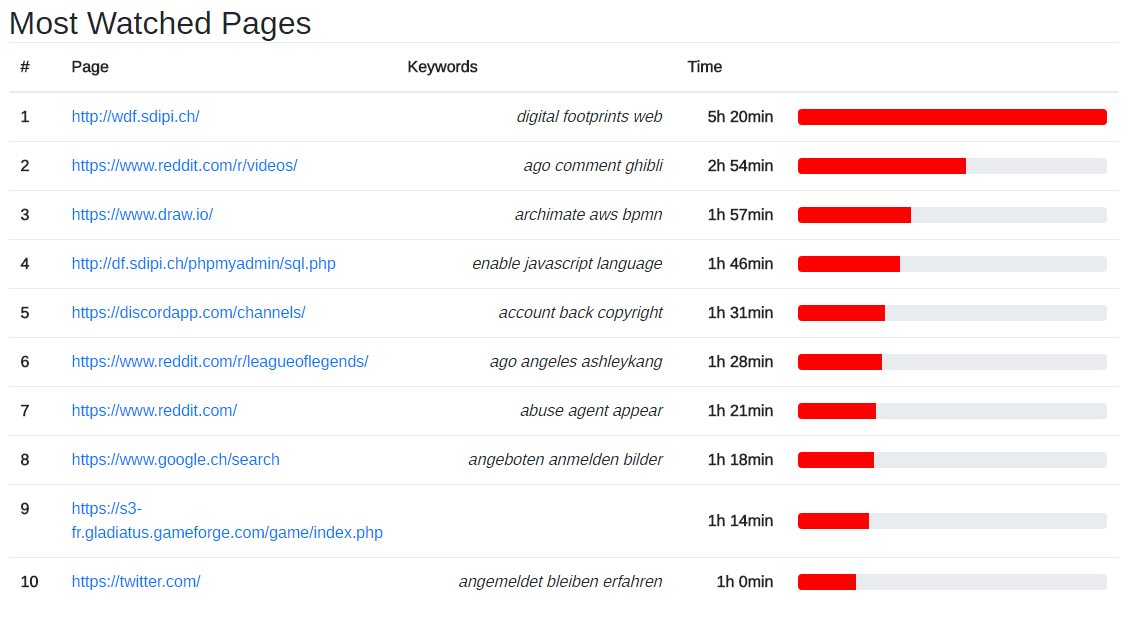
\includegraphics[width=0.66\textwidth,valign=t]{images/design/pages/mostwatched_final}}
			\caption{Maquette initiale et résultat final de la vue Most Watched}
			\label{mostwatched_images}
		\end{figure}

		Comme certaines pages web demandent une connexion pour être visualisées, par exemple la page d'accueil de \url{https://www.facebook.com}, nous omettons volontairement une liste de pages web dans ce classement, car nous n'avons pas d'informations intéressante sur leur contenu à montrer. En effet, nous ne téléchargeons volontairement pas de copie de la page vue par l'utilisateur pour des questions de protection de données privées. Notre serveur télécharge la version publique de l'URL visitée par l'utilisateur pour en déterminer son contenu. Ainsi, il ne fait pas sens d'analyser le contenu des pages générées dynamiquement par l'utilisateur.

	\subsection{Données}

		Les données source servant à constituer cette visualisation sont :
		\begin{description}
			\item[Temps de visualisation] : Temps de visualisation total de chaque page. Ces données sont stockées dans la table \texttt{pagewatch} (figure \ref{table-content}).
			\item[Nombre de visites] : Nombre total d'ouvertures de chaque URL. Ces données sont stockées dans la table \texttt{pageviews} (figure \ref{table-pageviews}).
			\item[Poids TF-IDF] : Poids final selon l'algorithme TF-IDF de chaque mot. Ces données sont stockées dans la table \texttt{computed\_tfidf} (figure \ref{table-computed-tfidf}).
		\end{description}

	\subsection{Traitement}

		Afin de déterminer quels sont les pages et les domaines affichés, on demande au serveur la liste triée des URLs les plus regardées et ouvertes.

		L'algorithme suivant, illustré par la figure~\ref{mostwatched_algo}, est appliqué aux données sources :
		\begin{description}
			\item[A] On calcule le poids de chaque mot dans chaque document en effectuant la méthode de TF-IDF. Le poids TF-IDF de chaque mot est stocké dans la base de données, mais n'est pas constamment rafraîchi. L'opération de calcul des poids TF-IDF est une opération ponctuelle qui doit être lancée sur l'entièreté de la base de données par l'administrateur. Cette opération ne nécessite cependant pas de redémarrage du serveur.

			\item[B] On effectue la somme du temps que l'utilisateur a passé à regarder chaque page visitée. Cette opération est effectuée sur le serveur et est calculée en direct par une commande MySQL, elle est donc constamment à jour. L'interface obtient ce résultat en appelant l'endpoint \texttt{/api/mostWatchedSites} du serveur. Le résultat de cet appel est une liste de l'ensemble des pages web regardées, comprenant entre autres pour chaque page : 
			\begin{itemize}
				\item Son URL
				\item Le temps total de visite, en secondes
				\item Une liste des mots les plus significatifs selon TF-IDF ainsi que leur poids TF-IDF (normalisé entre 0 et 1)
			\end{itemize}

			\item[C] On effectue la somme du nombre d'ouvertures de chaque page visitée. Cette opération est effectuée sur le serveur, et l'interface obtient ce résultat en appelant l'endpoint \texttt{/api/mostVisitedSites} du serveur. Le résultat de cet appel est une liste de l'ensemble des pages web visitées, comprenant entre autres pour chaque page : 
			\begin{itemize}
				\item Son URL
				\item Le nombre total d'ouvertures
				\item Une liste des mots les plus significatifs selon TF-IDF ainsi que leur poids TF-IDF (normalisé entre 0 et 1)
			\end{itemize}
			
			\item[D] Une fois la liste des pages les plus regardées obtenue, on ne conserve que les 10 premières d'entre-elles pour des raisons visuelles. Ces 10 premières pages sont alors affichées.

			\item[E] Ensuite, on cherche à agréger le temps de visualisation par domaine plutôt que par page, afin d'avoir une vue d'ensemble. On additionne donc le temps passé à regarder les pages d'un même domaine.

			\item[F] On trie la nouvelle liste de domaines crée par leur temps total de visualisation, et on ne garde également que les 10 premiers d'entre-eux pour les afficher.

			\item[G] On s'occupe ensuite du traitement du nombre d'ouvertures de chaque page. On ne conserve également que les 10 plus ouvertes d'entre-elles pour des raisons visuelles, elles sont alors affichées dans la liste.

			\item[H] Ensuite, on agrèger le nombre d'ouvertures par domaine plutôt que par page, afin d'avoir une vue d'ensemble. On additionne donc le temps passé à regarder les pages d'un même domaine.

			\item[I] On trie la nouvelle liste de domaines crée par leur temps total de visualisation, et on ne garde également que les 10 premiers d'entre-eux pour les afficher.
		\end{description}

		\begin{figure}[!h]
			\centering
			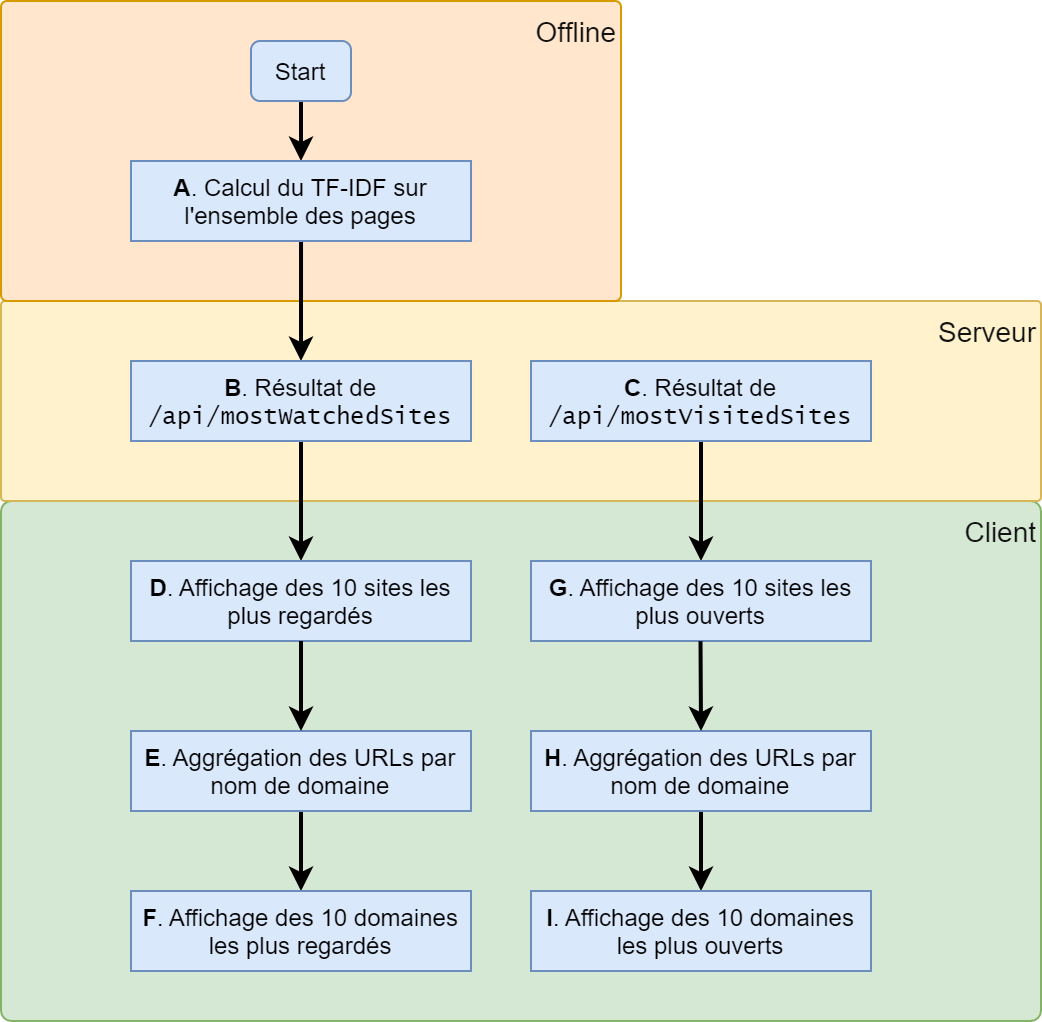
\includegraphics[height=0.8\textwidth]{images/design/pages/mostwatched_algo}
			\caption{Algorithme utilisé pour les pages "Most Watched" et "Most Visited"}
			\label{mostwatched_algo}
		\end{figure}

	\subsection{Visualisation}

		La page va s'occuper d'agréger les résultats reçus du serveur. Chaque liste est ensuite générée sous forme d'un tableau HTML en passant par un composant Vue personnalisé. Les barres relatives à la quantité exprimée par chaque tableau ajoute un élément de comparaison visuel, et sont des éléments \texttt{progressbar} venant de Bootstrap.

\clearpage

%
%
% HISTORY
%
%

\section{History}

	\subsection{Concept}

		La page "History" permet de montrer à l'utilisateur la variation de ses habitudes au cours du temps durant lequel il a utilisé l'extension. Deux graphiques sont présents sur cette page : Le premier montre la tendence à visiter des pages relatées à certains topics, et l'autre montre la tendence dans la visite de pages contenant certains mots particuliers. Le but est ici de détecter d'éventuels intérêts passagers dans le temps.

		La figure~\ref{history_images} montre la différence entre la vue imaginée et le résultat final.

		\begin{figure}[!h]
			\centering
			\subfloat[Maquette initiale de la vue]{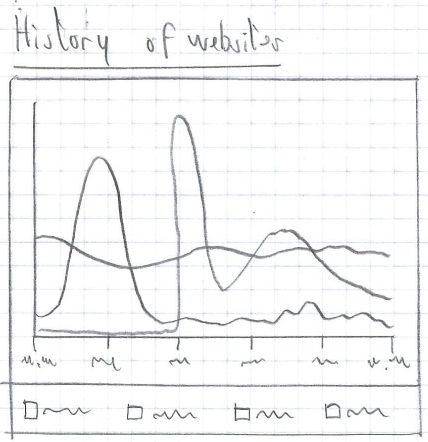
\includegraphics[width=0.3\textwidth,valign=t]{images/design/pages/history_mockup}}
			\subfloat[Exemple de résultat final]{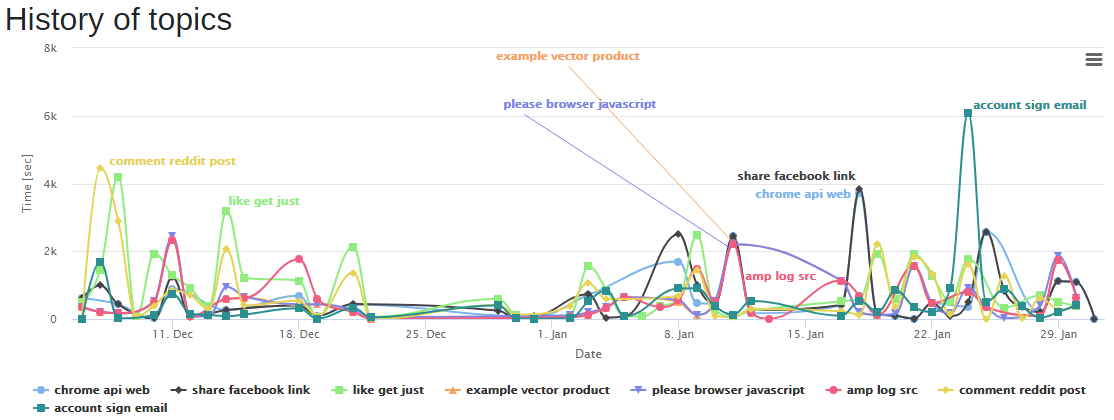
\includegraphics[width=0.7\textwidth,valign=t]{images/design/pages/history_final}}
			\caption{Maquette initiale et résultat final de la vue History}
			\label{history_images}
		\end{figure}

	\subsection{Données}

		Les données source servant à constituer cette visualisation sont :
		\begin{description}
			\item[Temps de visualisation] : Temps de visualisation total de chaque page. Ces données sont stockées dans la table \texttt{pagewatch} (figure \ref{table-content}).
			\item[Historique de visualisation] : Temps passé par jour sur chaque URL. Les données non agrégées proviennent de la table \texttt{pageviews} (figure \ref{table-pagewatch}).
			\item[Poids TF-IDF] : Poids final selon l'algorithme TF-IDF de chaque mot. Ces données sont stockées dans la table \texttt{computed\_tfidf} (figure \ref{table-computed-tfidf}).
			\item[Topics LDA] : Liste des topics générés par le modèle LDA. Ces données sont stockées dans la table \texttt{lda\_topics} (figure \ref{table-lda-topics}).
		\end{description}

	\subsection{Traitement}

		Afin de déterminer quels sont les topics et les mots cumulant le plus d'intérêt, il est nécessaire de disposer de plusieurs sources de données et de les assembler afin d'arriver au résultat voulu. Ceci se fait en plusieurs étapes, distribuées entre le serveur et client.

		L'algorithme suivant, illustré par la figure~\ref{history_algo}, est appliqué aux données sources :
		\begin{description}
			\item[A] On calcule le poids de chaque mot dans chaque document en effectuant la méthode de TF-IDF.

			\item[B] On entraîne un modèle LDA avec un nombre défini de topics (typiquement 100) sur le contenu de l'ensemble des pages web, une page web représentant un document.
			
			Une fois le modèle LDA entraîné, on lui demande la liste des 100 topics générés par leur représentation en 5 mots. Cette liste de topics est enregistrée dans la base de données.

			\item[C] Pour chaque page enregistrée, on demande au modèle LDA quels sont les 5 topics les plus probables avec leur score de probabilité. Ces informations sont également enregistrées dans la base de données. Jusqu'ici, toutes ces opérations sont donc déjà calculées et se font avant le lancement du serveur. Elles ne sont pas mises à jour en temps réel.

			\item[D] On demande à la base de données de grouper le temps de visionnage (en secondes) en une somme par jour et par URL différente. Ceci se fait au travers d'une commande MySQL et est calculé en temps réel, et s'occupe également d'"arrondir" chaque date de visualisation d'une page à la journée (au lieu de la seconde près, qui est la granularité utilisée dans la base de données).

			\item[E] Le résultat de l'étape précédente est disponible via l'endpoint\\
			\texttt{/api/historySites}.

			\item[F] On effectue la somme du temps que l'utilisateur a passé à regarder chaque page visitée. L'interface obtient ce résultat en appelant l'endpoint\\
			\texttt{/api/mostWatchedSites} du serveur. Le résultat de cet appel est une liste de l'ensemble des pages web regardées, comprenant entre autres une liste des mots les plus significatifs selon TF-IDF ainsi que leur poids TF-IDF (normalisé entre 0 et 1) pour chaque page.
			
			\item[G] L'endpoint \texttt{/api/allTopics} renvoie la liste des topics générés par LDA ainsi que leur numéro d'identifiant.

			\item[H] On cherche à savoir quels sont les mots où lesquels l'utilisateur a montré le plus d'intérêt afin de les afficher sur le graphe. Pour ceci, on multiplie la valeur TF-IDF de chaque mot par le temps passé à visualiser la page. La somme de ce calcul sur toutes les pages va nous donner l'"intérêt" final de l'utilisateur pour un mot particulier. On ne gardera ici que les 8 mots avec le plus grand intérêt estimé.

			\item[I] Finalement, pour chacun des 8 mots retenus, on affiche leur intérêt journalier sur le deuxième graphique, "Words history".

			\item[J] On cherche à savoir quels sont les topics où lesquels l'utilisateur a montré le plus d'intérêt afin de les afficher sur le graphe.

			Voici ce que l'on effectue sur chaque page : Pour chaque topic où sa valeur selon le modèle LDA sur cette page est au-dessus de 0.1, on estie que la page parle de ce topic et on compte le temps passé à visualiser la page dans la valeur de ce topic pour la journée.

			Finalement, on somme le temps passé sur chaque "topic". Le résultat de ce calcul sur toutes les pages va nous donner l'"intérêt" final de l'utilisateur pour un topic particulier. On ne gardera ici que les 8 topics avec le plus grand intérêt estimé.

			\item[K] Finalement, pour chacun des 8 topics retenus, on affiche leur intérêt journalier (qui est la même somme que précédamment, mais agrégée par jour au lieu de toute la période) sur le premier graphique, "Topics history".
		\end{description}

		\begin{figure}[!h]
			\centering
			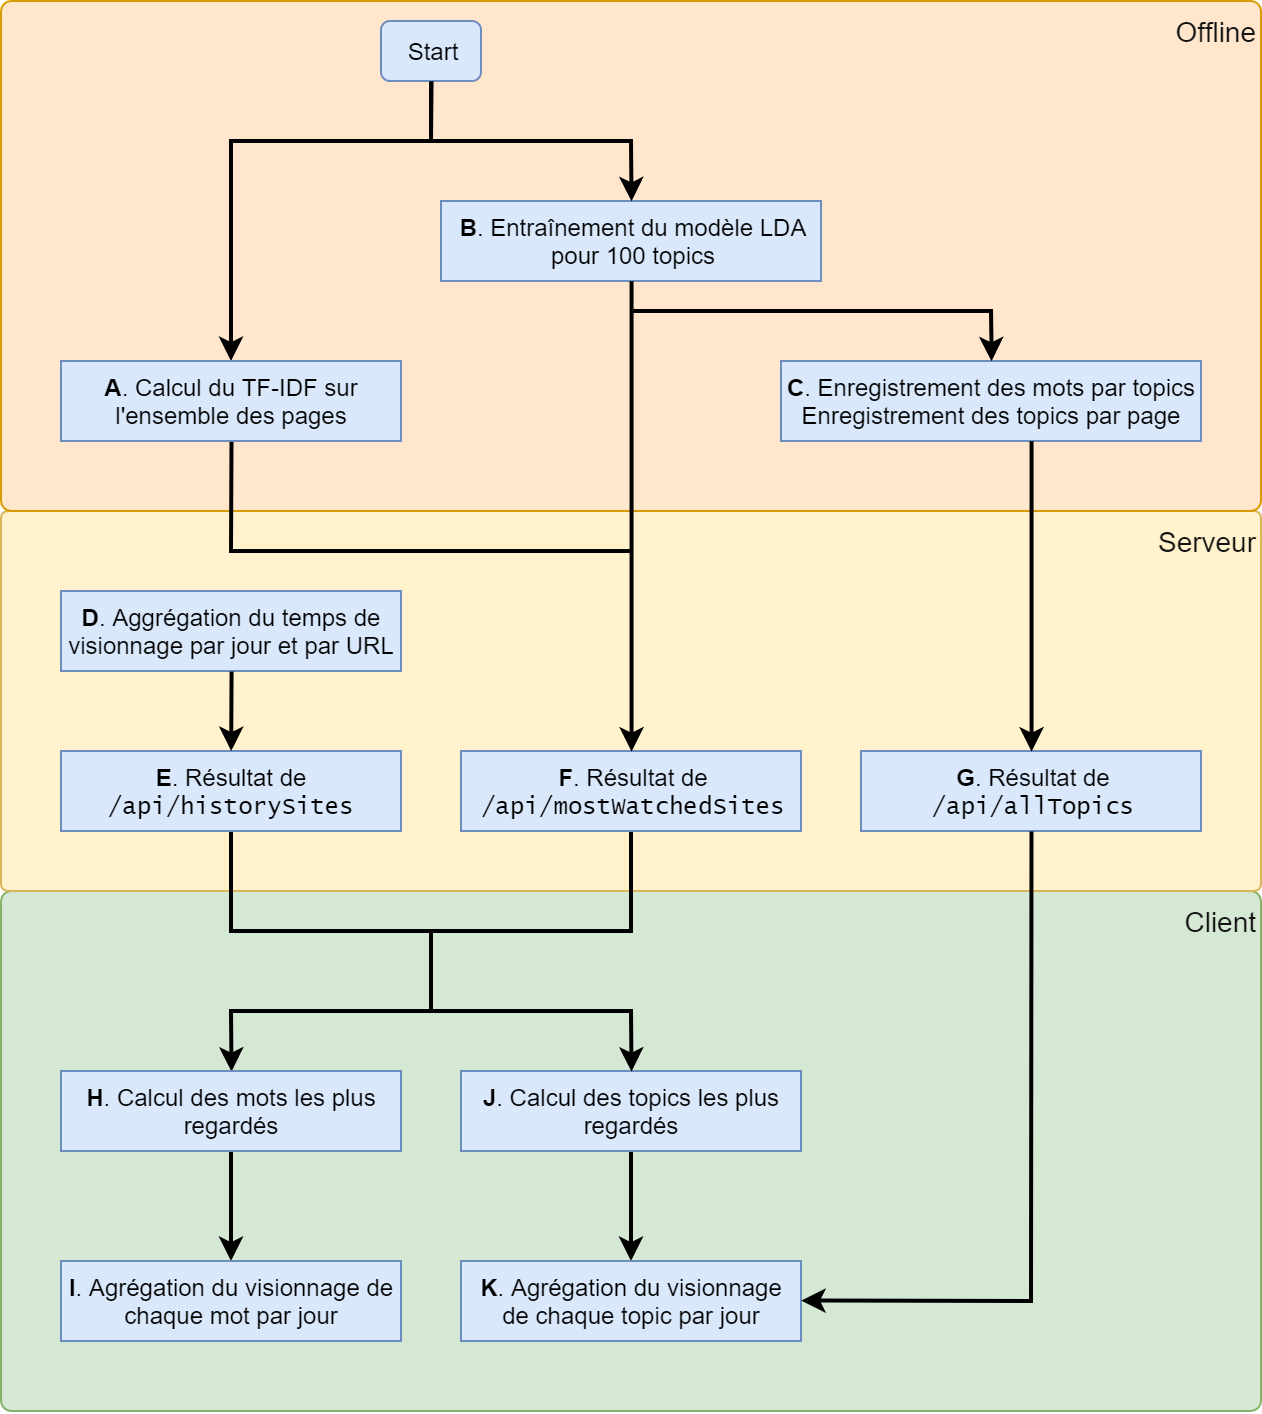
\includegraphics[height=1.15\textwidth]{images/design/pages/history_algo}
			\caption{Algorithme utilisé pour les graphiques de la page "History"}
			\label{history_algo}
		\end{figure}

	\subsection{Visualisation}

		Les données sont finalement transformées dans un format compatible et passées à une instance configurée de la librairie HighCharts, qui génère la visualisation du graphique sur la page.

\clearpage

%
%
% TRACKERS
%
%

\section{Trackers}

	\subsection{Concept}

		La vue "Trackers" comporte deux pages liées à une seule source de données. Le but est de montrer à l'utilisateur que lorsqu'une page web est visitée, des informations peuvent tout de même être transmises à d'autres domaines.

		La première vue de l'interface, "Most Sending", montre quels sont les domaines qui contactent beacoup des domaines différents. Il peut ainsi voir sur cette vue quels sont les serveurs qui sont contactés lorsqu'il accède à une page web.

		L'inverse est possible également. Grâce à la deuxième vue "Most recieving" il est possible de découvrir quels sont les domaines - trackers potentiels - qui sont fréquemment contactés par d'autres pages web. Chaque vue donne donc un point de vue différent sur le flux des données lorsque l'utilisateur parcourt le web.

		\begin{wrapfigure}{r}{3cm}
			
\includegraphics[width=2cm]{images/design/pages/trackers_button}
			\caption{Domaine activé, puis désactivé}\label{d-buttons}
		\end{wrapfigure} 

		De plus, ces deux vues peuvent interagir : Il est possible de décider de cacher certains domaines de l'une ou de l'autre vue, car par exemple l'utilisateur souhaiterait ne pas prendre en compte les données d'un certain site web, ou à l'inverse ignorer les données envoyées vers un potentiel tracker particulier.\\
		Un bouton permettant d'activer ou de désactiver les données du domaine est présent à chaque ligne, et la désactivation de celui-ci impacte la vue des données de l'ensemble des deux pages "Trackers". La figure~\ref{d-buttons} montre un bouton de domaine activé et désactivé.
		
		Ainsi il est par exemple possible de désactiver les données émises par un domaine, et de regarder quelle est la répercussion sur les données reçues par les autres.

		La figure~\ref{trackers_images} montre la différence entre la vue imaginée et le résultat final d'une des deux pages Trackers. La figure~\ref{tracker_images} montre la différence entre la vue imaginée et le résultat final de la page détaillée d'un tracker.

		\begin{figure}[p]
			\centering
			\subfloat[Maquette initiale de la vue]{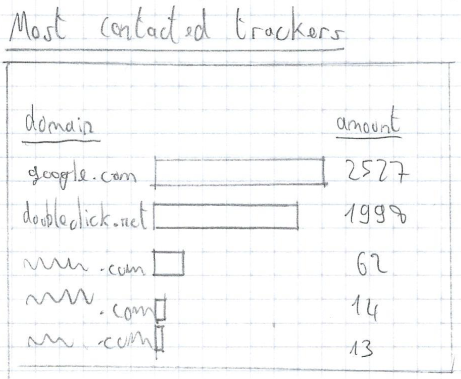
\includegraphics[width=0.3\textwidth,valign=t]{images/design/pages/trackers_mockup}}
			\subfloat[Exemple de résultat final]{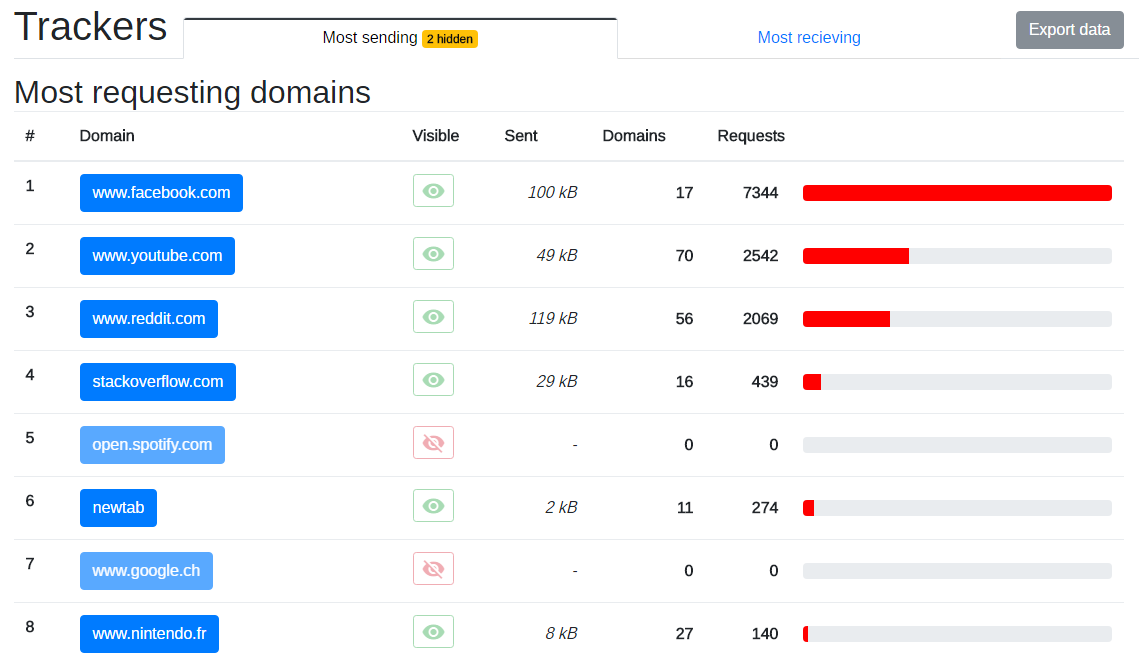
\includegraphics[width=0.75\textwidth,valign=t]{images/design/pages/trackers_final}}
			\caption{Maquette initiale et résultat final d'une des vues Trackers}
			\label{trackers_images}
		\end{figure}

		\begin{figure}[p]
			\centering
			\subfloat[Maquette initiale de la vue]{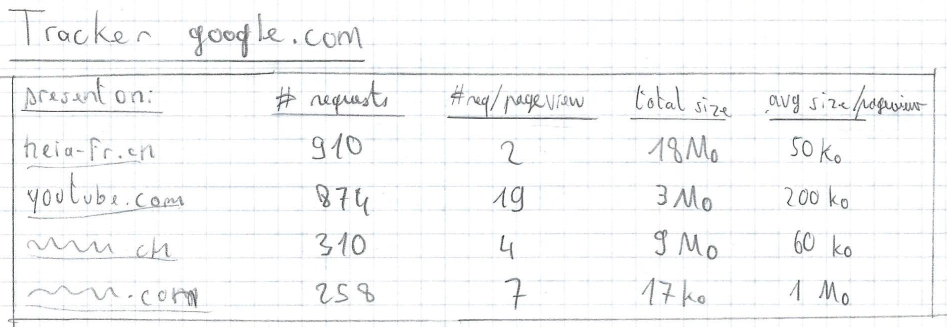
\includegraphics[width=0.6\textwidth,valign=t]{images/design/pages/tracker_mockup}}

			\subfloat[Exemple de résultat final]{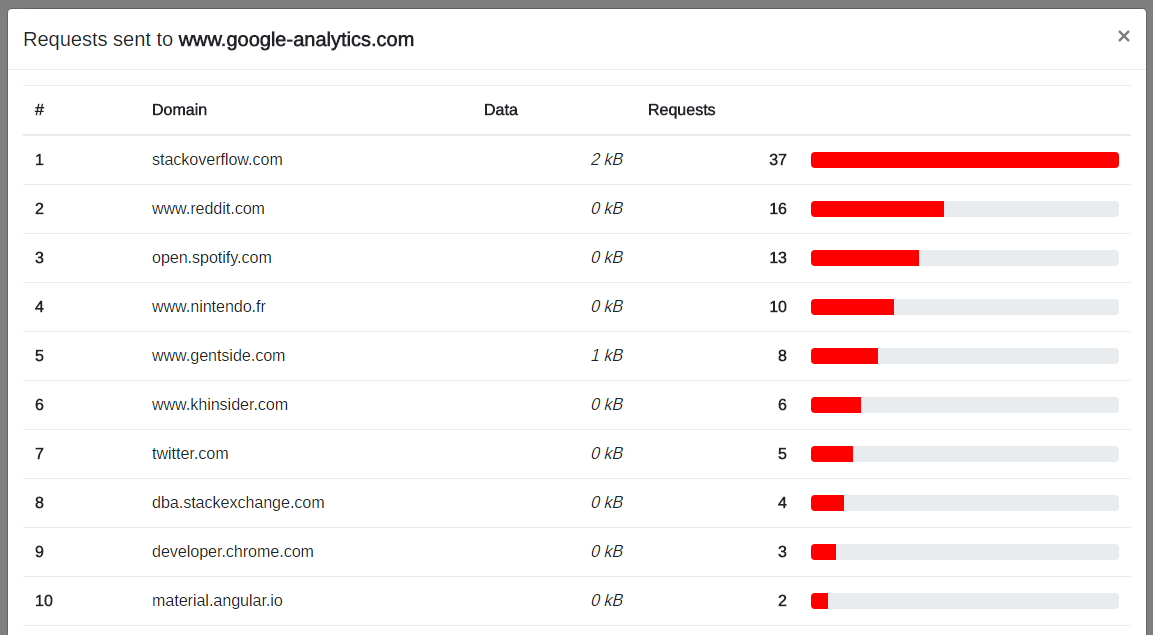
\includegraphics[width=0.75\textwidth,valign=t]{images/design/pages/tracker_final}}
			\caption{Maquette initiale et résultat final de la vue détaillée lors d'un clic sur un Tracker}
			\label{tracker_images}
		\end{figure}

		De plus, il est possible sur chacune des deux pages d'accéder aux statistiques détaillées sur le trafic de données d'un domaine particulier. En cliquant sur un domaine, l'interface ouvre une troisième vue qui montre en détail le nombre de requêtes liées à un domaine particulier.

	\newpage

	\subsection{Données}

		Une seule source de données est nécessaire à constituer cette visualisation :
		\begin{description}
			\item[Requêtes pré-calculées] : Nombre de requêtes entre chahque domaine. Ces données sont stockées dans la table \texttt{precalc\_trackers} (figure \ref{table-precalc-trackers}).
		\end{description}

		\FloatBarrier

	\subsection{Traitement}

		Peu de traitements entrent en jue dans la génération de la page Trackers. Il s'agit principalement de calculer la somme d'une liste de domaines. Ceci est illustré par la figure~\ref{trackers_algo} :
		\begin{description}
			\item[A] On additionne le nombre de requêtes faite pour un domaine vers un autre domaine, et on enregistre le total pour chaque paire par utilisateur. Toutes ces données sont pré-calculées avant le lancement du serveur. Il s'agit de calculer le nombre de requêtes de chaque domaine vers chaque autre domaine pour chaque utilisateur. La nécessité de pré-calculer ces données vient de leur quantité brute. Les compter sur le moment pour chaque requête demande trop de temps.

			\item[B] L'endpoint \texttt{/api/getTrackers} sert l'ensemble des résultats enregistrés pour l'utilisateur.

			\item[C] On cherche ici les domaines ayant reçu le plus de requêtes. Nous allons donc effectuer regrouper les requêtes faites par leur nom de domaine de destination, et effectuer la somme des autres mesures.

			\item[D] Inversément à l'étape précédente, on cherche cette fois les domaines ayant envoyé le plus de requêtes. Nous allons regrouper les requêtes par leur domaine d'envoie, et effectuer la somme des autres mesures.

			\item[E] Les deux listes obtenues aux étapes précédentes sont alors affichées dans leur page correspondante.

			\item[F] L'utilisateur peut choisir de cacher ou d'afficher un certain domaine d'une des vues. Ceci lance alors un nouveau calcul à partir de l'étape C. Aucune communication avec le serveur n'est nécessaire : Les données reçues initialement sont préservées.

			\item[G] L'utilisateur peut également choisir d'afficher les requêtes d'un domaine particulier.

			\item[H] Dans le cas de la sélection d'un domaine à afficher en détail, la liste des requêtes est filtrée est l'interface n'affiche que les requêtes concernant le domaine souhaité.
		\end{description}

		\begin{figure}[!h]
			\centering
			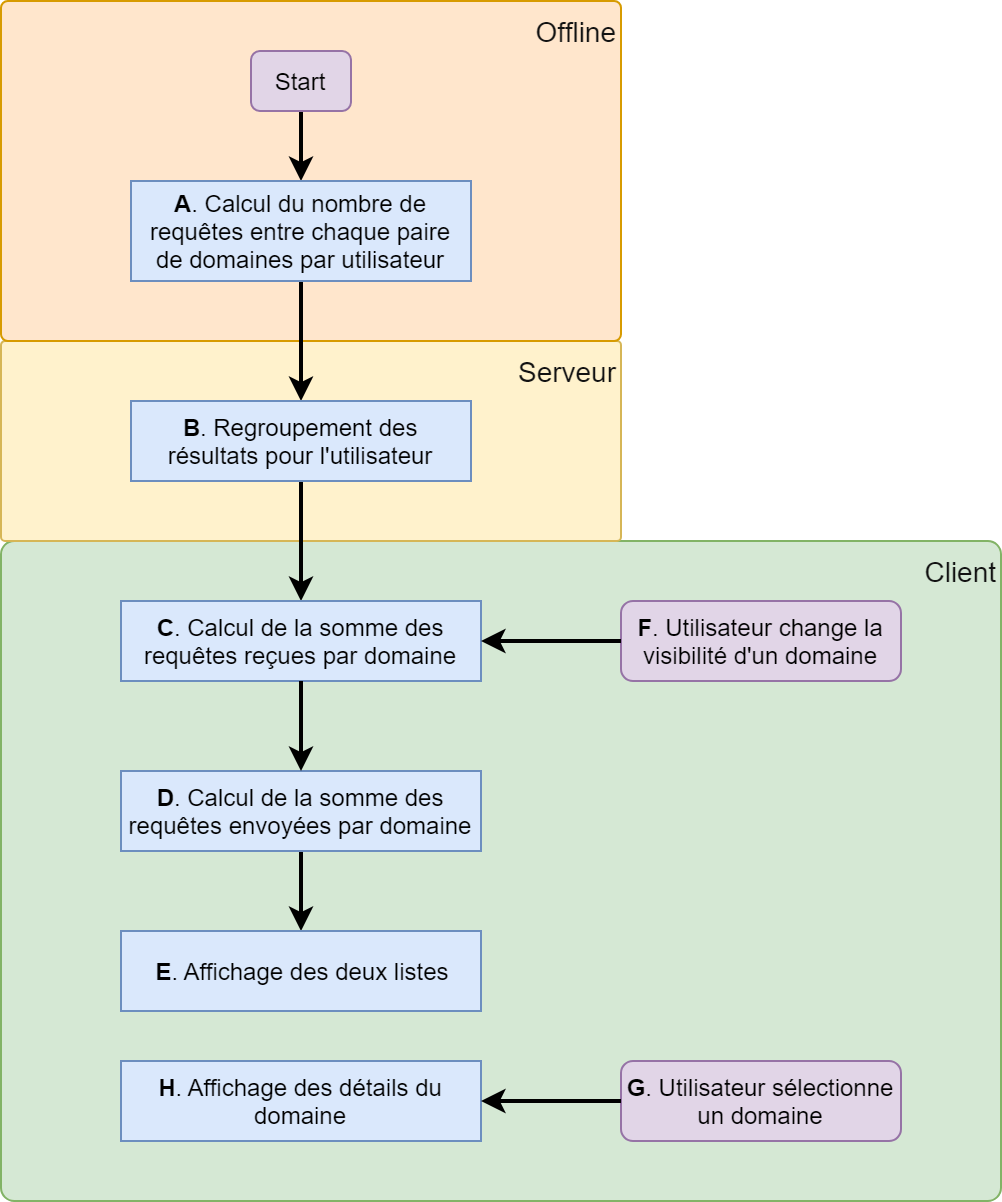
\includegraphics[height=0.95\textwidth]{images/design/pages/trackers_algo}
			\caption{Algorithme utilisé pour les données des pages "Trackers"}
			\label{trackers_algo}
		\end{figure}

	\subsection{Visualisation}

		Les deux listes sont des tableaux HTML stylisés par Bootstrap. La gestion de leur interaction et de leur affichage est géré par plusieurs composants Vue imbriqués.

\clearpage

%
%
% STATS
%
%

\section{Stats}

	\subsection{Concept}

		Le but de la vue Stats est de résumer très rapidement en quelques nombres la quantité de données échangées entre les différents domaines visités par l'utilisateur.

		\begin{figure}[!h]
			\centering
			\subfloat[Maquette initiale de la vue]{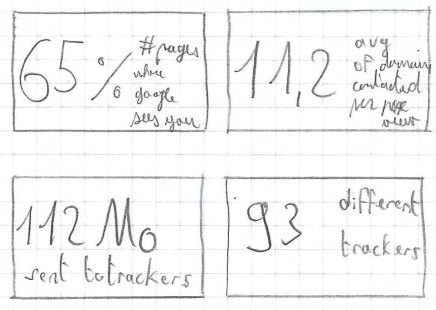
\includegraphics[width=0.3\textwidth,valign=t]{images/design/pages/stats_mockup}}
			\subfloat[Exemple de résultat final]{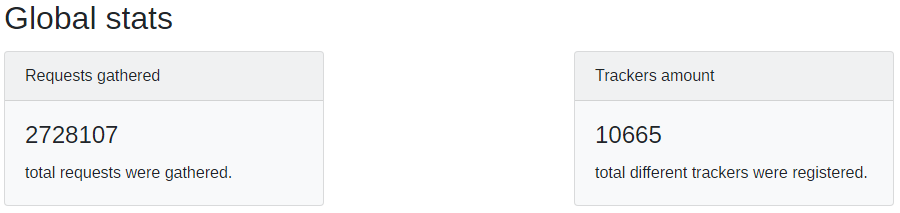
\includegraphics[width=0.7\textwidth,valign=t]{images/design/pages/stats_final}}
			\caption{Maquette initiale et résultat final d'une vue Stats}
			\label{stats_images}
		\end{figure}

	\subsection{Données}

		Une seule source de données est nécessaire à constituer cette visualisation :
		\begin{description}
			\item[Requêtes pré-calculées] : Nombre de requêtes entre chahque domaine. Ces données sont stockées dans la table \texttt{precalc\_trackers} (figure \ref{table-precalc-trackers}).
		\end{description}

	\subsection{Traitement}

		Très peu de traitements sont nécessaires pour cette vue. La figure~\ref{stats_algo} montre le traitement effectué aux données avant de les afficher.

		Les données nécessaires à cette vue sont calculées en temps réel : Il s'agit simplement de compter le nombre de requêtes enregistrées dans la table pré-calculée, ainsi que le nombre unique de nom de domaines.

		\begin{description}
			\item[A] On additionne le nombre de requêtes faite pour un domaine vers un autre domaine, et on enregistre le total pour chaque paire par utilisateur. Toutes ces données sont pré-calculées avant le lancement du serveur. Il s'agit de calculer le nombre de requêtes de chaque domaine vers chaque autre domaine pour chaque utilisateur. La nécessité de pré-calculer ces données vient de leur quantité brute. Les compter sur le moment pour chaque requête demande trop de temps.

			\item[B] On calcule le total de certaines valeurs pour les requêtes de l'utilisateur : Par exemple, le nombre total effectuées, et le nombre total de domaines différents.

			\item[C] On calcule ici certaines valeurs globales pour l'ensemble des utilisateurs. Par exemple le nombre total effectuées, et le nombre total de domaines différents.

			\item[D et E] On affiche les nombres résultats des opérations précédente dans leur page respective, à savoir "Your stats" présentant les statistiques de l'utilisateur uniquement, ou "Global stats" affichant les statistiques globales sur la base de données.

		\end{description}

		\begin{figure}[!h]
			\centering
			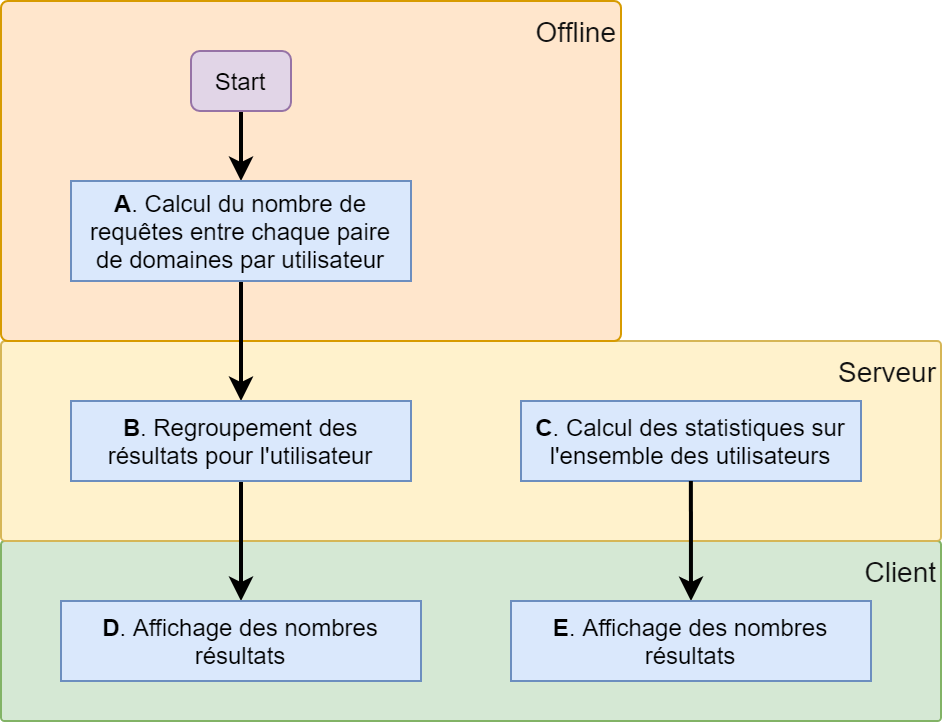
\includegraphics[height=0.6\textwidth]{images/design/pages/stats_algo}
			\caption{Algorithme utilisé sur les données de la page "Stats"}
			\label{stats_algo}
		\end{figure}

	\subsection{Visualisation}

		Les nombres renvoyées par le serveur sont simplement affichés dans des \texttt{card}s de Bootstrap.

\clearpage

%
%
% SETTINGS
%
%

\section{Settings}

	\subsection{Concept}

		Le but de la page Settings est de montrer à l'utilisateur la possibilité de renseigner ces centres d'intérêt. Ces informations nous seront utiles par la suite pour tenter d'associer les centres d'intérêt entrés ici avec les topics que nous estimons être importants.

		La figure~\ref{settings_image} montre un formulaire à remplir par l'utilisateur. Celui-ci cherche ces centres d'intérêts parmi une liste de 101, organisés hiérarchiquement. Un maximum de 10 centres d'intérêts peuvent être choisis.

		\begin{figure}[!h]
			\centering
			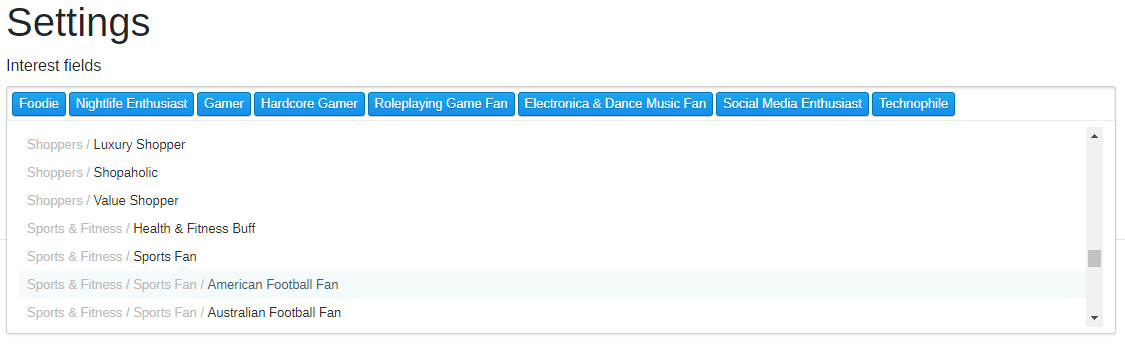
\includegraphics[height=0.32\textwidth]{images/design/pages/settings}
			\caption{Champ d'entrée des centres d'intérêts}
			\label{settings_image}
		\end{figure}

		Une fois que l'utilisateur a défini des centres d'intérêt, il peut donner des informations sur la page Topics (voir section \ref{topicslist}). Les centres d'intérêts choisis sur la page Settings sont donc "simplement" utilisés pour définir quels seront les choix de centres d'intérets possibles sur la page Topics List. La figure~\ref{choice} montre la fenêtre déroulante de sélection d'un centre d'intérêt pour un topic donné.

		\begin{figure}[!h]
			\centering
			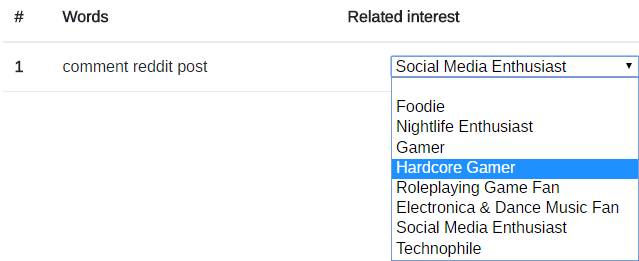
\includegraphics[height=0.32\textwidth]{images/results/choice}
			\caption{Sélection d'intérêt sur un topic}
			\label{choice}
		\end{figure}

		Il est demandé aux utilisateurs d'ajouter une association entre un topic et un intérêt lorsque cela semble lui faire sens. Ainsi, nous pouvons savoir quels topics de l'utilisateur nous avons réussi à identifier. En effet, lorsqu'un utilisateur associe un centre d'intérêt à un topic, celà signifie non seulement que le topic trouvé a du sens en soi, mais en plus qu'il est intéressant pour l'utilisateur.

	\subsection{Données}

		Deux source de données est nécessaire à constituer la vue Settings :
		\begin{description}
			\item[Liste des 101 centres d'intérêts] : Ces données sont stockées dans la table \texttt{interests} (figure \ref{table-interests}).
			\item[Centres d'intérêt de l'utilisateur] : Ces données sont stockées dans la table \texttt{user\_interests} (figure \ref{table-user-interests}).
		\end{description}

	\subsection{Traitement}

		Très peu de traitements sont nécessaires pour cette vue. La plupart des données nécessaires à cette vue sont calculées en temps réel : Il s'agit simplement de compter le nombre de requêtes enregistrées dans la table pré-calculée, ainsi que le nombre unique de nom de domaines.

		La figure~\ref{stats_algo} montre le traitement effectué aux données avant de les afficher.

		\begin{description}
			\item[A] La liste pré-définie de centres d'intérêts est ajoutée à la base de données. Cette opération n'est à effectuer qu'une seule fois, le but de cette liste n'est pas de changer. Dans notre cas, la liste des centres d'intérêts provient de ceux utilisés par la classification des utilisateurs par Google.

			\item[B] On envoie la liste des centres d'intérêts et de leur nom au client

			\item[C] On envoie également la liste des centres d'intérets que l'utilisateur a déjà renseignés, afin de les afficher directement comme étant entrés dans le formulaire.

			\item[E] L'utilisateur peut donc changer ses centres d'intérêts, puis envoyer sa nouvelle liste au serveur.

			\item[F] Les nouveaux centres d'intérêts sont donc enregistrés, et la nouvelle liste est envoyée une fois supplémentaire cu lient, reprenant au point C de l'algorithme.

		\end{description}

		\begin{figure}[!h]
			\centering
			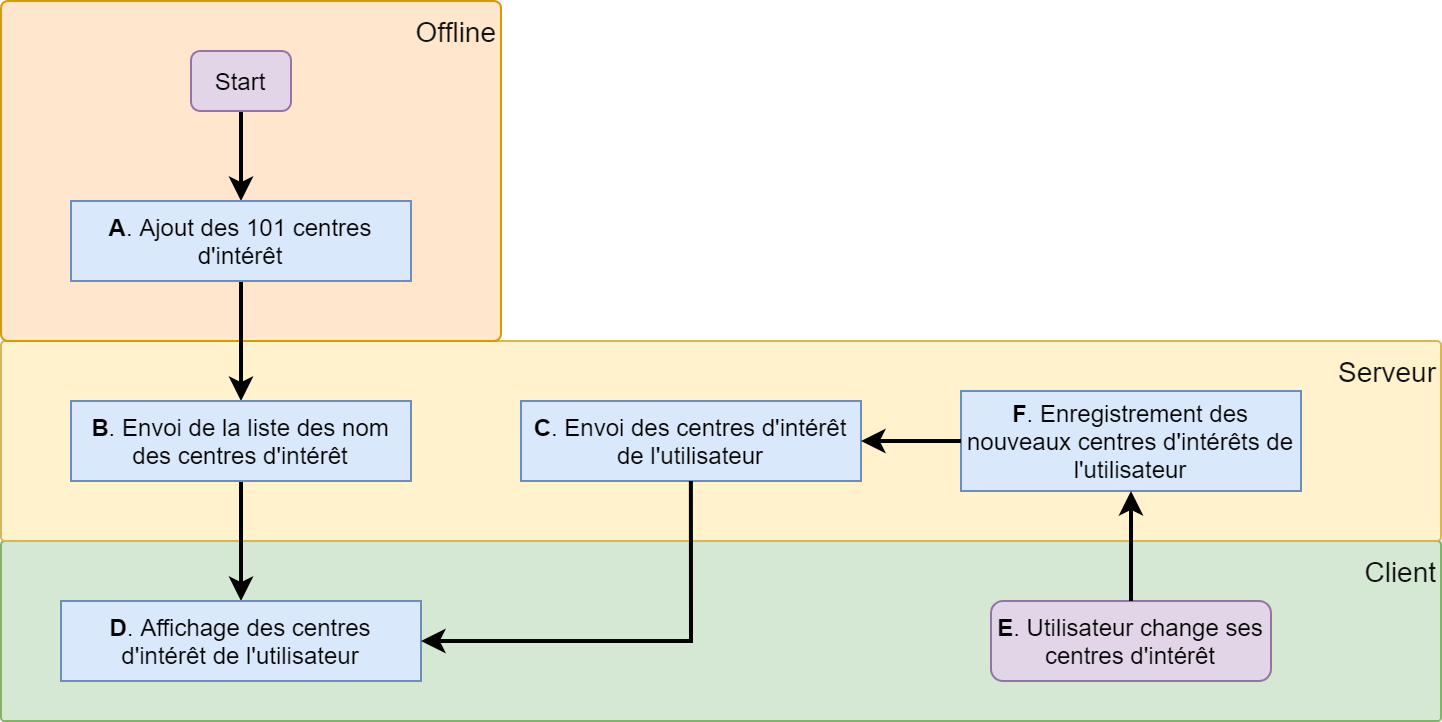
\includegraphics[height=0.52\textwidth]{images/design/pages/settings_algo}
			\caption{Algorithme utilisé pour les données de la page "Settings"}
			\label{settings_algo}
		\end{figure}

	\subsection{Visualisation}

		Le champ du formulaire permettant d'entrer des centres d'intérêts en affichant leur hiérarchisation est une instance configurée de la librairie JavaScript nommée Selectize\cite{selectize}, dont le but est de proposer des champs de formulaire personnalisés tels que celui-ci.

\clearpage
\chapter{Résultats}
%%%%%%%%%%%%%%%%%%%%%%%%%%
%                          %
% ----- INTRODUCTION ----- %
%                          %
%%%%%%%%%%%%%%%%%%%%%%%%%%

\section{Test utilisateurs}

	Une fois toutes les parties du projet réalisées, à savoir l'extension navigateur, le serveur et l'interface, nous avons cherché des utilisateurs volontaires pour installer l'extension et l'utiliser pendant une période de 4 semaines. Bien qu'initialement prévue pour un grand panel d'utilisateurs, les restrictions temporelles ont limité la quantité d'utilisateurs que nous avons pu atteindre.

	Un total de 10 utilisateurs volontaires ont installé l'extension. Parmi eux, 8 ont été identifiés comme ayant une activité de navigation  sur Chrome assez grande pour contribuer à l'étude. (Ceux étant jugés inactifs totalisent moins de 10 minutes d'activité).

	\subsection{Inputs}

		En plus de récolter les données des utilisateurs et de les afficher, il leur a également été demandé de remplir quelques informations sur eux-même afin de pouvoir valider certains points de notre étude. Deux formulaires ont été mis en place à cette fin.

		\subsubsection{Centres d'intérêts}

			La figure~\ref{settings_image} montre un premier formulaire à remplir par l'utilisateur. Accessible via le lien vers la page "Settings", on lui demande ici de trouver et renseigner quelques uns de ces centres d'intérêt parmi une centaine.

			\begin{figure}[!h]
				\centering
				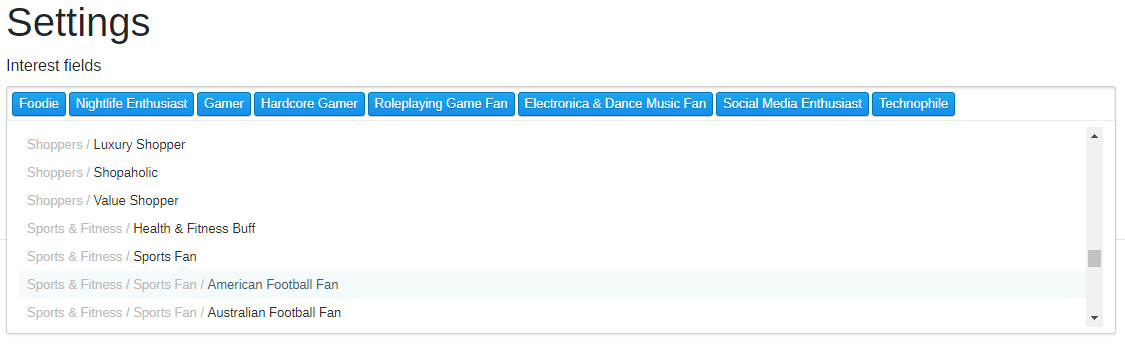
\includegraphics[height=0.32\textwidth]{images/design/pages/settings}
				\caption{Champ d'entrée des centres d'intérêts}
				\label{settings_image}
			\end{figure}

			Un maximum de 10 centres d'intérêts peuvent être définis. Le but de laisser à l'utilisateur entrer des centres d'intérêts est de pouvoir nous rendre compte si les topics que nous lui proposons sont proches de ces centres d'intérêt.

		\subsubsection{Association topic et intérêt}

			Une fois que l'utilisateur a défini des centres d'intérêt, il peut donner des informations sur les topics que nous lui suggérons sur la page Topics List (voir section \ref{topicslist}). La figure~\ref{choice} montre la fenêtre déroulante de sélection d'un centre d'intérêt pour un topic donné.

			\begin{figure}[!h]
				\centering
				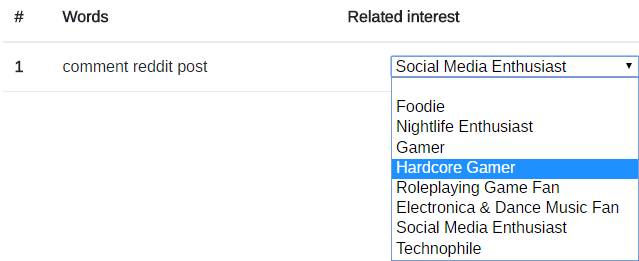
\includegraphics[height=0.32\textwidth]{images/results/choice}
				\caption{Sélection d'intérêt sur un topic}
				\label{choice}
			\end{figure}

			Il est demandé aux utilisateurs d'ajouter une association entre un topic et un intérêt lorsque cela semble lui faire sens. Ainsi, nous pouvons savoir quels topics de l'utilisateur nous avons réussi à identifier. En effet, lorsqu'un utilisateur associe un centre d'intérêt à un topic, celà signifie non seulement que le topic trouvé a du sens en soi, mais en plus qu'il est intéressant pour l'utilisateur.

			Sur l'échantillon de 8 personnes actives, 6 personnes ont ajouté des associations aux 20 topics proposés sur leur page. 

\section{Résultats de la recherche}

	Après une récolte des données sur environ 4 semaines, nous pouvons nous intéresser aux résultats que nous avons récoltés.

	\subsection{Modèles}

		Une première étape est de se pencher sur les modèles que nous avons généré sur la base des données elle-mêmes. Nous utilisons principalement deux algorithmes qui se basent sur le contenu des pages pour en déterminer leur thème : TF-IDF, et LDA.

		Ces modèles se basent sur le contenu des pages visitées des utilisateurs. Etant donné que nous ne récupérons pas directement le contenu de la page visitée par un utilisateur mais uniquement une partie de son URL, nous ne pouvons pas garantir que le contenu que nous récupérons d'une page soit effectivement le contenu que l'utilisateur voit sur son écran. En effet, beaucoup de pages web aujourd'hui sont liées à une application qui demande une authentification de l'utilisateur pour être affichée.

		Par exemple, une grande partie des pages d'un réseau social peuvent nécessiter la connexion de l'utilisateur pour être affichée.

		\subsubsection{TF-IDF}

			\paragraph{Résultats}

				Le fonctionnement de TF-IDF est décrit à la section \ref{analyse-tfidf}. Juger les résultats du calcul de TF-IDF sur des documents est une tâche non triviale. Cela revient principalement à vérifier manuellement que les mots ayant le poids le plus élevé pour certaines pages soit significatif de leur sujet.

				Intéressons-nous donc aux mots ayant le plus de poids trouvés pour les 20 pages les plus regardées, par exemple. Le tableau\ref{table-tfidf} illustre les 20 pages les plus regardées avec leurs mots associés, ainsi que plusieurs étapes amenant à une estimation finale de l'adéquation des mota trouvés avec le contenu de la page. Voici comment se lit le tableau :
				\begin{description}
					\item[URL] URL de la page concernée. Certaines URLs trop longues ont été raccourcies ici
					\item[Mot 1, 2, 3] 3 meilleurs mots dans l'orrdre décroissant décrivant la page selon TF-IDF.
					\item[Pub(lique)] Est-ce que la page nécessite une connexion afin d'accéder à son contenu principal.
					\item[Con(tenu)] Est-ce que le principal contenu de la page est textuel ?
					\item[Mot] Est-ce que chacun des mots trouvés sur la page fait sens dans une langue connue ?
					\item[Adé(quat)] Est-ce que l'ensemble des mots trouvés forme un potentiel résumé adéquat du contenu de la page ?
				\end{description}

				Les 4 premières colonnes (URL et 3 mots) proviennent de la base de données, tandis que les 4 dernières colonnes sont le résultat d'une évaluation manuelle des critères décrits. Un "OUI" dans une colonne indique que la page a passé le critère défini, contrairement à un "NON". Un "NON" dans une colonne entraîne automatiquement un "NON" dans les colonnes situées les plus à droite.

\begin{sidewaysfigure}
\centering
\caption{20 URLs les plus regardées et leurs meilleurs mots selon TF-IDF}
\label{table-tfidf}
\begin{tabular}{llllllll}
\textbf{URL}                                          & \textbf{Mot 1}  & \textbf{Mot 2}           & \textbf{Mot 3} & \textbf{Pub}           & \textbf{Con}            & \textbf{Mot}               & \textbf{Adé}            \\ \hline
\scriptsize \url{http://wdf.sdipi.ch/}                              & footprints      & digital                  & web            & \cellcolor[HTML]{9AFF99}OUI & \cellcolor[HTML]{9AFF99}OUI & \cellcolor[HTML]{9AFF99}OUI & \cellcolor[HTML]{9AFF99}OUI \\
\scriptsize \url{https://www.draw.io/}                                  & gmdl            & eng                      & proc           & \cellcolor[HTML]{9AFF99}OUI & \cellcolor[HTML]{FFCCC9}NON & \cellcolor[HTML]{FFCCC9}NON & \cellcolor[HTML]{FFCCC9}NON \\
\scriptsize \url{https://www.reddit.com/r/videos/}                      & submit          & load                     & report         & \cellcolor[HTML]{9AFF99}OUI & \cellcolor[HTML]{9AFF99}OUI & \cellcolor[HTML]{9AFF99}OUI & \cellcolor[HTML]{FFCCC9}NON \\
\scriptsize \url{https://www.google.co.uk/search}                       & eingabetaste    & suche                    & drücke         & \cellcolor[HTML]{9AFF99}OUI & \cellcolor[HTML]{FFCCC9}NON & \cellcolor[HTML]{FFCCC9}NON & \cellcolor[HTML]{FFCCC9}NON \\
\scriptsize \url{https://www.google.ch/search}                          & eingabetaste    & suche                    & drücke         & \cellcolor[HTML]{9AFF99}OUI & \cellcolor[HTML]{FFCCC9}NON & \cellcolor[HTML]{FFCCC9}NON & \cellcolor[HTML]{FFCCC9}NON \\
\scriptsize \url{http://game110.idlekiller.com/}                        & explorer        & chrome                   & browser        & \cellcolor[HTML]{9AFF99}OUI & \cellcolor[HTML]{9AFF99}OUI & \cellcolor[HTML]{9AFF99}OUI & \cellcolor[HTML]{9AFF99}OUI \\
\scriptsize \url{http://df.sdipi.ch/phpmyadmin/sql.php}                 & phpmyadmin      & past                     & welcome        & \cellcolor[HTML]{FFCCC9}NON & \cellcolor[HTML]{FFCCC9}NON & \cellcolor[HTML]{FFCCC9}NON & \cellcolor[HTML]{FFCCC9}NON \\
\scriptsize \url{https://web.whatsapp.com/}                             & whatsapp        & macos                    & mozilla        & \cellcolor[HTML]{FFCCC9}NON & \cellcolor[HTML]{FFCCC9}NON & \cellcolor[HTML]{FFCCC9}NON & \cellcolor[HTML]{FFCCC9}NON \\
\scriptsize \url{http://hexaclicker.github.io/}                         & hexa            & dp                       & level          & \cellcolor[HTML]{9AFF99}OUI & \cellcolor[HTML]{9AFF99}OUI & \cellcolor[HTML]{9AFF99}OUI & \cellcolor[HTML]{9AFF99}OUI \\
\scriptsize \url{http://blankmediagames.com/TownOfSalem/}              & salem           & adobe                    & town           & \cellcolor[HTML]{9AFF99}OUI & \cellcolor[HTML]{FFCCC9}NON & \cellcolor[HTML]{FFCCC9}NON & \cellcolor[HTML]{FFCCC9}NON \\
\scriptsize \url{http://www.jeuxvideo.com/}                             & jeu             & annonce                  & bande          & \cellcolor[HTML]{9AFF99}OUI & \cellcolor[HTML]{9AFF99}OUI & \cellcolor[HTML]{9AFF99}OUI & \cellcolor[HTML]{9AFF99}OUI \\
\scriptsize \url{https://discordapp.com/channels/217...408/217...408}   & own             & respective               & owner          & \cellcolor[HTML]{FFCCC9}NON & \cellcolor[HTML]{FFCCC9}NON & \cellcolor[HTML]{FFCCC9}NON & \cellcolor[HTML]{FFCCC9}NON \\
\scriptsize \url{https://www.reddit.com/r/leagueoflegends/}             & leagueoflegends & submit                   & self           & \cellcolor[HTML]{9AFF99}OUI & \cellcolor[HTML]{9AFF99}OUI & \cellcolor[HTML]{9AFF99}OUI & \cellcolor[HTML]{9AFF99}OUI \\
\scriptsize \url{https://www.reddit.com/}                               & bot             & agent                    & pardner        & \cellcolor[HTML]{9AFF99}OUI & \cellcolor[HTML]{9AFF99}OUI & \cellcolor[HTML]{9AFF99}OUI & \cellcolor[HTML]{FFCCC9}NON \\
\scriptsize \url{https://www.google.fr/search}                          & eingabetaste    & suche                    & drücke         & \cellcolor[HTML]{9AFF99}OUI & \cellcolor[HTML]{FFCCC9}NON & \cellcolor[HTML]{FFCCC9}NON & \cellcolor[HTML]{FFCCC9}NON \\
\scriptsize \url{https://s3-fr.gladiatus.gameforge.com/game/index.php}  & de              & gameforge                & vous           & \cellcolor[HTML]{FFCCC9}NON & \cellcolor[HTML]{FFCCC9}NON & \cellcolor[HTML]{FFCCC9}NON & \cellcolor[HTML]{FFCCC9}NON \\
\scriptsize \url{https://docs.google.com/presentation/d/1IB...l5w/edit} & row5w           & gecb...el5w & slide          & \cellcolor[HTML]{FFCCC9}NON & \cellcolor[HTML]{FFCCC9}NON & \cellcolor[HTML]{FFCCC9}NON & \cellcolor[HTML]{FFCCC9}NON \\
\scriptsize \url{https://twitter.com/}                                  & tweet           & foto                     & hast           & \cellcolor[HTML]{9AFF99}OUI & \cellcolor[HTML]{FFCCC9}NON & \cellcolor[HTML]{FFCCC9}NON & \cellcolor[HTML]{FFCCC9}NON \\
\scriptsize \url{http://df.sdipi.ch/phpmyadmin/db\_structure.php}       & phpmyadmin      & past                     & welcome        & \cellcolor[HTML]{FFCCC9}NON & \cellcolor[HTML]{FFCCC9}NON & \cellcolor[HTML]{FFCCC9}NON & \cellcolor[HTML]{FFCCC9}NON \\ \hline
\end{tabular}
\end{sidewaysfigure}

			\paragraph{Réflexion}

				Le fonctionnement de TF-IDF est décrit à la section \ref{analyse-lda}. Le tableau~\ref{resultats-tfidf} montre un résumé des résultats que l'on peut récupérer précédent tableau. On remarque que sur les 20 URLs entrées, seules 7 valent vraiment la peine d'être parcourues par notre algorithme, par élimination à causes des deux premières raisons énoncées. Cependant, sur les 7 URLs contenant du texte intéressant, TF-IDF a été capable d'en résumer adéquatement 5 d'entre-elles.

				Ce résultat est loin d'être parfait, mais il montre tout de même qu'il est possible d'automatiser la recherche de mots importants sur des pages lorsque les conditions sont favorables à notre approche.

\FloatBarrier

				\begin{table}[h]
\centering
\caption{Résumé des résultats de TF-IDF}
\label{resultats-tfidf}
\begin{tabular}{lr}
\textbf{URLs initiales}            & 20 \\
\textbf{Pages publiques}           & 14 \\
\textbf{Contenu textuel principal} & 7  \\
\textbf{Mots sensés}               & 7  \\
\textbf{Mots adéquats}             & 5 
\end{tabular}
\end{table}

		\subsubsection{LDA}

			\paragraph{Résultats}

				Dans la première semaine de récolte des résultats, une recherche empirique sur les paramètres à fournir au modèle a été effectuée. Le paramètre du nombre de topics a été fixé à 100; cela semblait un bon compromis, car 50 générait un nombre de trop restreint pour définir de manière assez précise quels étaient les thèmes d'un utisilateur, et 200 générait beaucoup de topics qui n'avaient pas de sens en eux-mêmes.

				La figure montre les 20 topics les plus 

			\paragraph{Réflexion}

	\subsection{Vues}

		\subsubsection{Wordcloud}

		\subsubsection{Topics List}

		\subsubsection{Most watched and viewed}

		\subsubsection{History}

		\subsubsection{Trackers}

	\subsection{Statistiques}

		\subsubsection{Profiling}

		\subsubsection{Trackers}

	\subsection{Implications}

\section{Conclusion}
\chapter{Conclusion}
%%%%%%%%%%%%%%%%%%%%%%%%%%%%%%
%                               %
% ----- CONCLUSION PROJET ----- %
%                               %
%%%%%%%%%%%%%%%%%%%%%%%%%%%%%%

\section{Conclusion du projet}

	\subsection{Délivrables}

		Ce projet est passé par plusieurs étapes distinctes qui ont mené à la production de plusieurs délivrables :
		\begin{itemize}
			\item Analyse des besoins
			\item Analyse des technologies
			\item Truc 1
			\item Truc 2
		\end{itemize}
		Chacune de ces étapes nous a amené à produire une itération supplémentaire contenant des nouveautés fonctionnelles.

	\subsection{Conclusion générale}

		Blabla
		\begin{itemize}
			\item Truc 1
			\item Truc 2
		\end{itemize}
		

	\subsection{Perspectives}

		Le projet dans son état final contient plusieurs pages non implémentées :

		\begin{itemize}
			\item Truc 1
			\item Truc 2
		\end{itemize}

%%%%%%%%%%%%%%%%%%%%%%%%%%%%%%%%%%%
%                                    %
% ----- CONCLUSION PERSONNELLE ----- %
%                                    %
%%%%%%%%%%%%%%%%%%%%%%%%%%%%%%%%%%%

\section{Conclusion personnelle}

	Blabla.

\begin{thebibliography}{9}

\bibitem{michal-kosinski}
  Michal Kosinski,
  \emph{Dr Michal Kosinski},
  \url{http://www.michalkosinski.com/},
  Consulté en ligne en Septembre 2017,
  2017.

\bibitem{mining-big-data}
  Michal Kosinski, Yilun Wang, Himabindu Lakkaraju and Jure Leskovec,
  \emph{Mining Big Data to Extract Patterns and Predict Real-Life Outcomes},
  \url{http://psycnet.apa.org/fulltext/2016-57141-003.pdf},
  Consulté en ligne en Octobre 2017,
  2017.

\bibitem{digital-footprints}
  Internet Society,
  \emph{Digital Footprints},
  \url{https://www.internetsociety.org/wp-content/uploads/2017/08/Digital20Footprints20-20An20Internet20Society20Reference20Framework.pdf},
  Consulté en ligne en Novembre 2017,
  Janvier 2014.

\bibitem{motherboard-data}
  Motherboard,
  \emph{The Data That Turned the World Upside Down},
  \url{https://motherboard.vice.com/en_us/article/mg9vvn/how-our-likes-helped-trump-win},
  Consulté en ligne en Octobre 2017,
  Janvier 2017.

\bibitem{kosinski-talk}
  Michal Kosinski,
  \emph{The End of Privacy, Keynote at CeBIT'17},
  \url{https://www.youtube.com/watch?v=DYhAM34Hhzc},
  Consulté en ligne en Octobre 2017,
  Mars 2017.

\bibitem{kaggle}
  Kaggle,
  \emph{Young People Survey},
  \url{https://www.kaggle.com/miroslavsabo/young-people-survey},
  Consulté en ligne en Octobre 2017,
  2013.

\bibitem{mypersonnality}
  Michal Kosinski,
  \emph{myPersonnality Project},
  \url{http://mypersonality.org},
  Consulté en ligne en Octobre 2017,
  2013.

\bibitem{analytics}
  Google,
  \emph{Google Solutions Analytics},
  \url{https://www.google.com/analytics},
  Consulté en ligne en Octobre 2017,
  2017.

\bibitem{analytics-usage}
  BuiltWith,
  \emph{Analytics Usage in Switzerland},
  \url{https://trends.builtwith.com/analytics/country/Switzerland},
  Consulté en ligne en Octobre 2017,
  2017.

\bibitem{chromewebstore}
  Chrome Web Store,
  \emph{Extensions},
  \url{https://chrome.google.com/webstore},
  Consulté en ligne en Novembre 2017,
  2017.

\bibitem{modulesfirefox}
  Modules Firefox,
  \emph{Extensions},
  \url{https://addons.mozilla.org/fr/firefox/extensions/},
  Consulté en ligne en Novembre 2017,
  2017.

\bibitem{timestats}
  Chrome Web Store,
  \emph{timeStats},
  \url{https://chrome.google.com/webstore/detail/timestats/ejifodhjoeeenihgfpjijjmpomaphmah},
  Consulté en ligne en Novembre 2017,
  2017.

\bibitem{ghostery}
  Ghostery,
  \emph{Ghostery makes the Web Cleaner, Faster and Safer!},
  \url{https://www.ghostery.com/},
  Consulté en ligne en Novembre 2017,
  2017.

\bibitem{privacymanager}
  Chrome Web Store,
  \emph{Privacy manager},
  \url{https://chrome.google.com/webstore/detail/privacy-manager/giccehglhacakcfemddmfhdkahamfcmd},
  Consulté en ligne en Novembre 2017,
  2017.

\bibitem{thegooddata}
  TheGoodData,
  \emph{TheGoodData},
  \url{https://thegooddata.org},
  Consulté en ligne en Novembre 2017,
  2017.

\bibitem{noiszy}
  Noiszy,
  \emph{Noiszy},
  \url{http://noiszy.com},
  Consulté en ligne en Novembre 2017,
  2017.

\bibitem{privacybadger}
  Modules pour Firefox,
  \emph{Privacy Badger},
  \url{https://addons.mozilla.org/fr/firefox/addon/privacy-badger17/},
  Consulté en ligne en Novembre 2017,
  2017.

\bibitem{krakenme}
  Kraken.me,
  \emph{Home},
  \url{http://www.kraken.me/#/home},
  Consulté en ligne en Novembre 2017,
  2017.

\bibitem{eff}
  Electronic Frontier Foundation,
  \emph{Defending your rights in the digital world},
  \url{https://www.eff.org},
  Consulté en ligne en Novembre 2017,
  2017.

\bibitem{nbdomains}
  HTTP Archive,
  \emph{Trends},
  \url{http://httparchive.org/trends.php?s=Top1000&minlabel=Oct+15+2011&maxlabel=Oct+16+2017#numDomains&maxDomainReqs},
  Consulté en ligne en Novembre 2017,
  2017.

\end{thebibliography}

\printglossary

\chapter*{Remerciements}
Je tiens à remercier ma superviseure Fatemi Nastaran pour m'avoir guidé lors des décisions à prendre, ainsi que Félicien Fleury pour m'avoir soutenu et guidé tout au long de ce projet.

\chapter*{Déclaration d'honneur}
Je, soussigné, Kewin Dousse, déclare sur l’honneur que le travail rendu est le fruit d’un travail personnel. Je certifie ne pas avoir eu recours au plagiat ou à toutes autres formes de fraudes. Toutes les sources d’information utilisées et les citations d’auteur ont été clairement mentionnées.

\bigskip
\bigskip

Lieu \hfil Date \hfil Signature

\appendix

\chapter{Historique des versions}
Voici l’historique des versions de ce document.

\begin{itemize}
	\item 0.1 : Template du document
	\item 0.2 : Chapitre "Analyse"
	\item 0.3 : Correction, complétion du chapitre "Analyse", rédaction d'une partie du chapitre "Conception"
	\item 0.4 : Rédaction de la plupart de la partie "Design du système", anciennement "Conception"
	\item 0.5 : Rédaction de la partie "Développement des vues"
	\item 0.6 : Complétion du "Développement des Vues", réorganisation de la structure de parties précédentes, et début de la partie "Résultats"
	\item 0.7 : Fin de la rédaction du texte du rapport
	\item 1.0 : Correction, complétion du chapitre "Analyse", ajout des annexes
\end{itemize}

\chapter{Cahier des charges}
\section{Activités}

Le développement du projet peut se découper en plusieurs phases, qui elles-mêmes se divisent en plusieurs activités. Voici la liste de ces activités :

\begin{enumerate}
	\item Analyse des besoins
	\begin{enumerate}
		\item Analyse des features demandées
		\item Etude des cas d’utilisation
		\item Etude de la faisabilité des demandes
		\item Analyse de la correspondance avec la base de données existante
	\end{enumerate}
	\item Analyse des technologies
	\begin{enumerate}
		\item Analyse et choix des technologies pertinentes
		\item Apprentissage des technologies choisies
	\end{enumerate}
	\item Conception de l’application
	\begin{enumerate}
		\item Design de l’architecture générale de l’application
		\item Design de l’interaction et de la structure de navigation
		\item Prototypage
	\end{enumerate}
	\item Réalisation de l’application
	\begin{enumerate}
		\item Réalisation du code backend
		\item Réalisation du code frontend
		\item Evaluation du comportement fonctionnel de l’application
		\item Evaluation de la robustesse de l’application
	\end{enumerate}
	\item Evaluation itérative
	\begin{enumerate}
		\item Evaluation formative
		\item Evaluation sommative informelle et empirique
		\item Rétrospective du développement
	\end{enumerate}
\end{enumerate}

\section{Planification}
Le projet comporte une série de dates-clé qu’il est important de respecter :
\begin{center}
   \begin{tabular}{ | l | c | r | }
     \hline
		Date & Semaine & Tâche \\ \hline
		\color{red}Lundi 20 février 2017 & Semaine P1 & Début du projet \\ \hline
		Lundi 31 mars 2017 & Semaine P6 & Fin de l’apprentissage des technologies choisies \\ \hline
		Lundi 20 mai 2017 & Semaine P12 & Fin de l’implémentation de l’application \\ \hline
		\color{red}Vendredi 9 juin 2017 & Semaine P15 & Dépôt du rapport \\ \hline
		\color{red}19-30 juin 2017 & - & Défense orale \\ \hline
     \hline
   \end{tabular}
\end{center}

Les dates en rouge sont des dates de rendu officielles.
Les autres représentent des jalons dans l’avancement du projet.

\section{Diagramme de Gantt}
	\includegraphics[width=0.51\textwidth]{images/annexes/cdc/gantt}

\chapter{Documentation}
\section{Localisation}

	L’ensemble des documents du projet est disponible à l’adresse suivante :
	\url{soon}

\section{Contenu}

	\subsection{GitLab}

	Le projet présent sur la forge contient toutes les versions de chacun des documents suivants, sous l’onglet « Documents » :
	\begin{itemize}
		\item Les procès-verbaux réalisés durant le projet.
	\end{itemize}


% \chapter{Code source}
% \section{README.md}
\lstinputlisting[title=README.md]{appendix/src/README.md}
\lstinputlisting[title=package.json]{appendix/src/package.json}
\lstinputlisting[title=webpack.config.json]{appendix/src/webpack.config.js}

% \lstinputlisting[title=README.md,language=md]{appendix/src/README.md}


\chapter{Procès-verbaux}
Voici les documents des procès-verbaux réalisés.

\newpage

\includegraphics[width=1\textwidth]{images/annexes/pvs/DigFootprints_PV_15_09_2017}

\includegraphics[width=1\textwidth]{images/annexes/pvs/DigFootprints_PV_21_09_2017}

\includegraphics[width=1\textwidth]{images/annexes/pvs/DigFootprints_PV_28_09_2017}

\includegraphics[width=1\textwidth]{images/annexes/pvs/DigFootprints_PV_05_10_2017}

\includegraphics[width=1\textwidth]{images/annexes/pvs/DigFootprints_PV_10_10_2017}

\includegraphics[width=1\textwidth]{images/annexes/pvs/DigFootprints_PV_12_10_2017}

\includegraphics[width=1\textwidth]{images/annexes/pvs/DigFootprints_PV_16_10_2017}

\includegraphics[width=1\textwidth]{images/annexes/pvs/DigFootprints_PV_26_10_2017}

\includegraphics[width=1\textwidth]{images/annexes/pvs/DigFootprints_PV_01_11_2017}

\includegraphics[width=1\textwidth]{images/annexes/pvs/DigFootprints_PV_09_11_2017}

\includegraphics[width=1\textwidth]{images/annexes/pvs/DigFootprints_PV_13_11_2017}

\includegraphics[width=1\textwidth]{images/annexes/pvs/DigFootprints_PV_16_11_2017}

\includegraphics[width=1\textwidth]{images/annexes/pvs/DigFootprints_PV_23_11_2017}

\includegraphics[width=1\textwidth]{images/annexes/pvs/DigFootprints_PV_30_11_2017}

\includegraphics[width=1\textwidth]{images/annexes/pvs/DigFootprints_PV_05_12_2017}

\includegraphics[width=1\textwidth]{images/annexes/pvs/DigFootprints_PV_07_12_2017}

\includegraphics[width=1\textwidth]{images/annexes/pvs/DigFootprints_PV_12_12_2017}

\includegraphics[width=1\textwidth]{images/annexes/pvs/DigFootprints_PV_21_12_2017}

\includegraphics[width=1\textwidth]{images/annexes/pvs/DigFootprints_PV_09_01_2018}

\includegraphics[width=1\textwidth]{images/annexes/pvs/DigFootprints_PV_18_01_2018}

\end{document}

% https://www.sharelatex.com/blog/2013/08/02/thesis-series-pt1.htmlx